\documentclass{ufpatcc}

\include{include}
%% Packages used for the TCC

%\usepackage{booktabs}

%%%% Definitions and New commnads %%%%

\newcommand{\sen}{\operatorname{sen}}
\newcommand{\mbeq}{\overset{!}{=}}

\renewcommand\Re{\operatorname{Re}}
\renewcommand\Im{\operatorname{Im}}

%%%% New control sequences %%%%

\newcommand{\redeq}[1] {\textcolor{red}{#1}}
\newcommand{\blueeq}[1] {\textcolor{blue}{#1}}
\newcommand{\att}[1] {\textcolor{red}{#1}}
% Used Packages:
\usepackage{tikz}
\usepackage{float}
\usepackage{steinmetz}
\usetikzlibrary{arrows,shapes,shapes.multipart}
%\usepackage[brazil]{babel}
\usepackage[T1]{fontenc}
\usepackage[utf8]{inputenc}
\usepackage{amsmath}
\usepackage{amsfonts}
\usepackage{enumitem} % To adjust lists
\usepackage{verbatim} % Multi-line comments
\usepackage{mathabx} % Package that contains the circular convolution symbol
\usepackage{graphicx}
\usepackage{caption}
\usepackage{subcaption}
\usepackage{units}
\usepackage{adjustbox}
\usepackage{dirtytalk}
\usepackage{csquotes}

%\usepackage[backend=bibtex8]{biblatex}

\ifpdf

\ifdefined\hyperref
\else
\usepackage[pdftex,colorlinks]{hyperref}
\fi

\hypersetup{%
pdftitle={Some title},
pdfauthor={Your name - LaPS - UFPA},
pdfkeywords={DSP,Signal},
pdfstartview={FitH}, %% <--
urlcolor=black,
%linkcolor=blue,
linkcolor=black,
%citecolor=red,
citecolor=black,
}

% Ensiar o Latex a separar silabas
\hyphenation{DMT En-ge-nhei-ro}


\ufpaTitulo{An FPGA-Based Radion Frontend for LTE Transmission on Cloud RAN}

\ufpaAutor{Gabriel Peixoto de Carvalho}
\ufpaSegundoAutor{}
\ufpaOrientador{Prof. Aldebaro Barreto da Rocha Klautau Junior}
\ufpaCoordenadorCurso{Prof. Jos\'{e} Augusto de Lima Barreiros}

\ufpaCoOrientador{Prof. Wilson Pacheco Ferreira}
\ufpaMembroBancaA{Prof. Francisco Carlos Bentes Frey Muller}
\ufpaMembroBancaB{Eng. Igor Mesquita de Almeida}


\begin{document}

\ufpaPaginaDeRosto

\ufpaPagRostodo

\ufpaPaginaDeAprovacao

%%%%%%%%%%%%%%%%%%%%
%   Oferecimento   %
%%%%%%%%%%%%%%%%%%%%

\begin{ufpaOferecimento}
\index{Oferecimento@Oferecimento}%
\addcontentsline{toc}{chapter}{Dedicat�ria}

\end{ufpaOferecimento}

%%%%%%%%%%%%%%%%%%%%
%  Agradecimento   %
%%%%%%%%%%%%%%%%%%%%

\begin{ufpaAgradecimentos}
\index{Agradecimentos@Agradecimentos}
\addcontentsline{toc}{chapter}{Agradecimentos}

\begin{flushright}
Gabriel Peixoto de Carvalho
\end{flushright}

\end{ufpaAgradecimentos}

%%%%%%%%%%%%%%%%%%%%
%      Ep�grafe     %
%%%%%%%%%%%%%%%%%%%%

\begin{ufpaEpigrafe}
Viva como se voc� fosse morrer amanh�. Aprenda como se voc� fosse viver para sempre.\\
\begin{flushright}Mahatma Gandhi\end{flushright}
\end{ufpaEpigrafe}

%%%%%%%%%%%%%%%%%%%%%
%  Lista de Siglas  %
%%%%%%%%%%%%%%%%%%%%%

\chapter*{Lista de Siglas} \label{sec:siglas}
\begin{enumerate}
 \item ADSL - \textit{Linha de assinante digital assim�trica}
 %\item AWGN - \textit{Ru�do aditivo branco Gaussiano}
 %\item BER - \textit{Taxa de erro de bit}
 %\item DFT - \textit{Transformada de Fourier discreta}
 %\item DMT - \textit{Multi-tom discreto}
 %\item DSL - \textit{Linha de assinante digital}
 %\item FEQ - \textit{Equalizador em frequ�ncia}
 %\item FFT - \textit{Transformada rápida de Fourier}
 %\item FTTH - \textit{Fibra até a residência}
 %\item G.fast - \textit{Acesso rápido aos terminais do assinante}
 %\item ICI - \textit{Interferência inter-portadora}
 %\item IDFT - \textit{Transformada de Fourier discreta inversa}
 %\item IFFT - \textit{Transformada rápida de Fourier inversa}
 %\item ISI - \textit{Interferência inter-simbólica}
 %\item OFDM - \textit{Modulação por divisão ortogonal de frequência}
 %\item PC - \textit{Prefixo cíclico}
 %\item PSD - \textit{Densidade espectral de potência}
 %\item RIC - \textit{Resposta impulsiva do canal}
 %\item SC - \textit{Sufixo cíclico}
 %\item SER - \textit{Taxa de erro de símbolo}
 %\item SNR - \textit{Razão sinal ruído}
 %\item VDSL - \textit{Linha de assinante digital com taxa de bit muito alta}
 %\item 4GBB - \textit{Quarta geração de banda larga}
\end{enumerate}
 


\chapter*{Lista de S�mbolos} \label{sec:simbolos}
\begin{description}[labelsep=5em, align=left,labelindent=2cm]
\item[$\Delta f$] Spacing between subcarriers
\item[$N$]        Number of Symbols
\item[$n$]        Index of Subcarrier
\item[$a$]        Amplitude
\item[$m$]        Index of OFDM symbol
\item[$sm$]       Useful OFDM symbol
\item[$T_u$]      Period of symbol Generation
\item[$T_s$]      Period of OFDM symbols
%\item[$n_0$] Indice da amostra de início do símbolo recebido para o receptor sincronizado
%\item[$N$] Número de pontos da DFT ou tamanho do vetor símbolo DMT
%\item[$N_a$] Número de amostras afetadas por ISI e ICI
%\item[$p_k$] Parte real do $k$-ésimo subsímbolo
%\item[$P_x$] Potência total de transmissão
%\item[$q_k$] Parte imaginária do $k$-ésimo subsímbolo
%\item[$\mathbf{Q}$] Matriz DFT
\end{description}


%%%%%%%%%%%%%%%%%%%%%%%%%%%%%%%%%%%%%%%%%%%%
%  Insere a lista de Figuras e de Tabelas  %
%%%%%%%%%%%%%%%%%%%%%%%%%%%%%%%%%%%%%%%%%%%%

\listoffigures \clearpage \listoftables \clearpage

%%%%%%%%%%%%%%%%%%%%
%      Sum�rio     %
%%%%%%%%%%%%%%%%%%%%

\tableofcontents    \clearpage

%%%%%%%%%%%%%%%%%%%%
%      Resumo      %
%%%%%%%%%%%%%%%%%%%%

\begin{ufpaResumo}


\end{ufpaResumo}

\begin{abstract}
    
The evolution of mobile services in terms of access technologies and application 
layers is driving a huge change in mobile communication systems. A recent hot 
topic in the field is the rise of the cloud computing paradigm, thus the idea 
known as cloud radio access networks (Cloud-RAN) is growing in the industry. 
This behavior comes from the potential of cloudification for improvement in the 
efficiency of resource allocation, manageability and power consumption, aspects 
inherent of traditional RANs.\\

Thus, with the emerging of C-RAN, several questions about how to implement and 
which tools to use come naturally. This work aims to evaluate the potential of a 
programmable fronthaul radio interface, as known, actual network does not have 
the adaptative capability needed for the C-RAN. For this work a setup of a radio 
unit, composed by two fpgas (one acting as the Baseband unit and other as the
(digital front-end) of the radio unity) connected through ethernet and two 
transceivers (analog front-end), one in each FPGA. Within this setup various 
algorithms can be tested and can be evaluated in LTE scenarios because the 
transceiver works in LTE and C-RAN .\\

This work shall focus on the evaluation of the radio interface and perform the 
tests inherent to it, exploring FPGA adaptability and parallelism with the 
internal and external communication protocols, and so exploring the advantages 
of the transceiver used, the fmcomms2  development board (AD9361 chip) from 
Analog devices, which is a device broadly used in software defined radio 
hardwares, as known as USRPs (Universal Software Radio Peripheral). \\

An aspect of the transceiver that is very attractive to the C-RAN paradigm is 
its configurability and scalability, capable of real-time adjustments in the 
sampling frequency or operation mode from 2x2 to 4x4 MIMO (Multiple Inputs and 
Multiple Outputs), this real-time adaptive characteristic is ideal to C-RAN 
environment.\\

The results are generated primarily aiming a fidelity in the transmitted and 
receiver signals, after these results are conclusive it is possible to proceed 
to more complex tests and approaches of this setup. Another test made was the 
analysis of the synchronization between  receiver and transceiver using a CIPRI 
emulator implemented in FPGA logic, which is the standard fronthaul interface, 
in this test it is possible to observe the advantages of the programmable radio 
front-end in the system.\\



\end{abstract}

%%%%%%%%%%%%%%%%%%%%%
%   Corpo do TCC    %
%%%%%%%%%%%%%%%%%%%%%

\pagenumbering{arabic}

\part{Introduction}
\chapter{Introduction}
\label{chap:intro}

The world is much more interconnected and the economy is growing wilder and
wilder, a lot of economical crisis rise in different countries almost every
year. The climate changes are also a concern to the modern governments, thus the
idea of re-utilizing resources and  make these resources be more economically
and environmentally friendly are a goal for modern research and development.\\

Cloud computing is a paradigm which is growing every year in the companies and
developers, it is not a magic method to solve all the problems but it solves
some infrastructure problems of small and big companies, where companies does
not need to won computers or anything locally to operate, everything can be done
remotely and a more experienced company and staff can offer such infrastructure
or application as a service. Such idea of having everything as a service is very
attractive both economically  and environmentally because there is no waste of
resource, everything is scalable to the need of the client and upgradeable if
needed.\\

The Radio access technologies have been evolving from audio traffic to
intensive data traffic over the recent standards, because the mobile devices
got a myriad of functions which could only be executed by Personal computers,
however the implementations of such networks demand a huge amount of resources
and with the economy becoming harder every year, there is the concern about how
to develop and deploy such networks and of course backwards compatibility of
these networks, because an operator would never deploy a network which is not
compatible with previous standards equipments, this is not profitable. Having
these ideas in mind the Centralized RAN idea began to be developed, such as
cloud computing, now there is the technology for the RANs to be scalable and
configurable to the needs of the clients and operators, where the baseband
processing is all done on the cloud and the radio front-ends are reconfigurable
to handle different data and modulation outputs.\\

The FPGA is very attractive to implement such radio front-ends and other
reconfigurable computing tasks, because it is flexible too be reconfigured
on-the-run and offers a really good processing and I/O capabilities. Thus this
work aims to evaluate the implementation feasibility of a radio front-end to
LTE transmissions (LTE band) in a Cloud RAN environment (adaptability and
reconfigurability).\\

This work is implemented in a Xilinx Virtex 7 FPGA and using the transceiver
FMComms2 from analog devices, this transceiver can be reconfigured in real time
and runs up to 6 GHz band, it has been chosen because of such reconfigurability
properties. This text is composed by 6 chapters divided in 5 parts.\\

The first part aims to introduce the environment in which this work was planned
with this introduction chapter. The second part is a literature review of
everything theoretical used in this work development, it is composed by two
chapters, the second chapter describing Cloud and Software defined radio
\ref{chap:sdr}, because this reconfigurability property has been widely
explored in software defined radio field. The third chapter is about Digital
communications and LTE, describing the basic blocks of digital communications
systems and briefly talking about LTE standard and how it is implemented
\ref{chap:lte}.\\

The third part is the core of the work, the implementation, in this chapter
the functionalities of both FPGA and transceiver shall be explained and the
work development will be described and how it was implemented in both FPGA
logic and software drivers \ref{chap:implementation}.\\

The fourth part reports all the results obtained in such work.The configuration
results report how the transceiver board communication and configuration were
succeed, the simulation results aim to show the VHDL blocks simulation prior to
hardware implementation and at last the transmission results \ref{chap:results}.

The last part is the conclusions and future works, which aim to report
everything learned from this work and what can be done to improve the
transmission/reception quality or communication \ref{chap:conclusion}.

\part{Literature Review}
\chapter{Carrier Recovery}

Carrier recovery is a processes used in coherent demodulation where the phase
and the frequency of the transmitter carrier wave are recovered by the receiver
and thus after having such information it is possible to extract the information
in the transmitted signal.\\
Considering that the phase and frequency of the transmitted wave probably will
be affected by noise, it is not a straight-forward method, it includes filtering
and usually feedback systems to correct the erros in phase or frequency caused
by the noise.\\
This chapter aims in the brief exploration of some techniques used for carrier
recovering, such as Phase locked loops, costas loop and others.\\

\section{Phase-Locked Loop (PLL)}
\label{sec:pll}

Phase-locked Loop is a kind of feedback system, which has been extensively used
in communications sytems and other applications which require frequency
synthesis.\\
The Phase-Locked Loop is composed by three basic components \ref{fig:pll}:

\begin{enumerate}
    \item A phase detector (PD).
    \item A loop filter.
    \item A voltage-controlled oscillator (VCO).
\end{enumerate}

As it can be seen in the figure \ref{fig:pll} the phase-locked loop is a feedback
system whose main goal is to make the output signal the same as the input
signal. Basically the phase detector compares the phase of the input signal
against the phase of the VCO output, then the PD output is inputed in the loop
filter whose output is the voltage that controls the VCO. The output of the
phase detector is the phase error between the input signal and the VCO and the
output of the loop filter outputs the control voltage to the VCO.\\

When the loop is locked, theoretically, the output frequency is the same as the
input frequency, but to maintain the control voltage necessary to lock it is
needed a nonzero output to the phase detector, thus the pll operates with some
phase error, but this tends to be small.\\

Pll makes simple to syntetize frequencies with a pll and do operations
of analog modulation and demodulation, these applications willbe briefly
discussed later.


\begin{figure}[htbp]
    \centering
    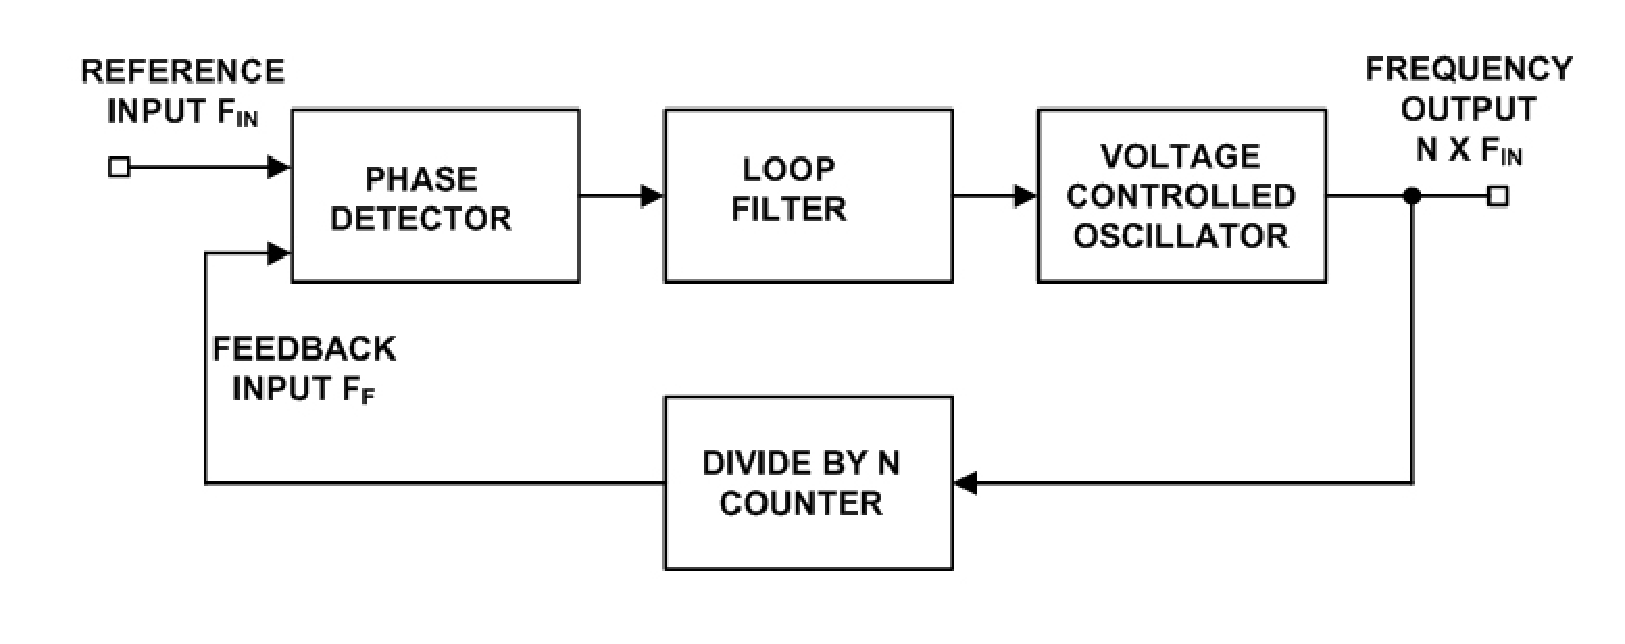
\includegraphics[width=0.65\textwidth]{./figures/pll.eps}
    \caption{ Basic PLL scheme
    \label{fig:pll}}
\end{figure}

\subsection{PLL Fundamentals}
Considering a basic pll scheme as shown in figure \ref{fig:pll2} we can see that
the input signal has a phase of $\theta_i(t)$ and the VCO output has a phase of
$\theta_o(t)$. Assuming that the loop is locked and the phase detector is
linear, the ouput of the PD is proportional to the phase difference between its
inputs, thus,

\begin{equation}
    v_d = K_d(\theta_i - theta_o)
    \label{eq:pdout}
\end{equation}

where $k_d$ is the PD gain factor and its unity is volt/radian.\\

The $v_d$ is filtered by the loop filter, supressing noise and high frequency
signal components, the filter also contributes for the determination of the
dynamic performance of the loop. The filter transfer function is given by
$F(s)$.

Frequency output of the VCO is determined by the input $v_c$ and since frequency
is the derivative of the phase, the operation in the VCO can be described by,

\begin{equation}
    L[\frac{d\theta_o(t)}{dt}] = s\theta_o(s)=K_oV_c(s)
    \label{eq:vco}
\end{equation}

\begin{figure}[htbp]
    \centering
    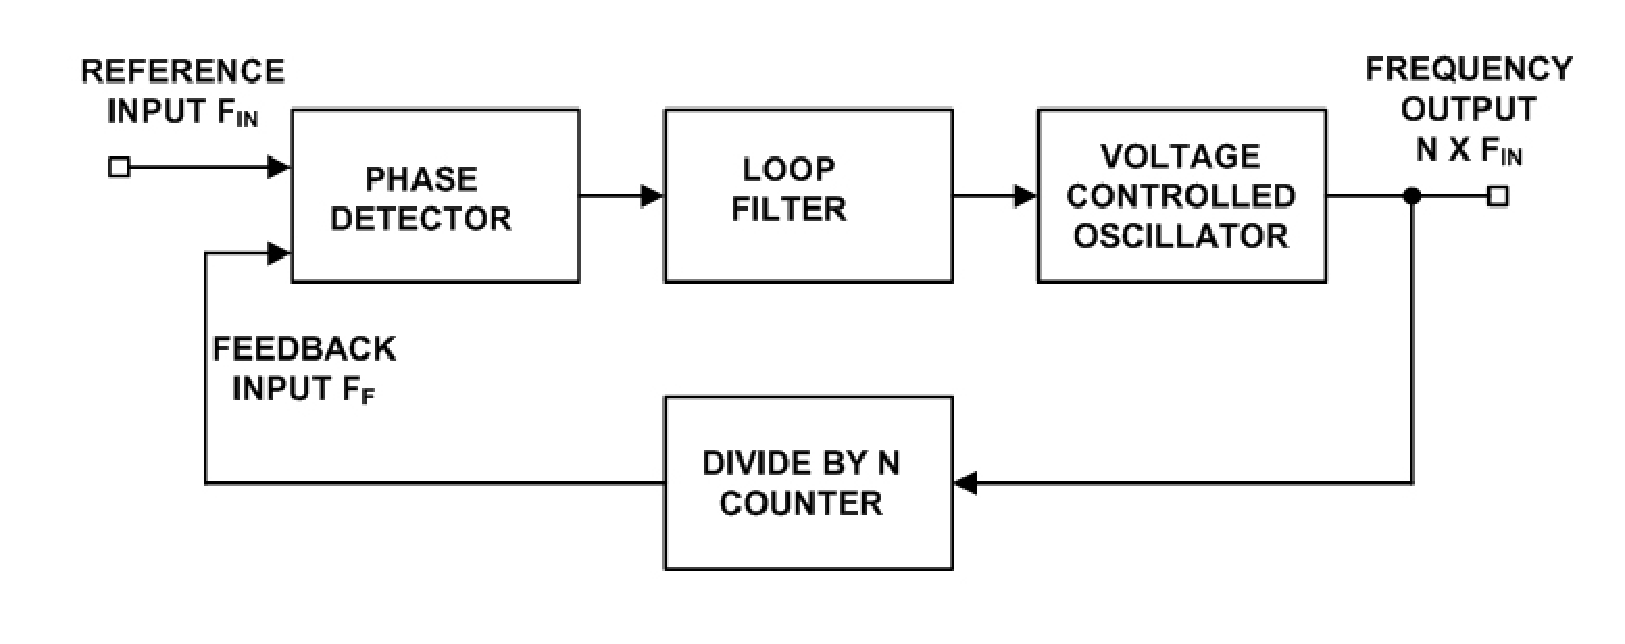
\includegraphics[width=0.65\textwidth]{./figures/pll.eps}
    \caption{ PLL
    \label{fig:pll2}}
\end{figure}

we can see that the output of the VCO is linearly related to the integral of the
control voltage.\\

Using laplace notation it is possible to stablish some basic equations to
describe the loop components behavior,

\begin{equation}
    V_d(s)=K_d[\theta_i(s) - \theta_o(s)]
    \label{eq:vd}
\end{equation}

\begin{equation}
    V_c(s)=F(s)V_d(s)
    \label{eq:vc}
\end{equation}

\begin{equation}
    \theta_o(s)=\frac{k_oV_c(s)}{s}
    \label{eq:thetao}
\end{equation}

The combination of these equations \ref{eq:vd}, \ref{eq:vc}, \ref{eq:thetao}
results in the basic loop equations:


\begin{equation}
    H(s)= \frac{\theta_o(s)}{\theta_i(s)}=
    \frac{K_oK_dF(s)}{s + K_oK_dF(s)}
    \label{eq:gentf}
\end{equation}

\begin{equation}
    \frac{\theta_i(s)-\theta_o(s)}{\theta_i(s)}=
    \frac{\theta_e(s)}{\theta_i(s)}=
    \frac{s}{s+K_oK_dF(s)}=1-H(s)
    \label{eq:pherr}
\end{equation}

\begin{equation}
    V_c(s)=\frac{sK_dF(s)\theta_i(s)}{s+K_oK_dF(s)}=
    \frac{s\theta_i(s)}{K_o}H(s)
    \label{eq:vchs}
\end{equation}

Where:

\begin{itemize}
    \item $H(s)$ is the closed-loop transfer function
    \item $\theta_e$ is the phase error
\end{itemize}

There is indeed another point to explore, regarding loop gain, the open-loop
transfer function (open-loop gain) of any PLL is,

\begin{equation}
    G(s)=\frac{K_oK_dF(s)}{s}
    \label{eq:olg}
\end{equation}

thus the closed-loop transfer function can be made in terms of \ref{eq:olg},

\begin{equation}
    H(s)=\frac{G(s)}{1+G(s)}
    \label{eq:clg}
\end{equation}

The DC gain can be defined as,

\begin{equation}
    K_v=K_oK_dF(0)
    \label{eq:dcgain}
\end{equation}

which has dimensions of frequency ($time^-1$). A high $K_v$ value is related to
a good performance of the loop. $F(s)$ is a rational function of the loop filter
in the form

\begin{equation}
    F(s)=\frac{g(s -z_1)(s-Z_2)\dots(s-z_m)}
    {(s-p_1)(s-p_2)(s-p_3)\dots(s-p_n-1)}
    \label{eq:filterrf}
\end{equation}

For the filter to be realizable m cannot exceed n-1, and if m=n-1 as often
occurs in PLL designs, then $g=F(\infty)$.

Expandign $F(s)$ in aprtial fractions it is possible to rewrite the open-loop
gain function as

\begin{equation}
    G(s)=\frac{K}{s}\Bigg[ a_1+\sum_{i=1}^{n-1} \frac{a_i+1}{s-p_i}\Bigg]
    \label{eq:gsfilter}
\end{equation}

where $K$ is the $loop gain$  and $a_1$ is zero if $m < n-1$, while $a_1 = 1$ 
if $m = n-1$, but K is only "defined" when $a_1 = 1$, thus the most important
PLLs are designed for $a_1 = 1$ (equal number of poles and zeroes in the loop
filter).

Based on the previous equations which describe the behavior of the components in the
phase-locked loop we can classify the pll based on the order of the transfer
function associated with the loop. This classification is based upon the nunmber
of perfect integrators ($\frac{1}{s}$) present in the transfer function.

\begin{itemize}
    \item First order loop.
    \item Second order loop.
    \item Third and higher order loop.
\end{itemize}

\subsubsection{First Order Loop}

The first order loop is the simplest implementation of a phase-locked loop,
where the loop filter is ommited, thus $F(s)=1$

\begin{equation}
    H(s)= \frac{K_oK_d}{s + K_oK_d}=
    \frac{K}{s + K}
    \label{eq:tf1st}
\end{equation}

Where:
\begin{itemize}
    \item $K = K_oK_d =K_v$;
\end{itemize}

In the first-order loop the only parameter avaible to the designer is the loop
gain

\subsubsection{Second Order Loop}

In the second order loop the loop filter is used and it is possible to separate
it in two major "classes", the loop which use passive filters and the loops
whose use active filters. The loops which use passivel filters require high-gain
DC amplifier but provides good tracking performance, the closed-loop transfer
function for a passive filter is

\begin{equation}
    H_1(s)=\frac{K_oK_d(s\tau_2+1)/\tau_1}
    {s^2+s(1+K_oK_d\tau_2)/\tau_1+K_oK_d/\tau_1}
    \label{eq:tf2ndpass}
\end{equation}

and for rthe active filter the closed-loop trasnfer function is

\begin{equation}
    H_2(s)= \frac{K_oK_d(s\tau_2+1)/\tau_1}
    {s^2+s(1+K_oK_d\tau_2)/\tau_1+K_oK_d/\tau_1}
    \label{eq:tf2ndact}
\end{equation}

witha very large amplifier gain \ref{eq:tf2ndpass} and \ref{tf2ndact} can be 
rewritten as

\begin{equation}
    H_1(s)= \frac{s(2\zeta\omega_n-\omega_n^2/K_oK_d)+\omega_n^2}
    {s^2+2\zeta\omega_ns+\omega_n^2}
    \label{eq:damph1}
\end{equation}

\begin{equation}
    H_1(s)= \frac{2\zeta\omega_ns+\omega_n^2}
    {s^2+2\zeta\omega_ns+\omega_n^2}
    \label{eq:damph2}
\end{equation}

where $\omega_n$ is the natural frequency of the loop and $\zeta$ is the damping
factor.\\

The second-order loops are the most prevalent used loop but depending on the
application another loop orders are required.

\subsubsection{Third Order Loops}

As stated before, depending on the situation the third-order loop is necessary
because it can track a frequency ramp with zero steady error for example. The
basic setup of a third order PLL is when the two poles of the filter are at the
origin, that is, if the loop filter has two cascated integrators, so the closed
loop transfer function is

\begin{equation}
    H(s)=\frac{K(s^2+a_2s+a_3)}{s^3+K(s^2+a_2s+a_3)}
    \label{eq:tf3rd}
\end{equation}

it is rare to see a loop built with an order higher than 3, because as the order
raises the more difficult it is to stabilize the loop and it gets more sensitive
to to changes in the gain circuit components.

\subsubsection{Analysis Tools}
There are two main ways to analyse the behavior of a phase-locked loop one of
them is the root-locus plot which can be built by determining the locations of
the poles of the closed-loop response, these poles change their location as the
gain is changed throught the s-plane. The root-locus plot is used to show these
paths and can be easily obtained by following a few simple rules.(appendice root
locus)

\begin{figure}[htbp]
    \centering
    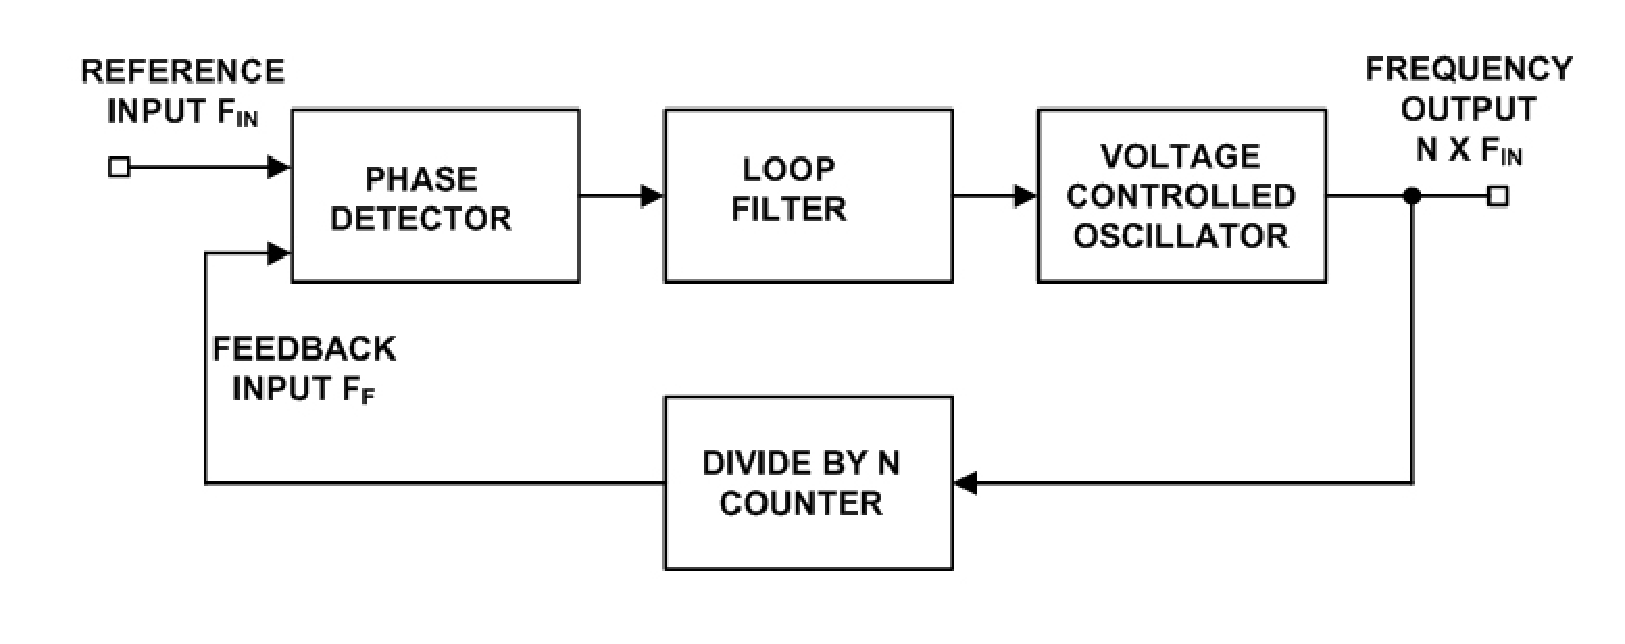
\includegraphics[width=0.65\textwidth]{./figures/pll.eps}
    \caption{ Root-Locus plot for a first-order PLL
    \label{fig:rlocus1}}
\end{figure}

\begin{figure}[htbp]
    \centering
    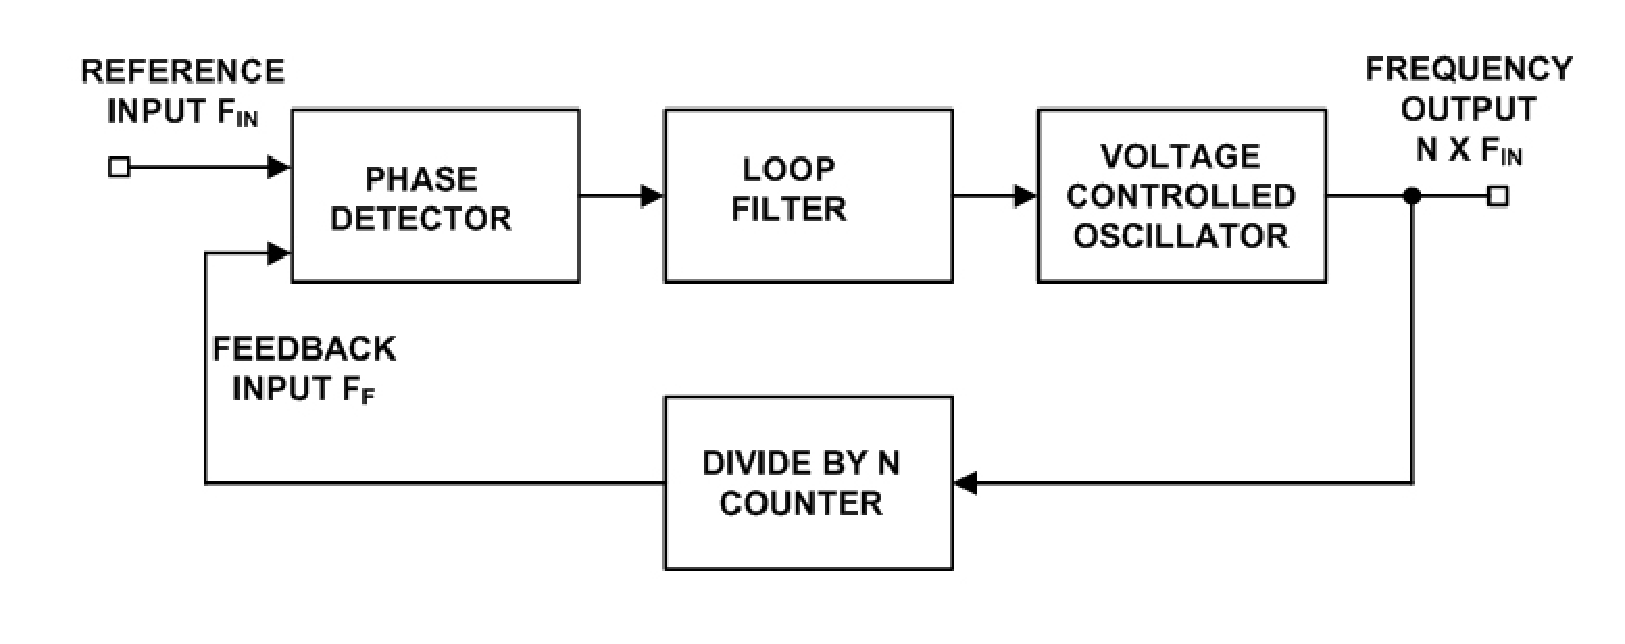
\includegraphics[width=0.65\textwidth]{./figures/pll.eps}
    \caption{ Root-Locus plot for a second-order PLL
    \label{fig:rlocus2}}
\end{figure}

\begin{figure}[htbp]
    \centering
    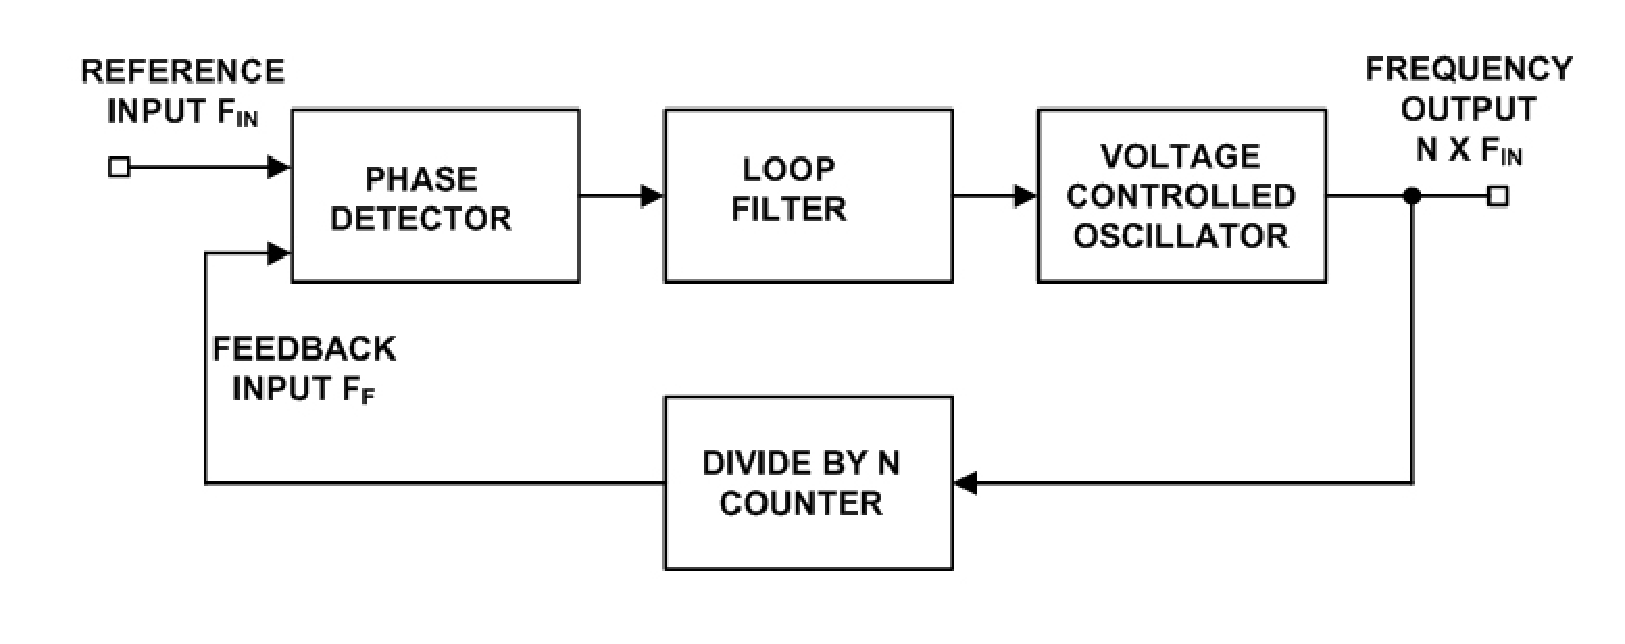
\includegraphics[width=0.65\textwidth]{./figures/pll.eps}
    \caption{ Root-Locus plot for a third-order PLL
    \label{fig:rlocus3}}
\end{figure}

Another useful tool is the Bode plot (apendice bode plot), which is a pair of
curves displaying the polar components of $G(j\omega)$.

\begin{figure}[htbp]
    \centering
    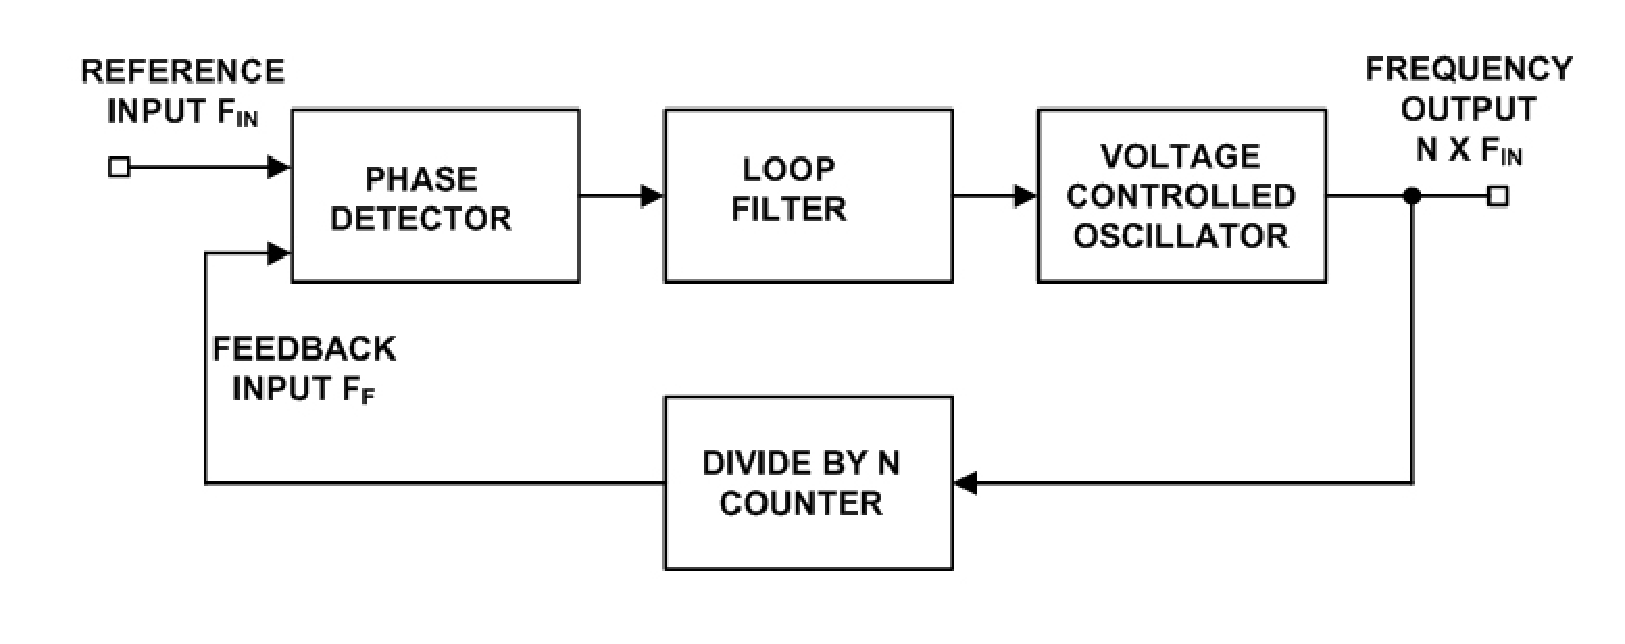
\includegraphics[width=0.65\textwidth]{./figures/pll.eps}
    \caption{ Root-Locus plot for a third-order PLL
    \label{fig:rlocus3}}
\end{figure}

\begin{figure}[htbp]
    \centering
    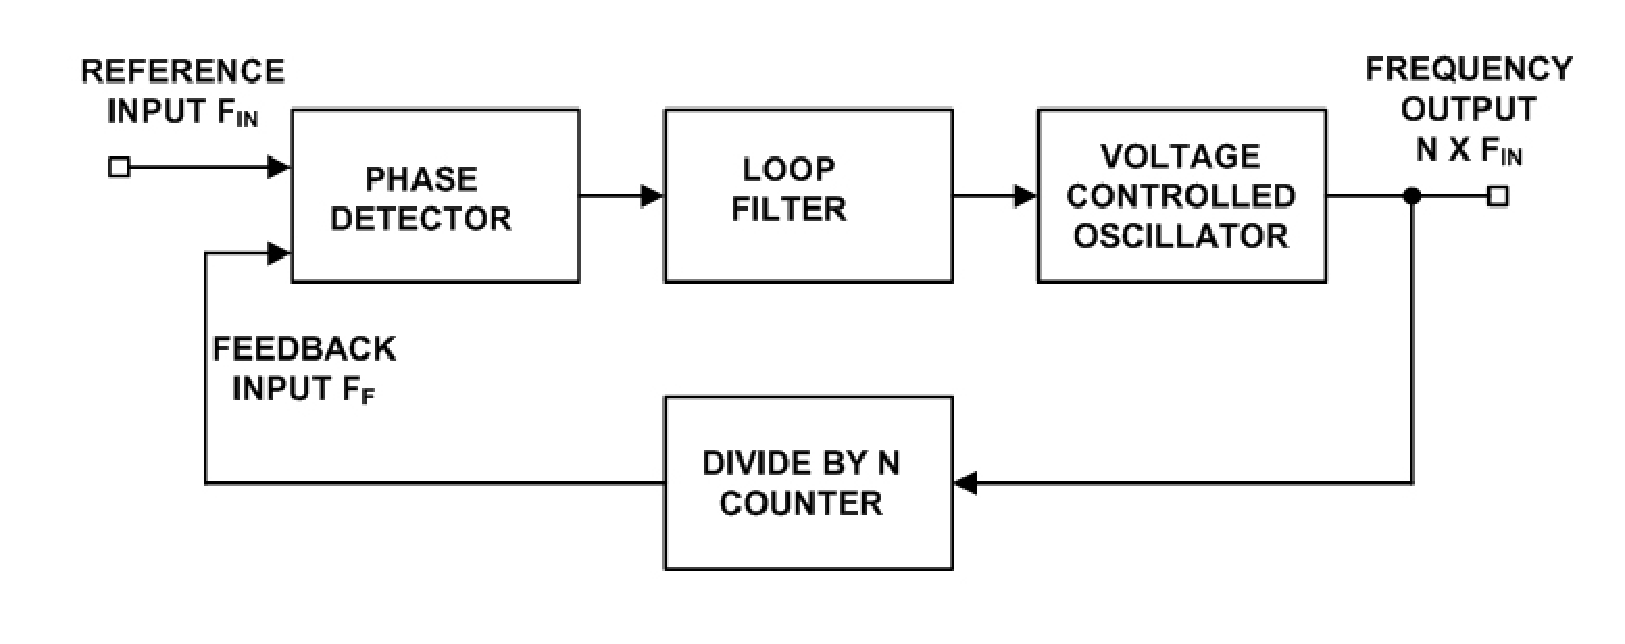
\includegraphics[width=0.65\textwidth]{./figures/pll.eps}
    \caption{ Root-Locus plot for a third-order PLL
    \label{fig:rlocus3}}
\end{figure}

\begin{figure}[htbp]
    \centering
    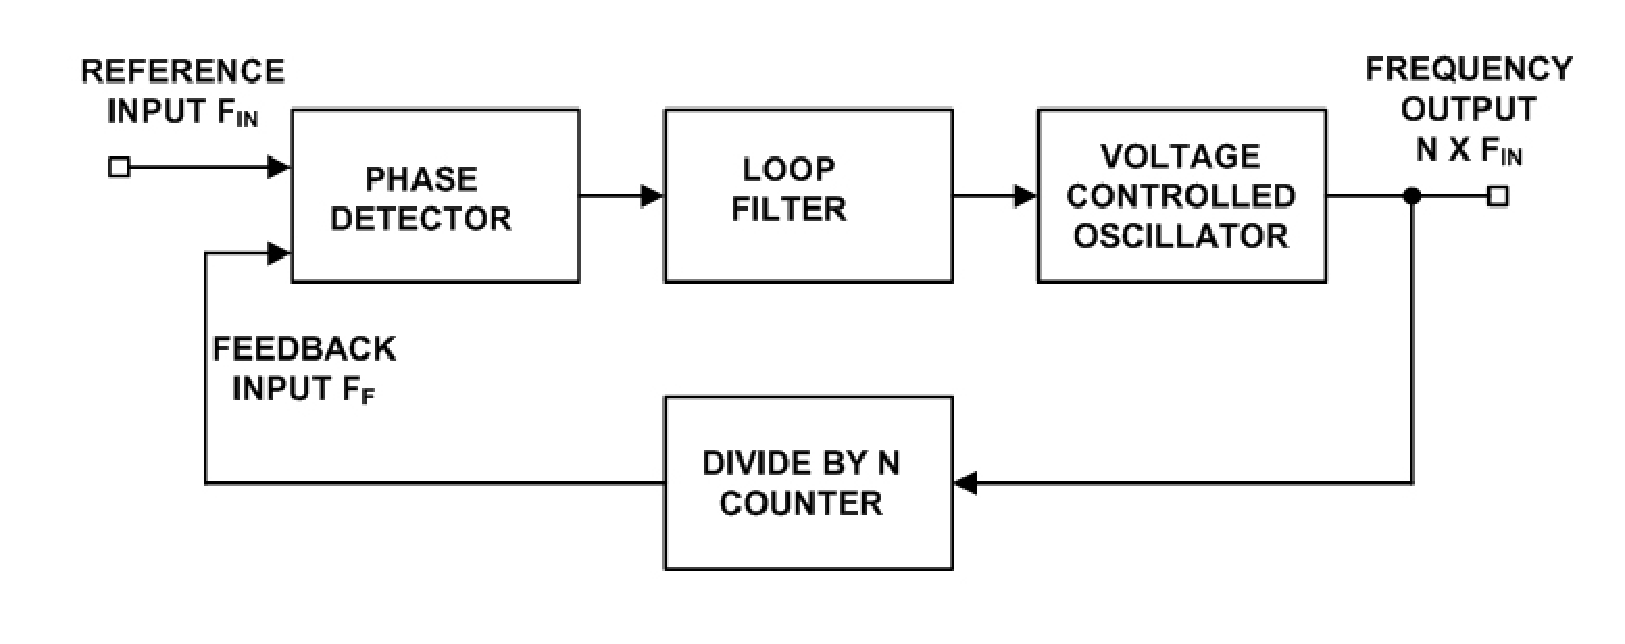
\includegraphics[width=0.65\textwidth]{./figures/pll.eps}
    \caption{ Root-Locus plot for a third-order PLL
    \label{fig:rlocus3}}
\end{figure}

\begin{figure}[htbp]
    \centering
    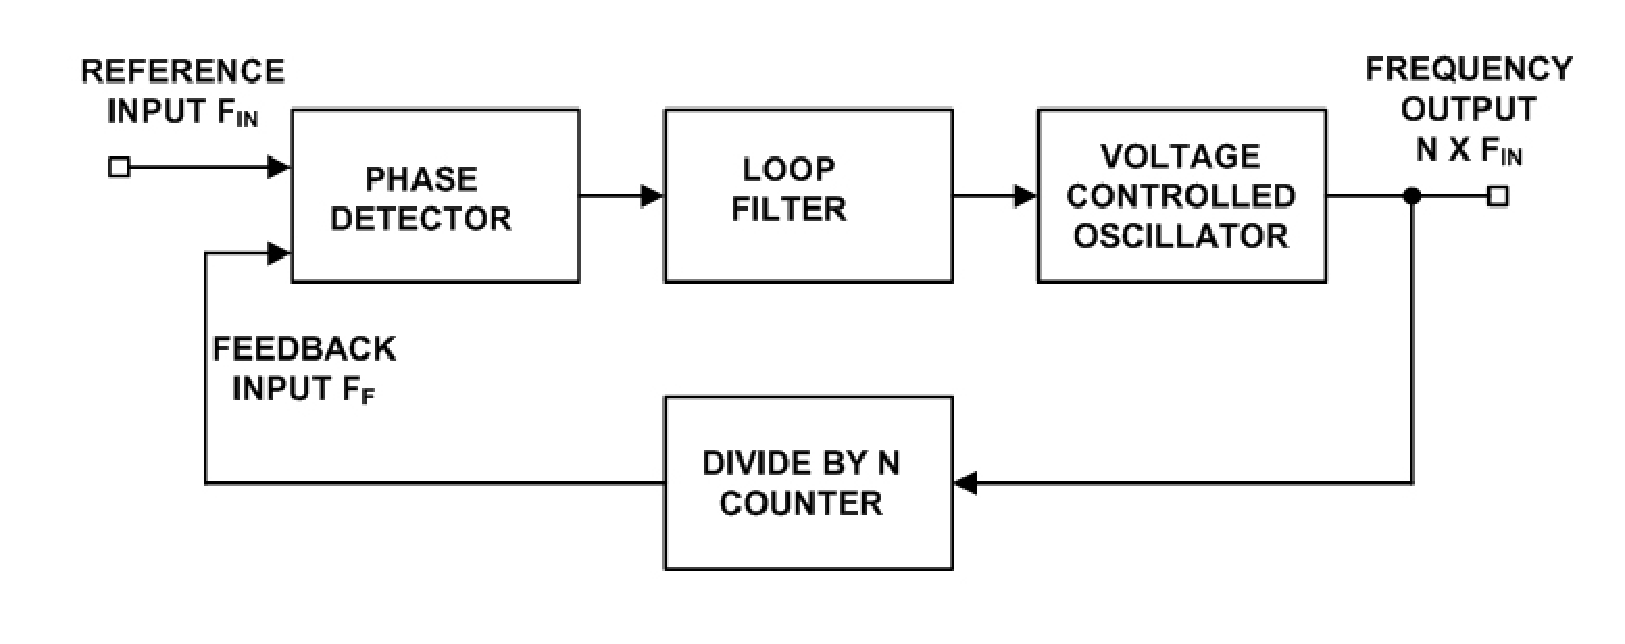
\includegraphics[width=0.65\textwidth]{./figures/pll.eps}
    \caption{ Root-Locus plot for a third-order PLL
    \label{fig:rlocus3}}
\end{figure}

\subsection{PLL Components}
As stated in the beginning of this section and as can be seen in the figure
\ref{fig:pll} the elementary Phase-locked Loop is composed of three main 
components, the phase detector, the loop filter and the voltage-controlled 
oscillator. This subsection aims in introducting the basic components and any
useful theory.

\subsubsection{Loop Filter}

\subsubsection{Voltage-Controlled Oscillator}

\subsubsection{Phase-Detector}

\subsection{Linearized Analogic PLL Tracking}
Since the scope of this work is not PLL itself the nonlinear behavior will not
be explored here, all the assumptions in this subsection shall be of linearized
loops.\\
To understand tracking it is necessary to understand the PLL behavior until it
locks and consequently the noise behavior of the PLL is also an important
matter.\\
\subsubsection{Noise Behavior}


\subsection{Modulation and Demodulation using PLL}

\subsection{Discrete-time PLL}

\subsection{Design of PLL and DPLL}

\subsection{Costas Loop}


\part{Implementation}
\chapter{Radio Frontend Description}
The focus of this work will be the radio frontend interface, and using the 
fmcomms2 

\section{FmcommS2}



\chapter{FPGA}
\section{ML605 - Virtex6}
\section{VC707 - Virtex7}

\chapter{Setup Description}


\section{Overview}

\section{Integration between FPGA and FMComms2}

\part{Final Results}
\chapter{Results}
\label{chap:results}

This works goals were divided in basically three steps, configuration, transmission
and reception, having these three steps barely working it is possible to make a
transmission and analyze data. It is possible to see in figure \ref{fig:setup}
how the hardware is arranged and in figure \ref{fig:setupbd} it is possible to
behold the setup's block diagram, which gives the idea of the complexity behind
the design and how each component is connected.

%foto setup pronto
\begin{figure}[htbp]
    \centering
    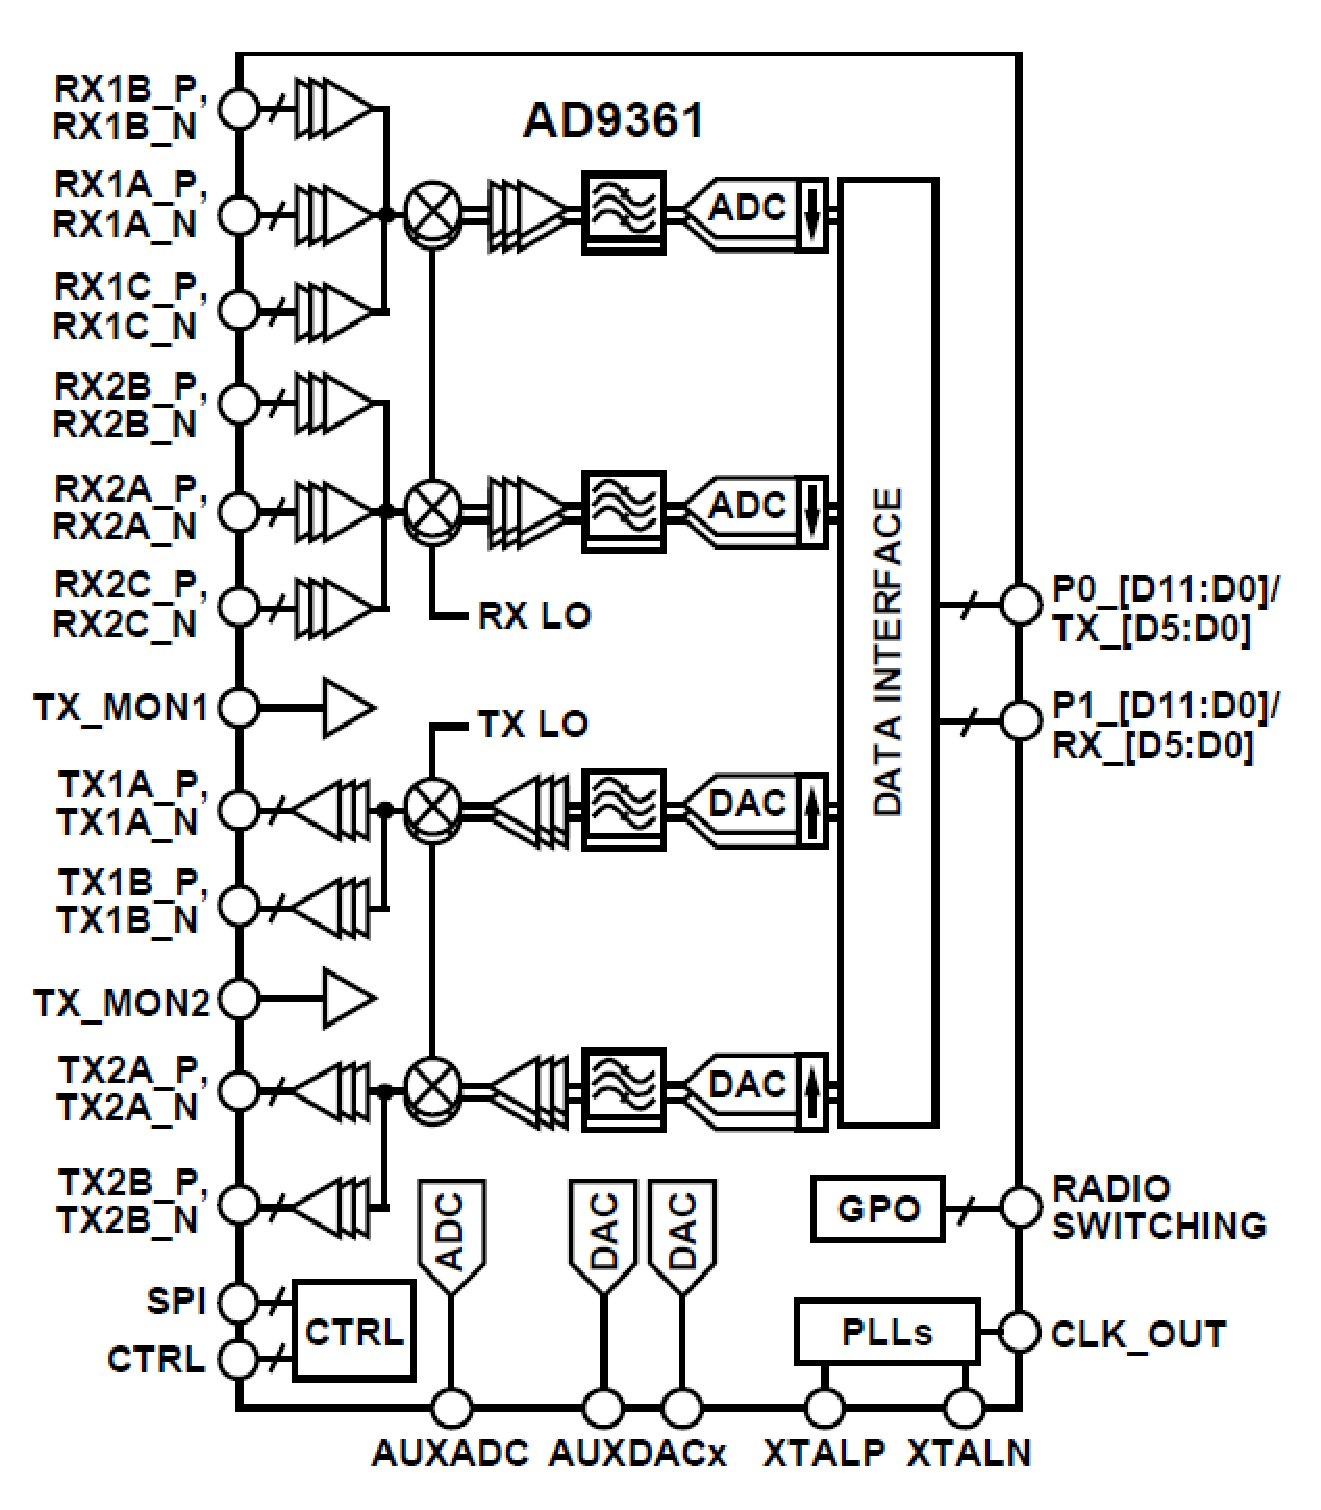
\includegraphics[width=0.45\textwidth]{./figures/ad9361_functional_diagram}
    \caption{ Image of the Setup Hardware
    \label{fig:setup}}
\end{figure}

\begin{figure}[htbp]
    \centering
    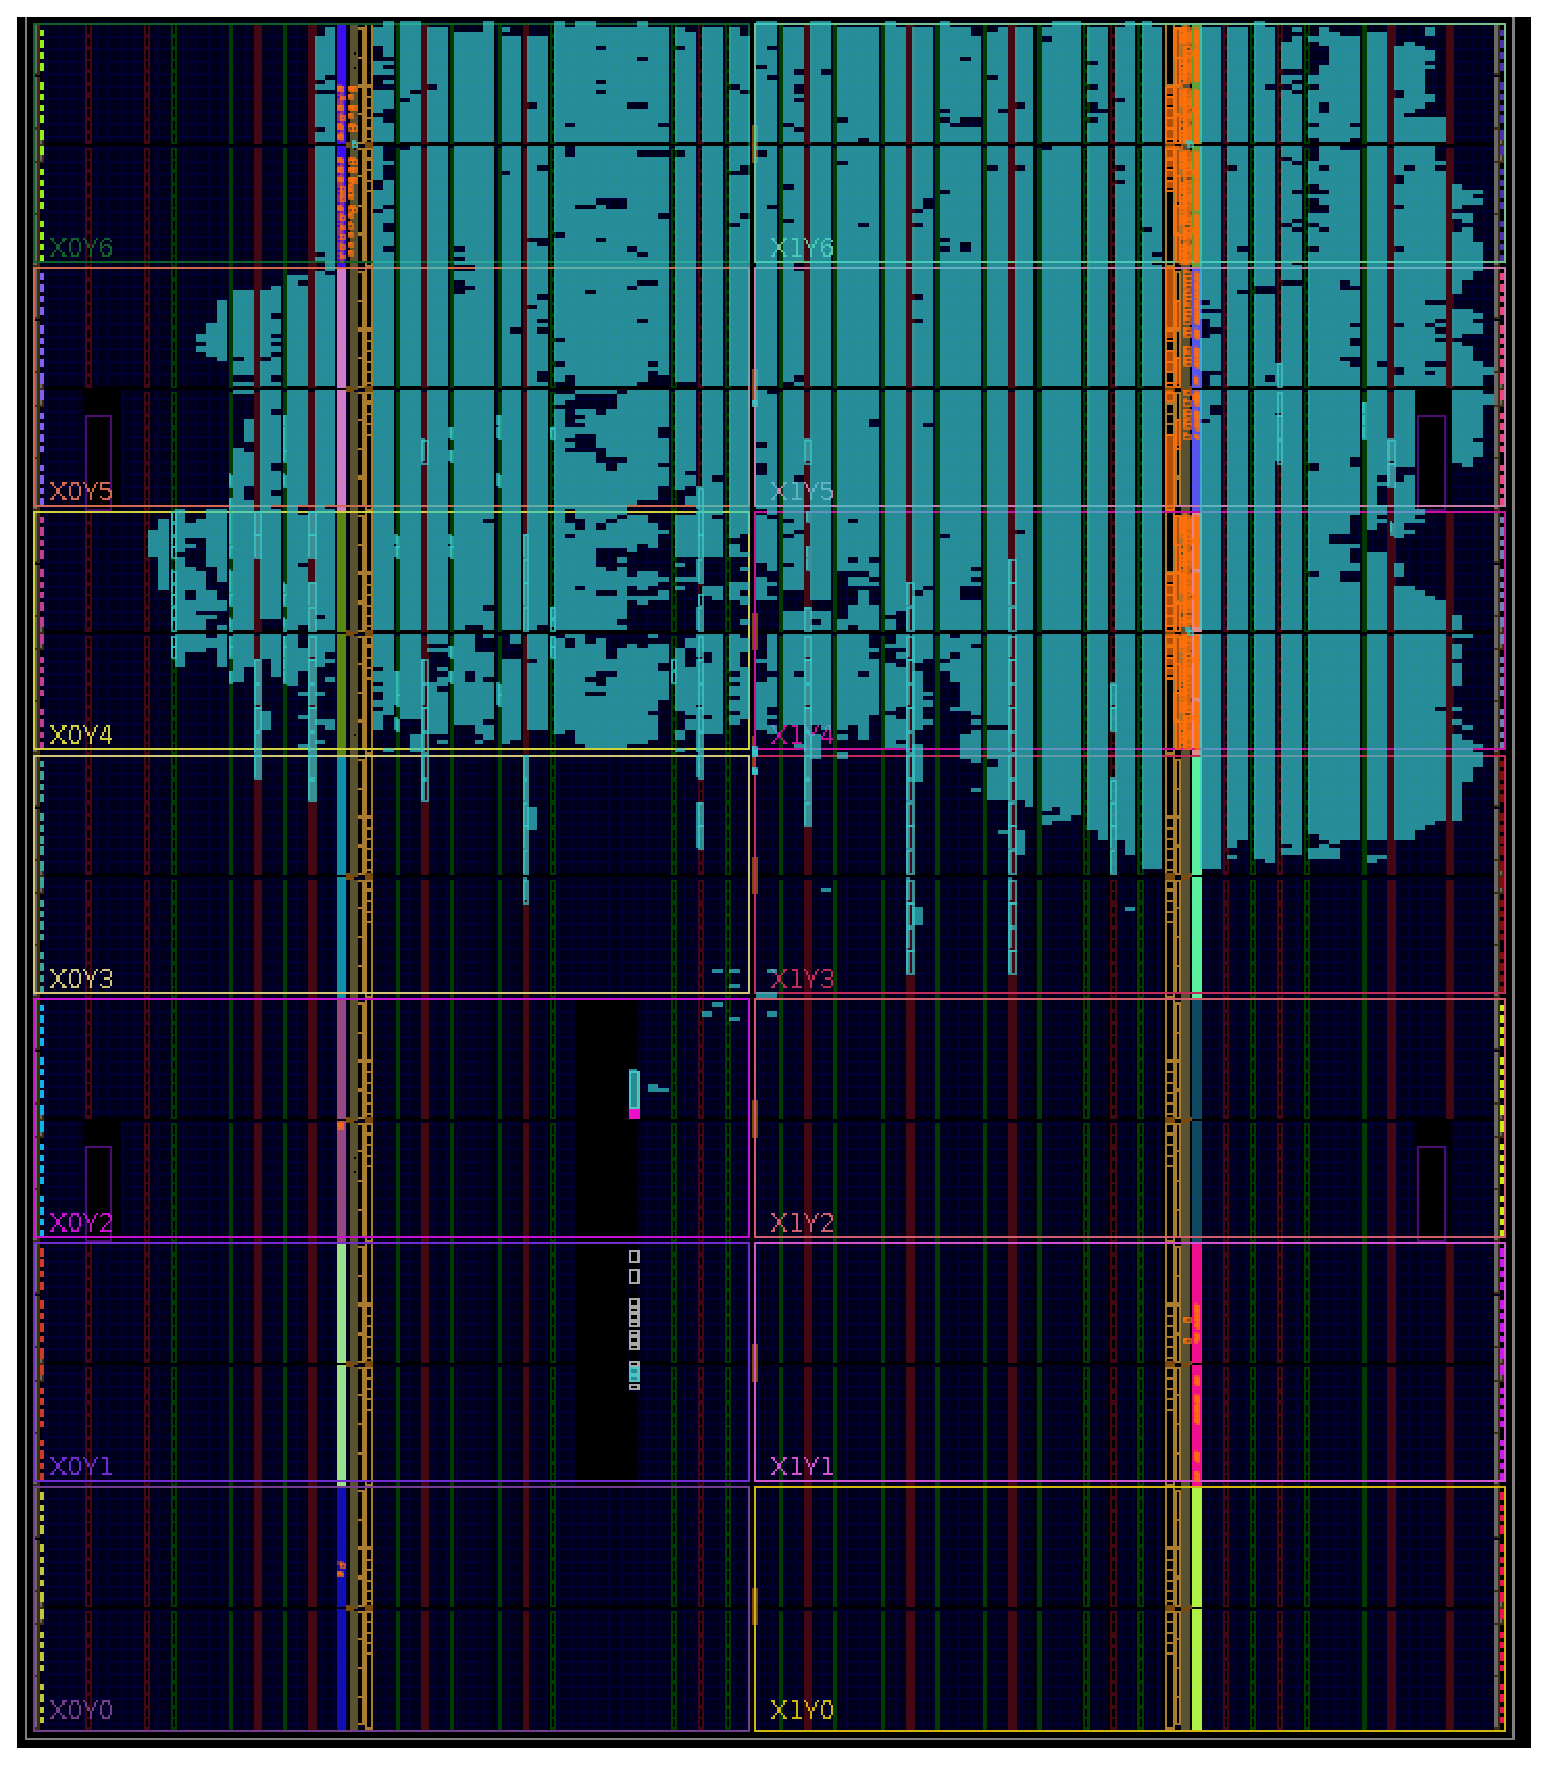
\includegraphics[width=0.35\textwidth]{./figures/fpga_area}
    \caption{ FPGA area used in this Setup
    \label{fig:fpgaarea}}
\end{figure}

%foto diagrama de blocos
\begin{figure}[htbp]
    \centering
    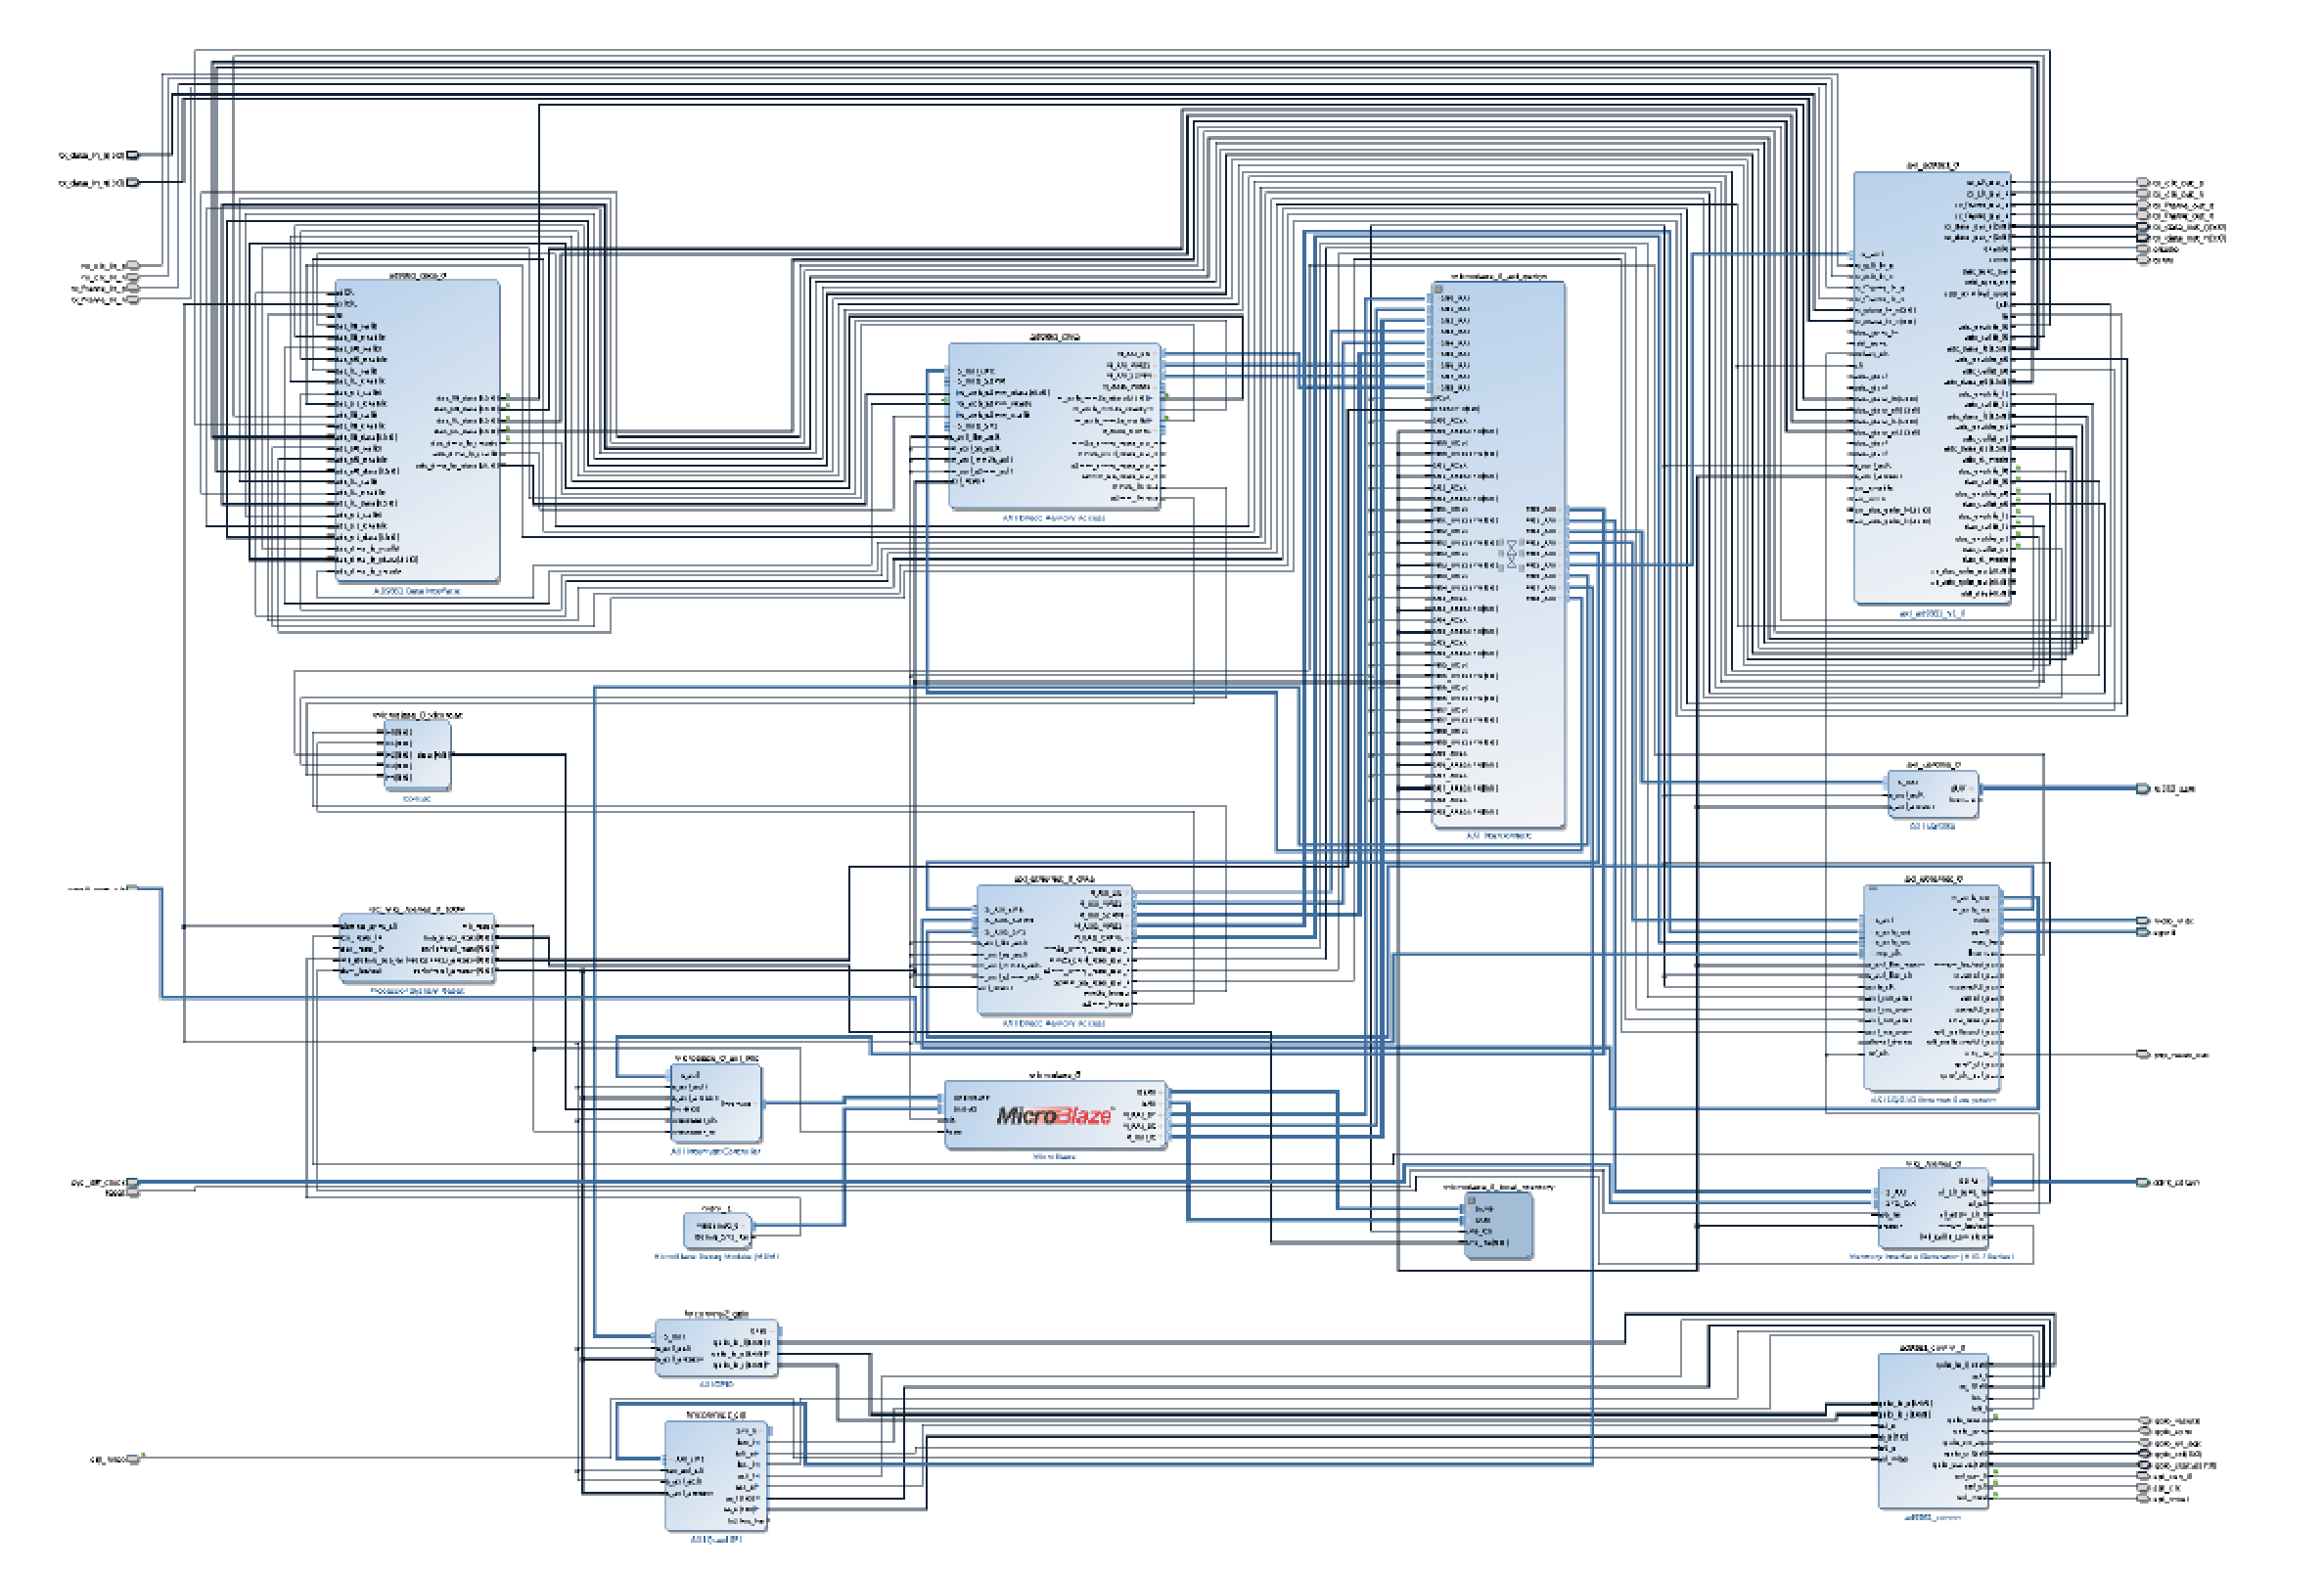
\includegraphics[width=0.95\textwidth]{./figures/setup_bd}
    \caption{ Image of the Setup Block diagram
    \label{fig:setupbd}}
\end{figure}

\vfill
\clearpage

\section{Preliminary Tests}
\label{result:conf}

The preliminary tests were focusing on initializing and communication between FPGA
and the FMComms2 board, in the previous chapter the steps of setting up communication
and control interface were described, and it describes also how this interface works
and how a block was made to implement such, in short it was needed to set up SPI and GPIO
modules and make the right input and output ports specified in \ref{subs:controlif} and
after the initialization and callibration is finished, it is possible to observ the
carrier wave centralized at the frequency 2.4 Ghz.

To generate the outputs two analyzers were used, one oscilloscope and one spectrum analyzer,
both analyzers outputs can be seen in the figures below:

%spectrum analyser image
\begin{figure}[htbp]
    \centering
    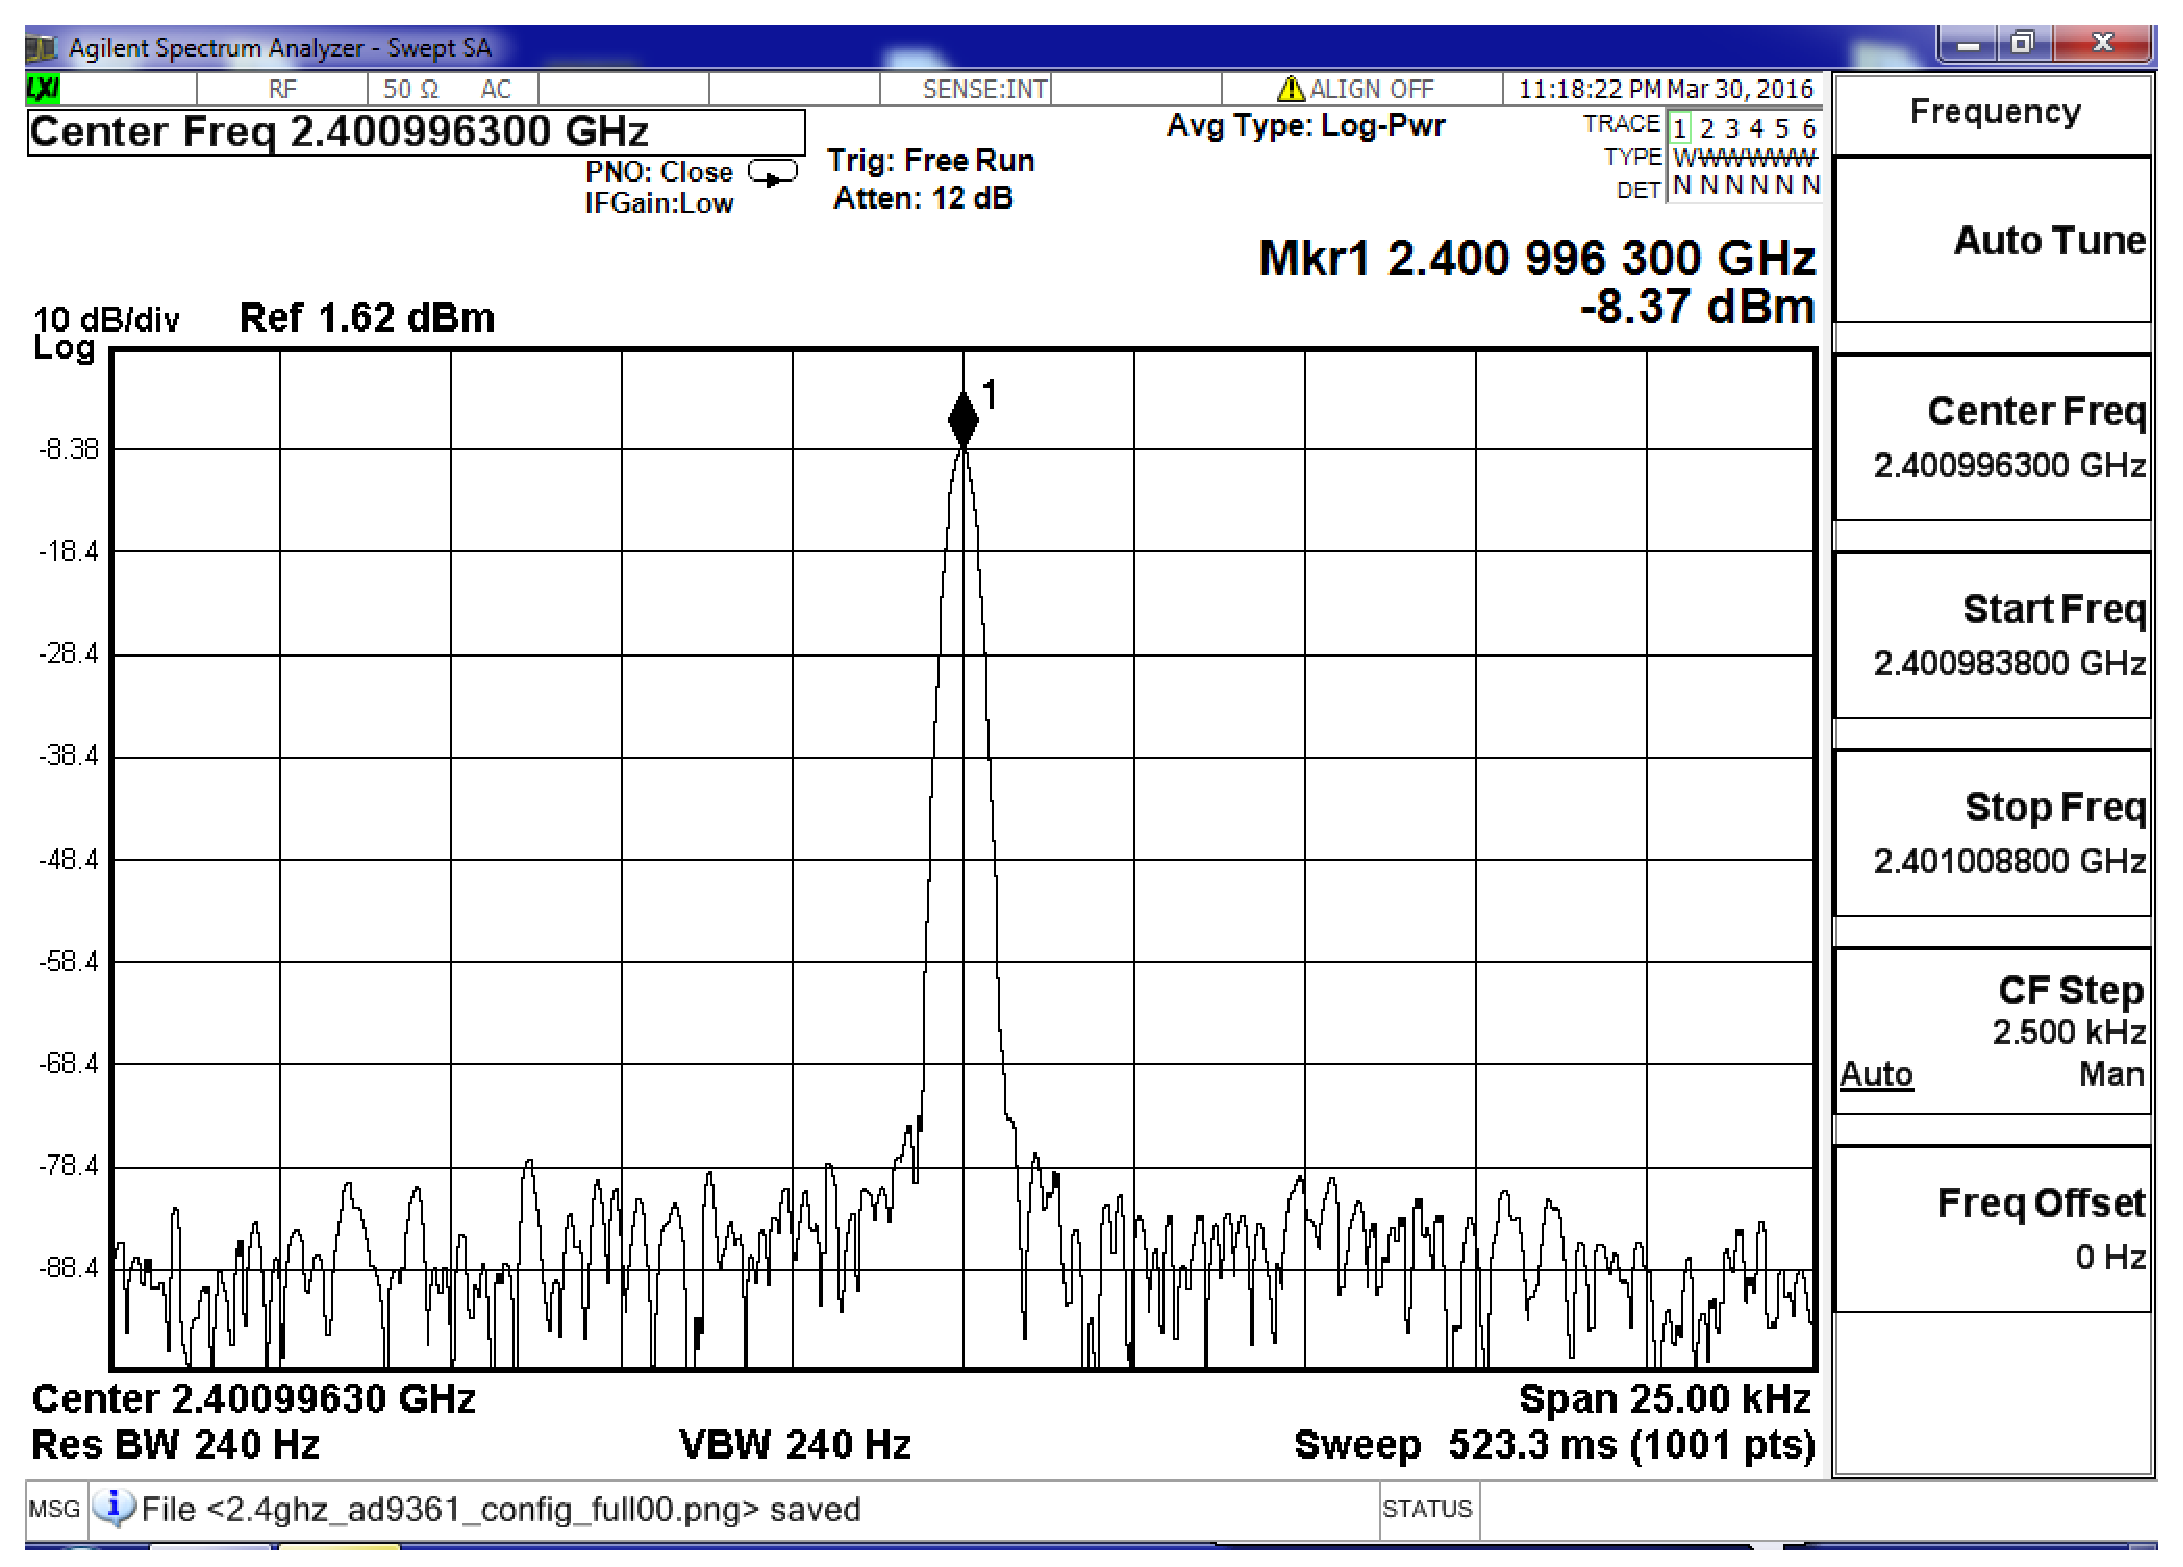
\includegraphics[width=0.85\textwidth]{./figures/spectrum_init}
    \caption{ Spectrum Analyzer Screen
    \label{fig:spec}}
\end{figure}

%initialization
\begin{figure}[htbp]
    \centering
    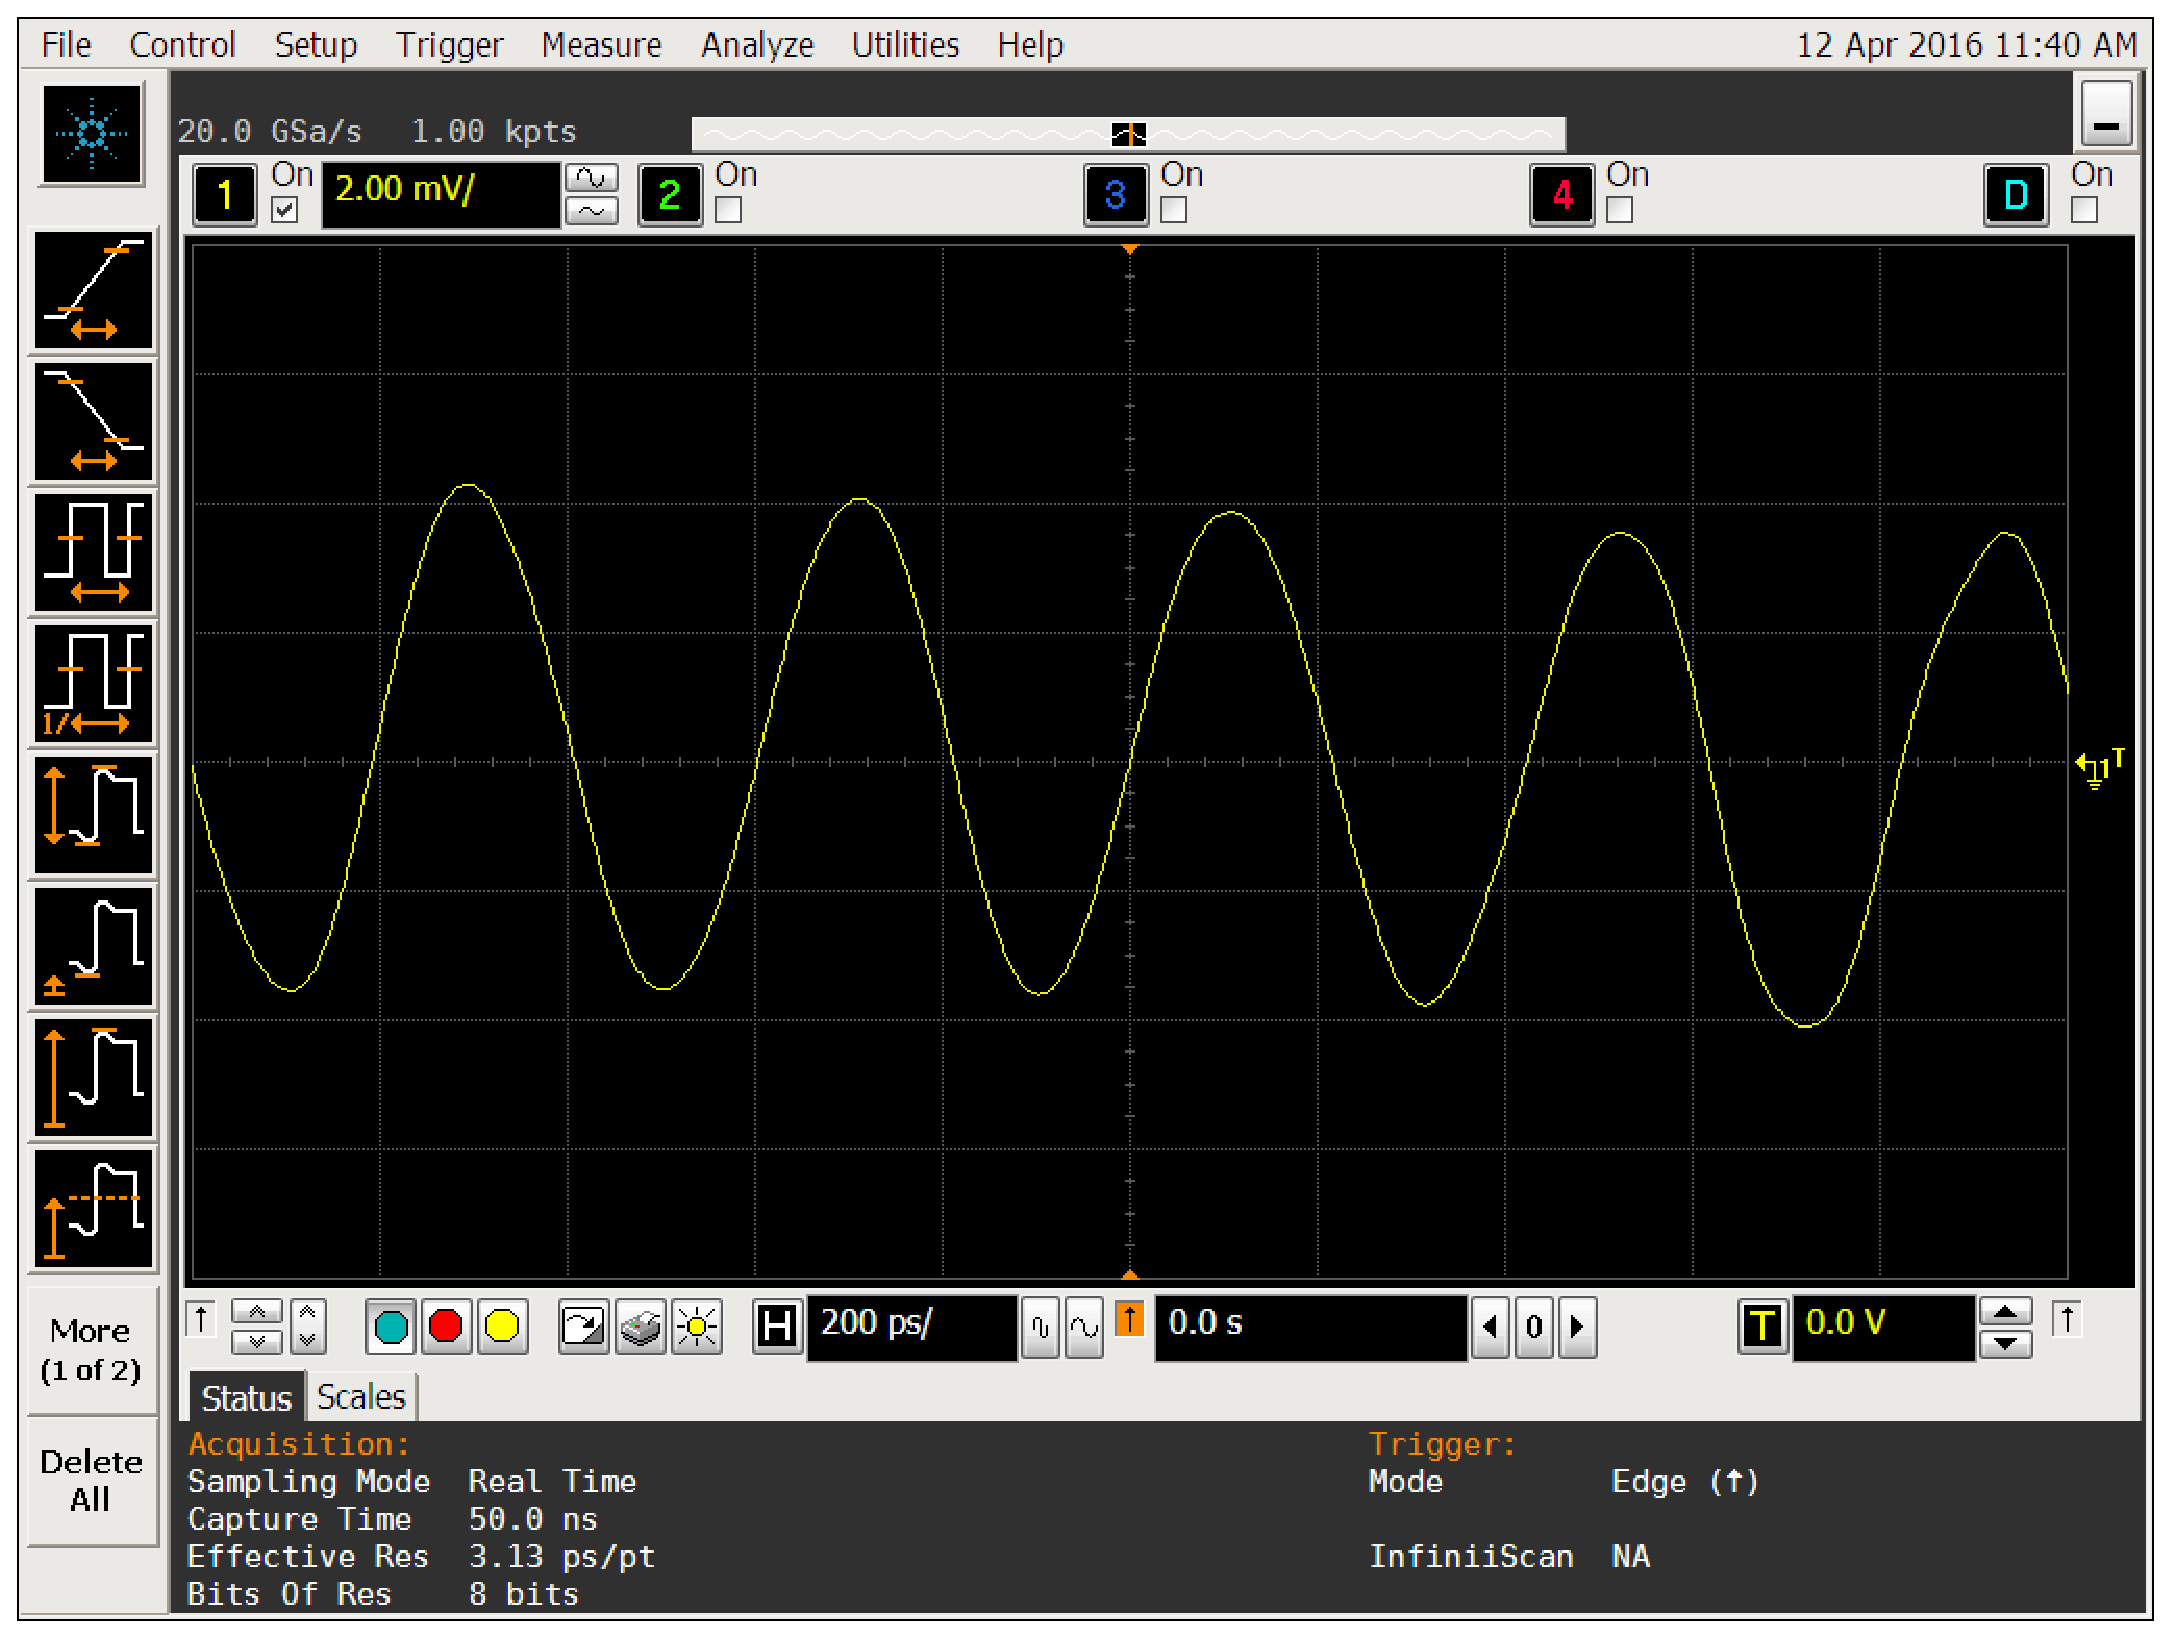
\includegraphics[width=0.85\textwidth]{./figures/oscill_init}
    \caption{ Carrier Waveform after Initialization
    \label{fig:oscillinit}}
\end{figure}

%digital tune
\begin{figure}[htbp]
    \centering
    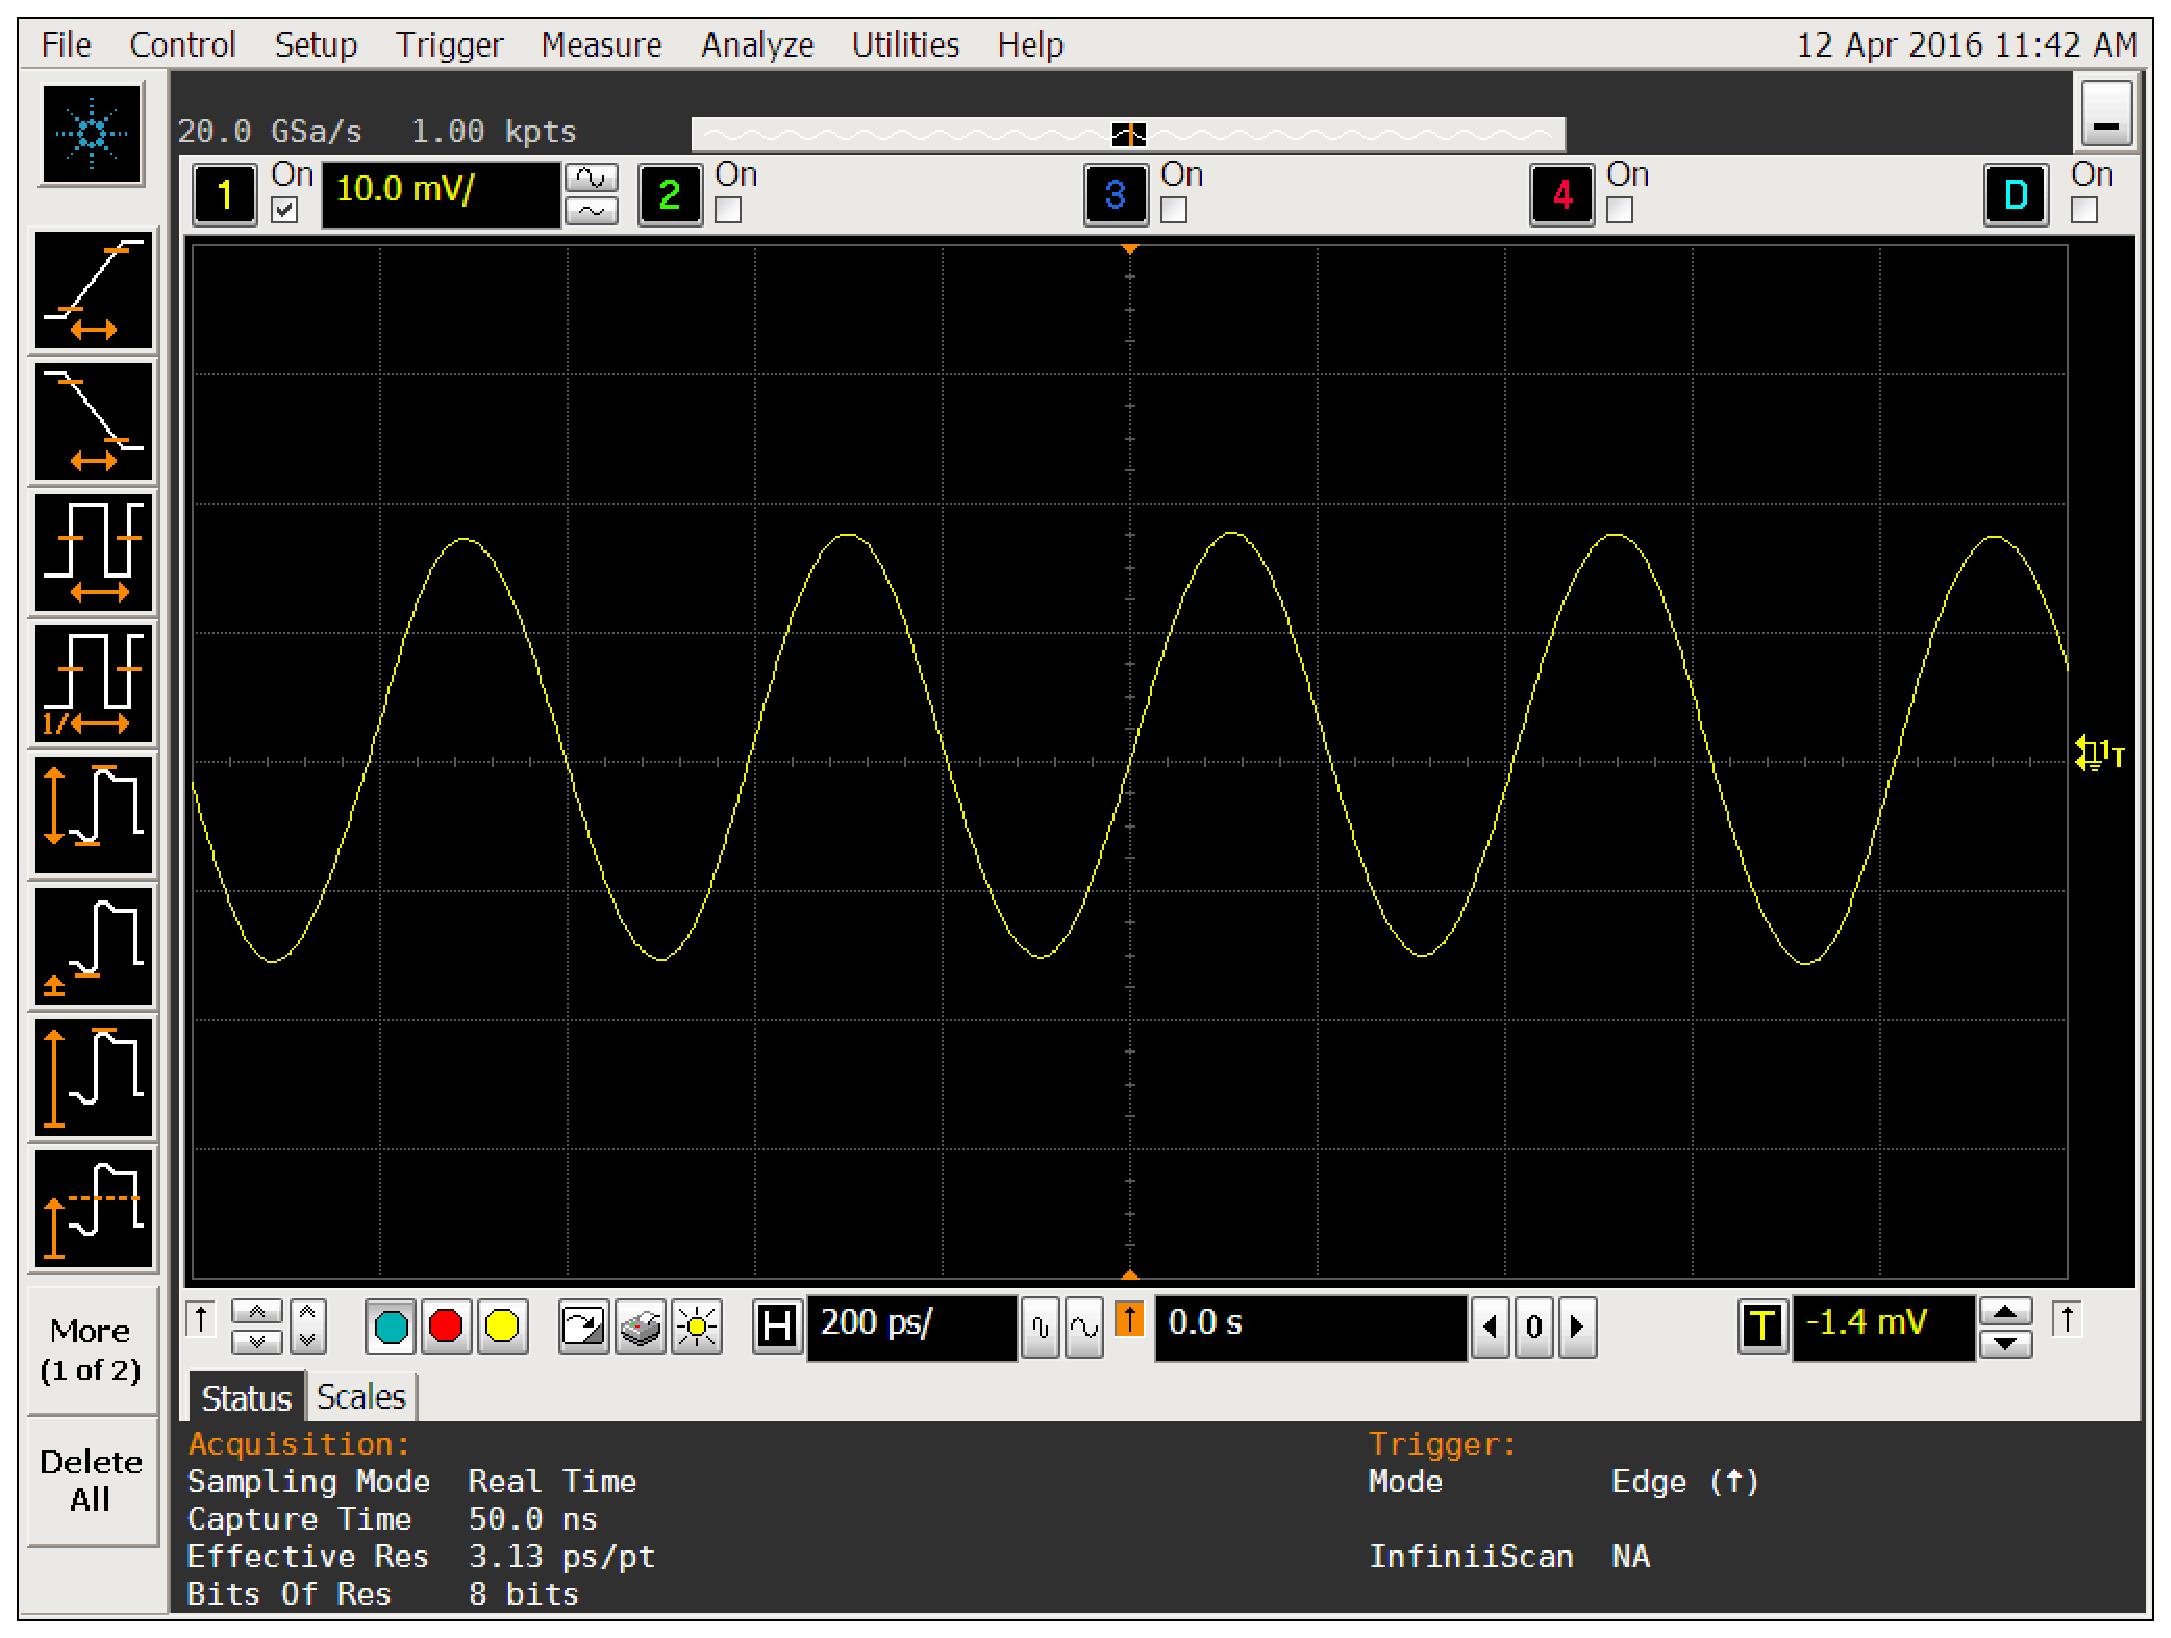
\includegraphics[width=0.85\textwidth]{./figures/oscill_dig}
    \caption{ Carrier Waveform after Tunning Digital Interface
    \label{fig:oscilldig}}
\end{figure}

%freq
\begin{figure}[htbp]
    \centering
    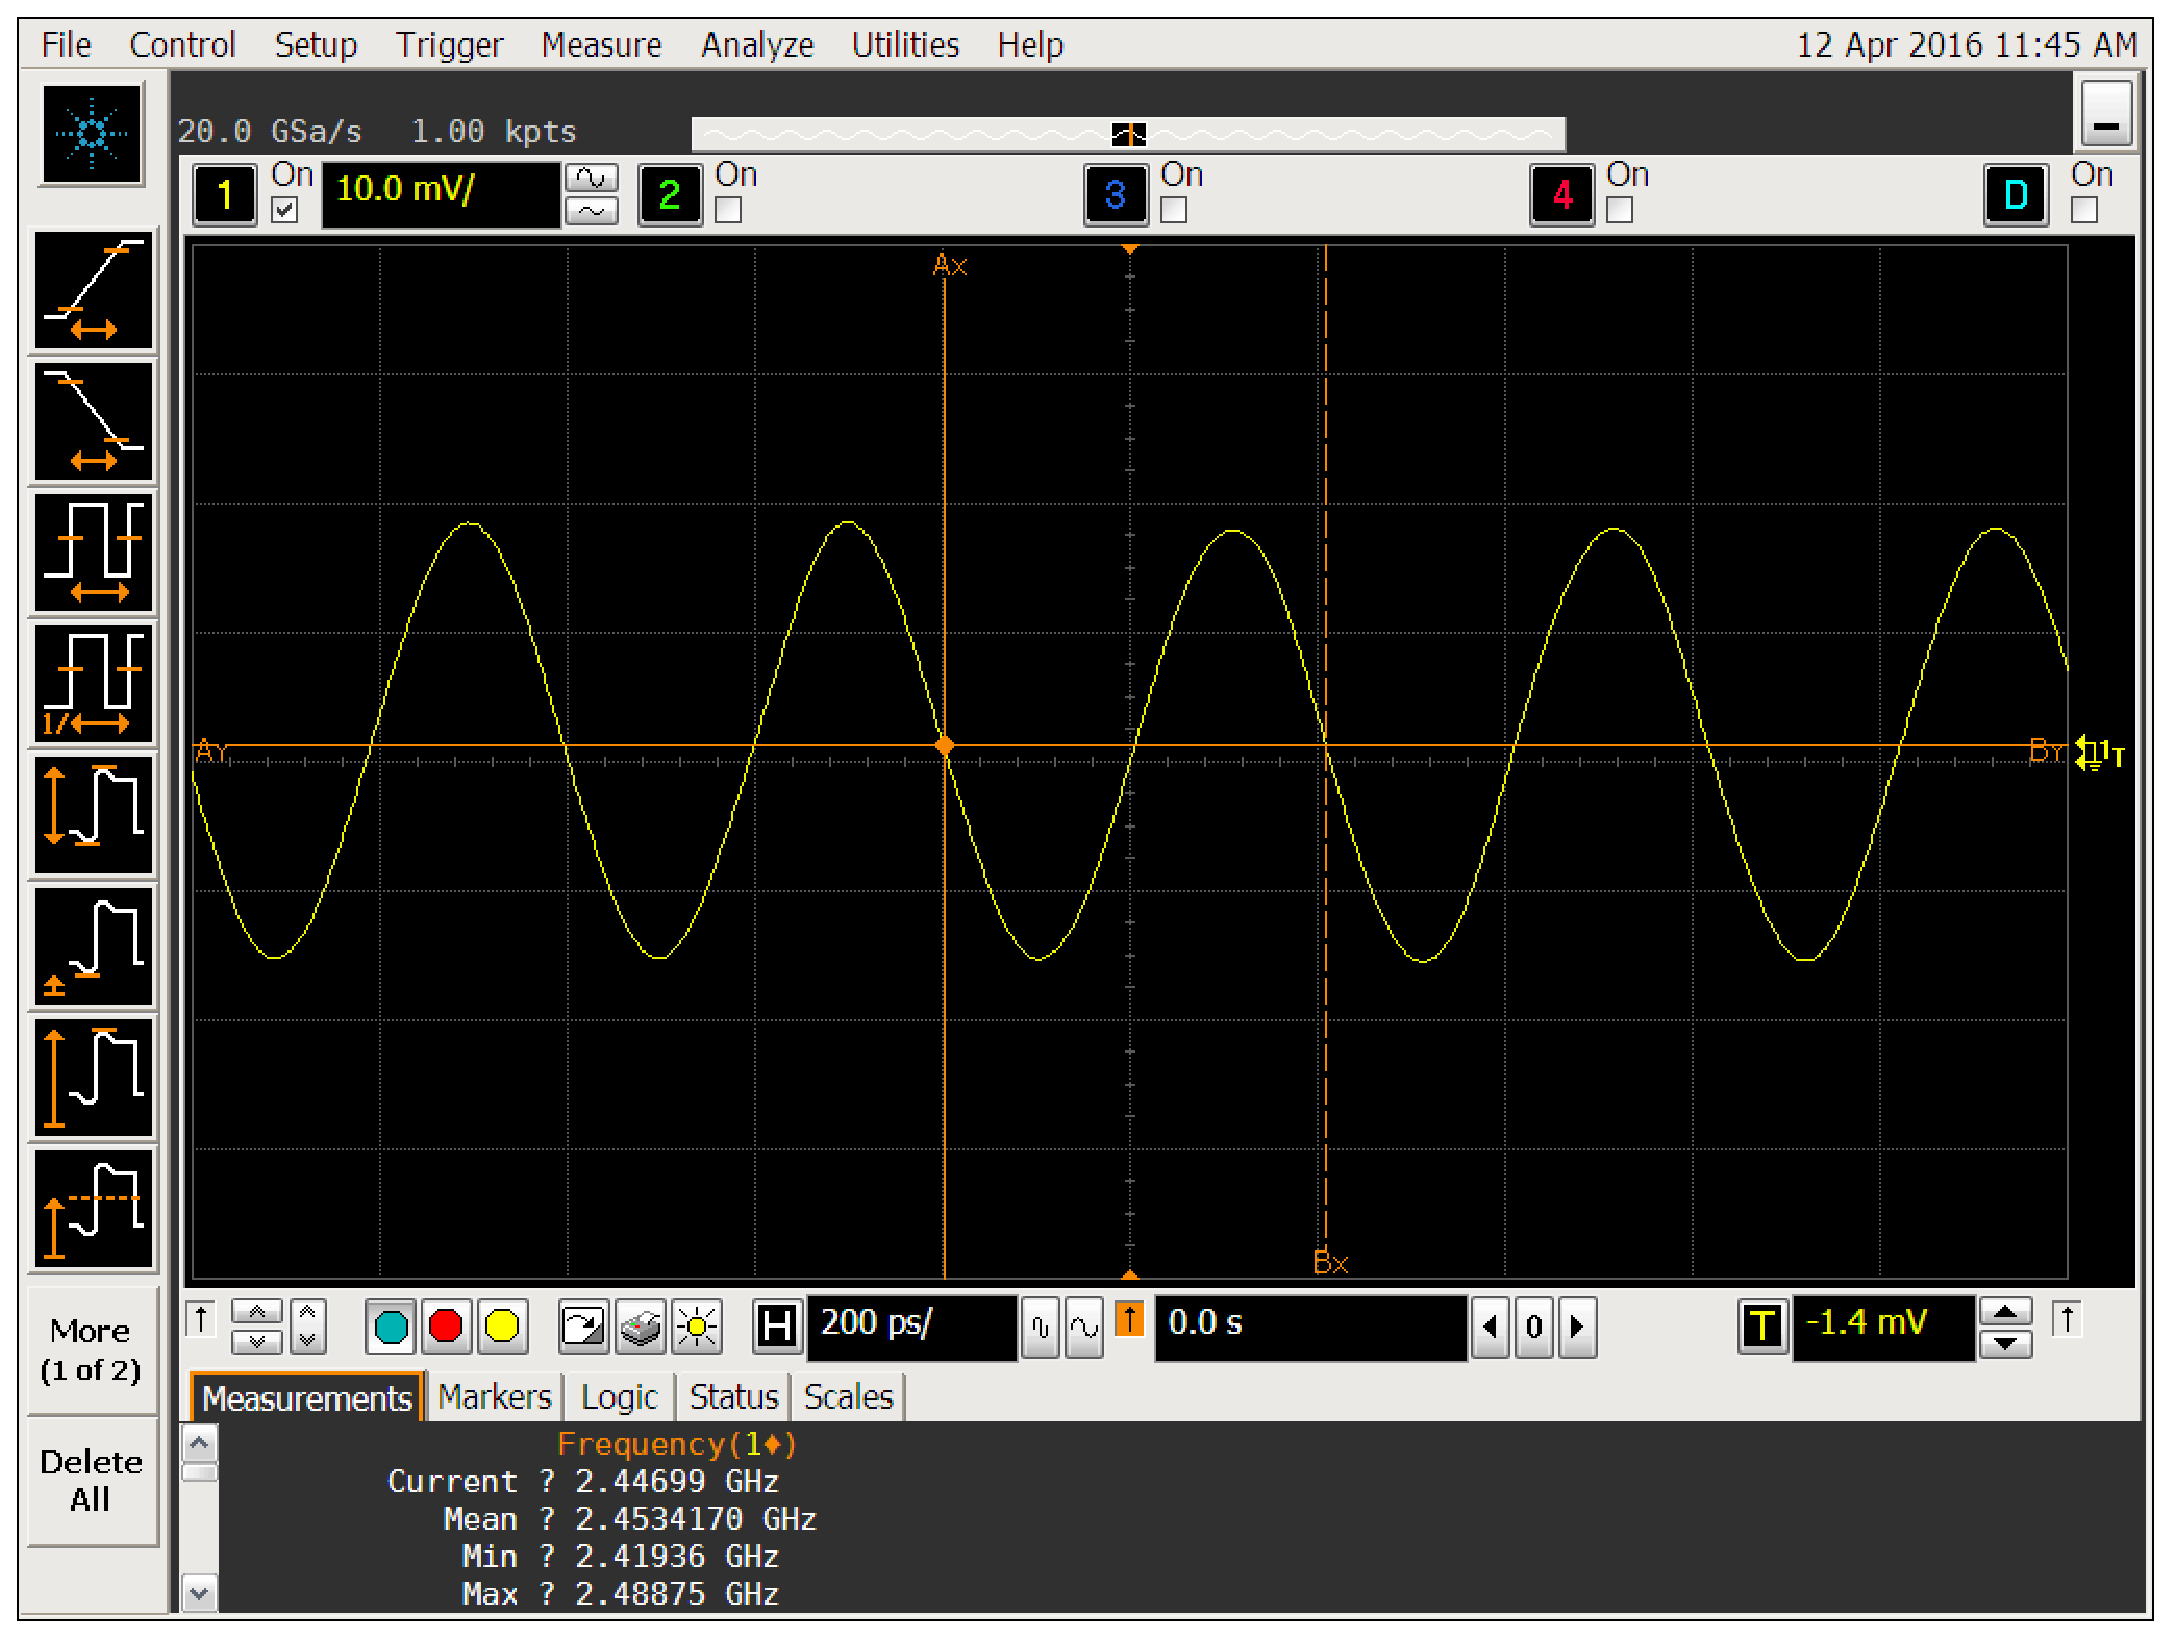
\includegraphics[width=0.85\textwidth]{./figures/oscill_freq}
    \caption{ Carrier Waveform with Frequency Measure
    \label{fig:oscillfreq}}
\end{figure}

%fft config
\begin{figure}[htbp]
    \centering
    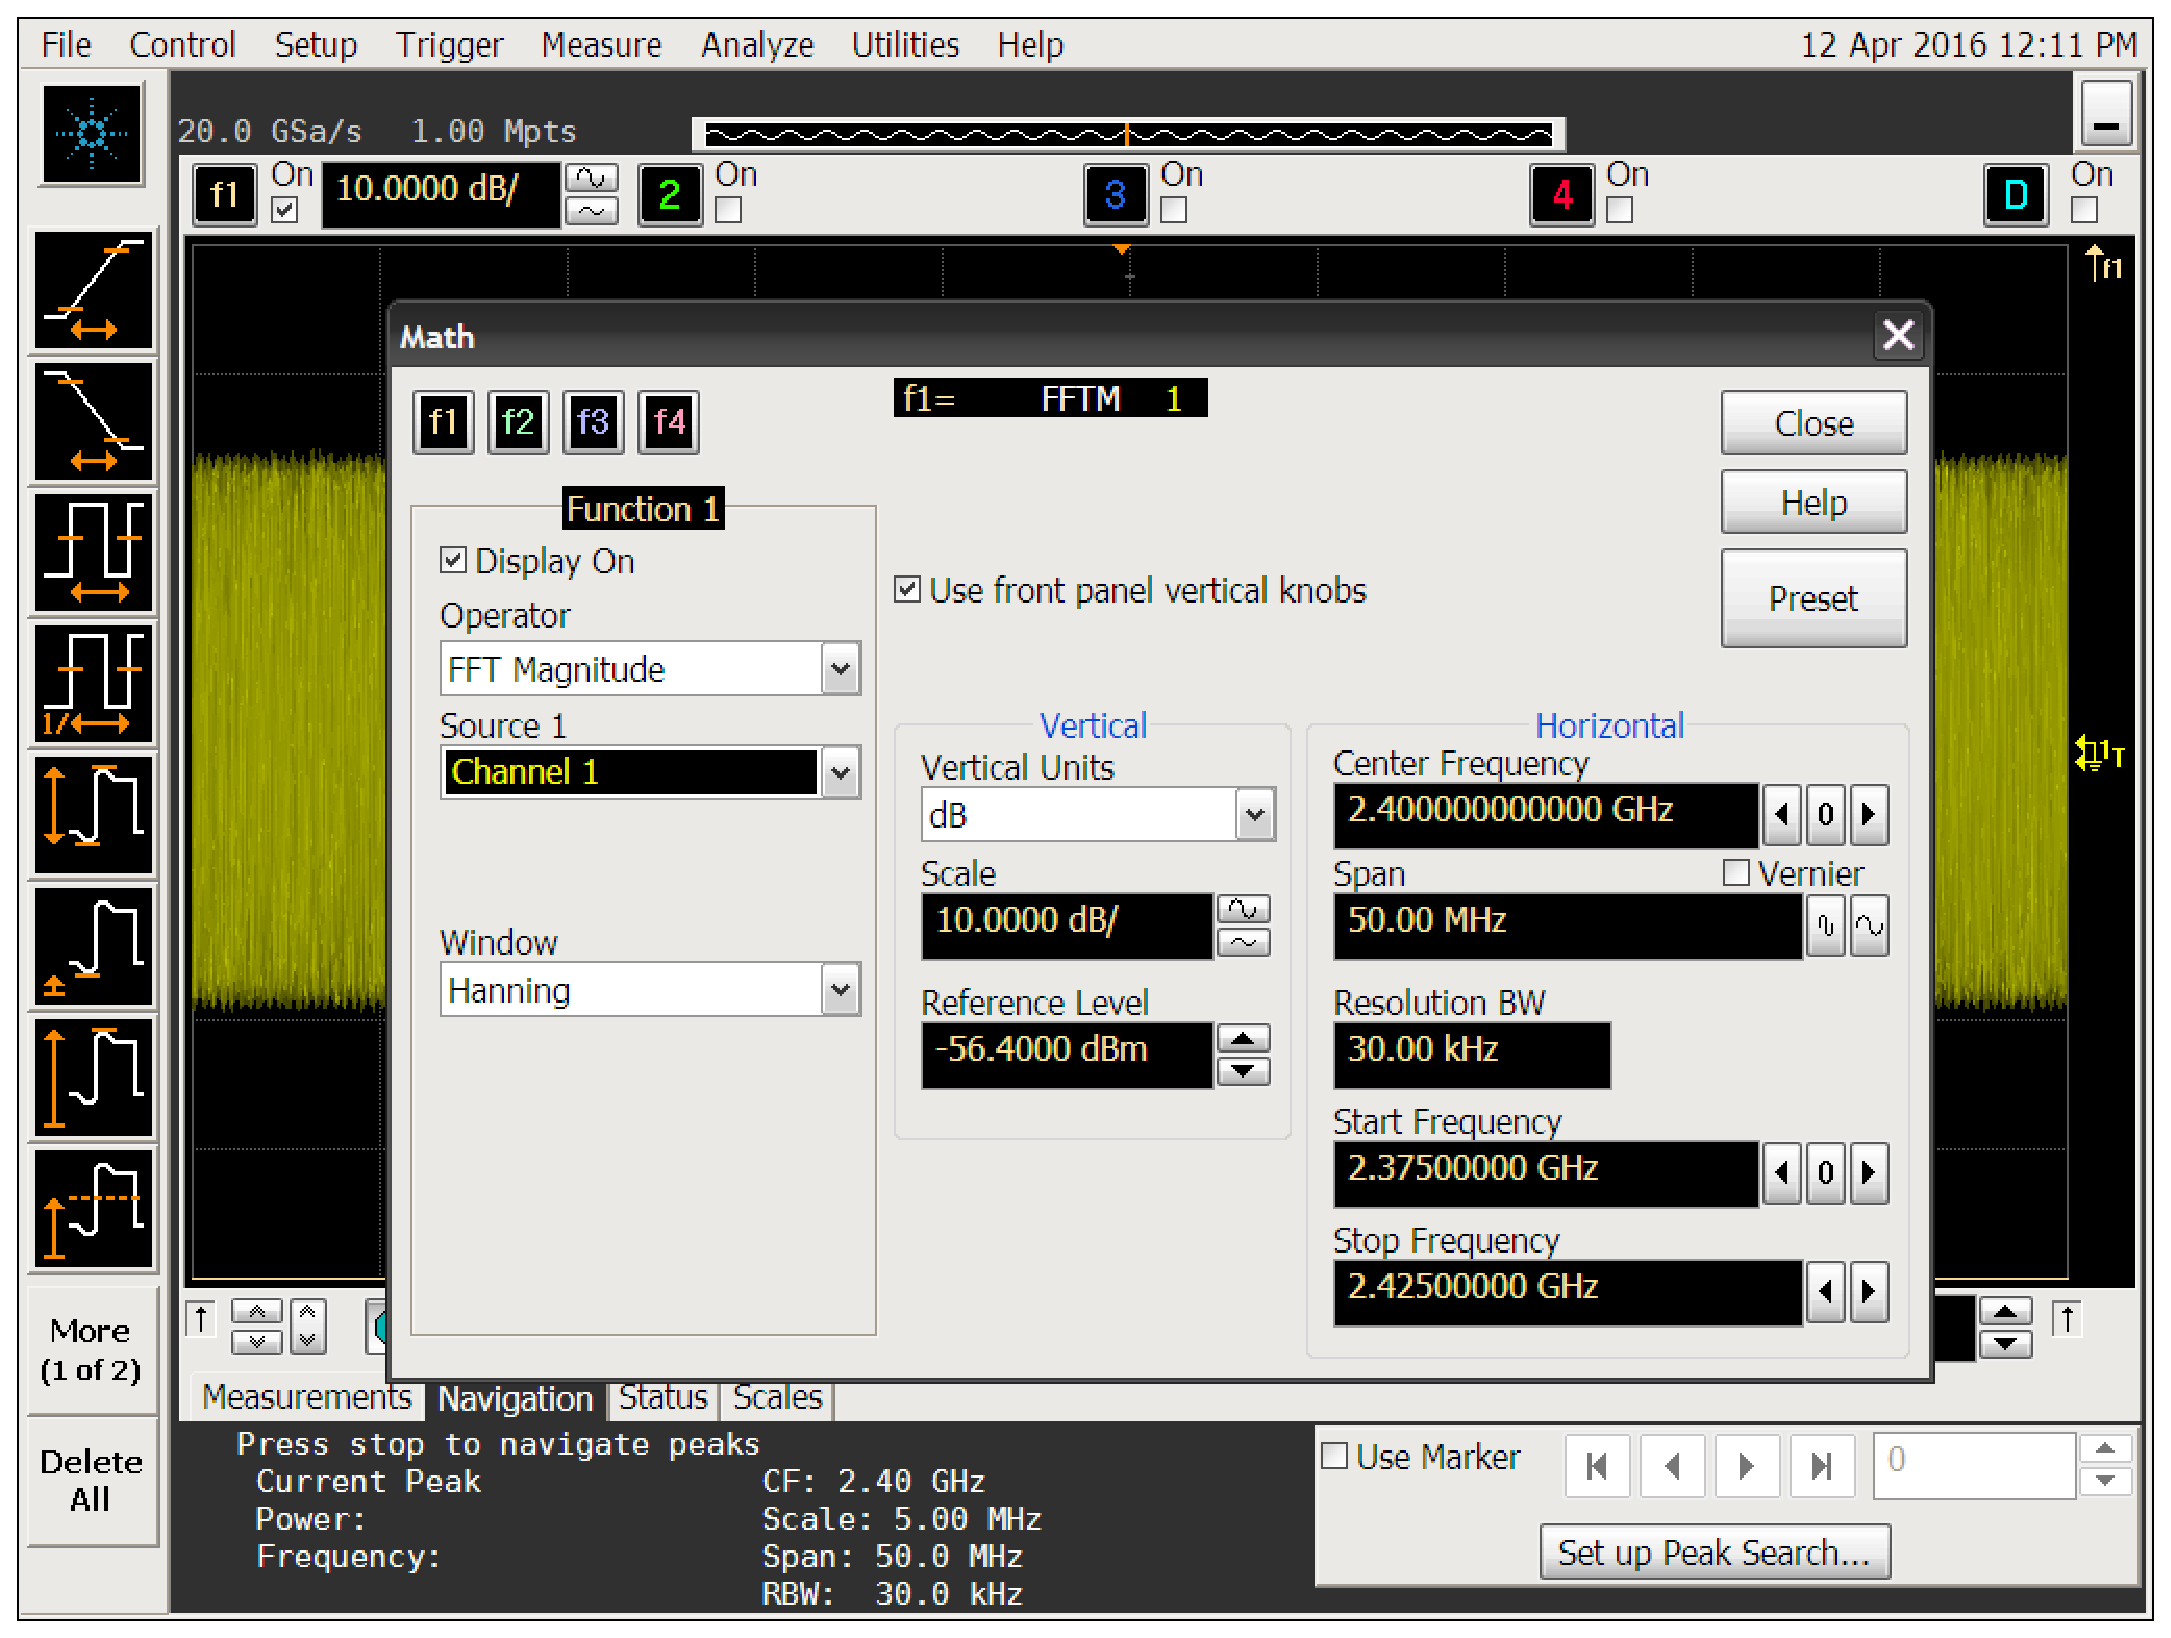
\includegraphics[width=0.85\textwidth]{./figures/oscill_fftcf}
    \caption{ FFT Configuration Parameters
    \label{fig:oscillfftcf}}
\end{figure}

%wave + fft
\begin{figure}[htbp]
    \centering
    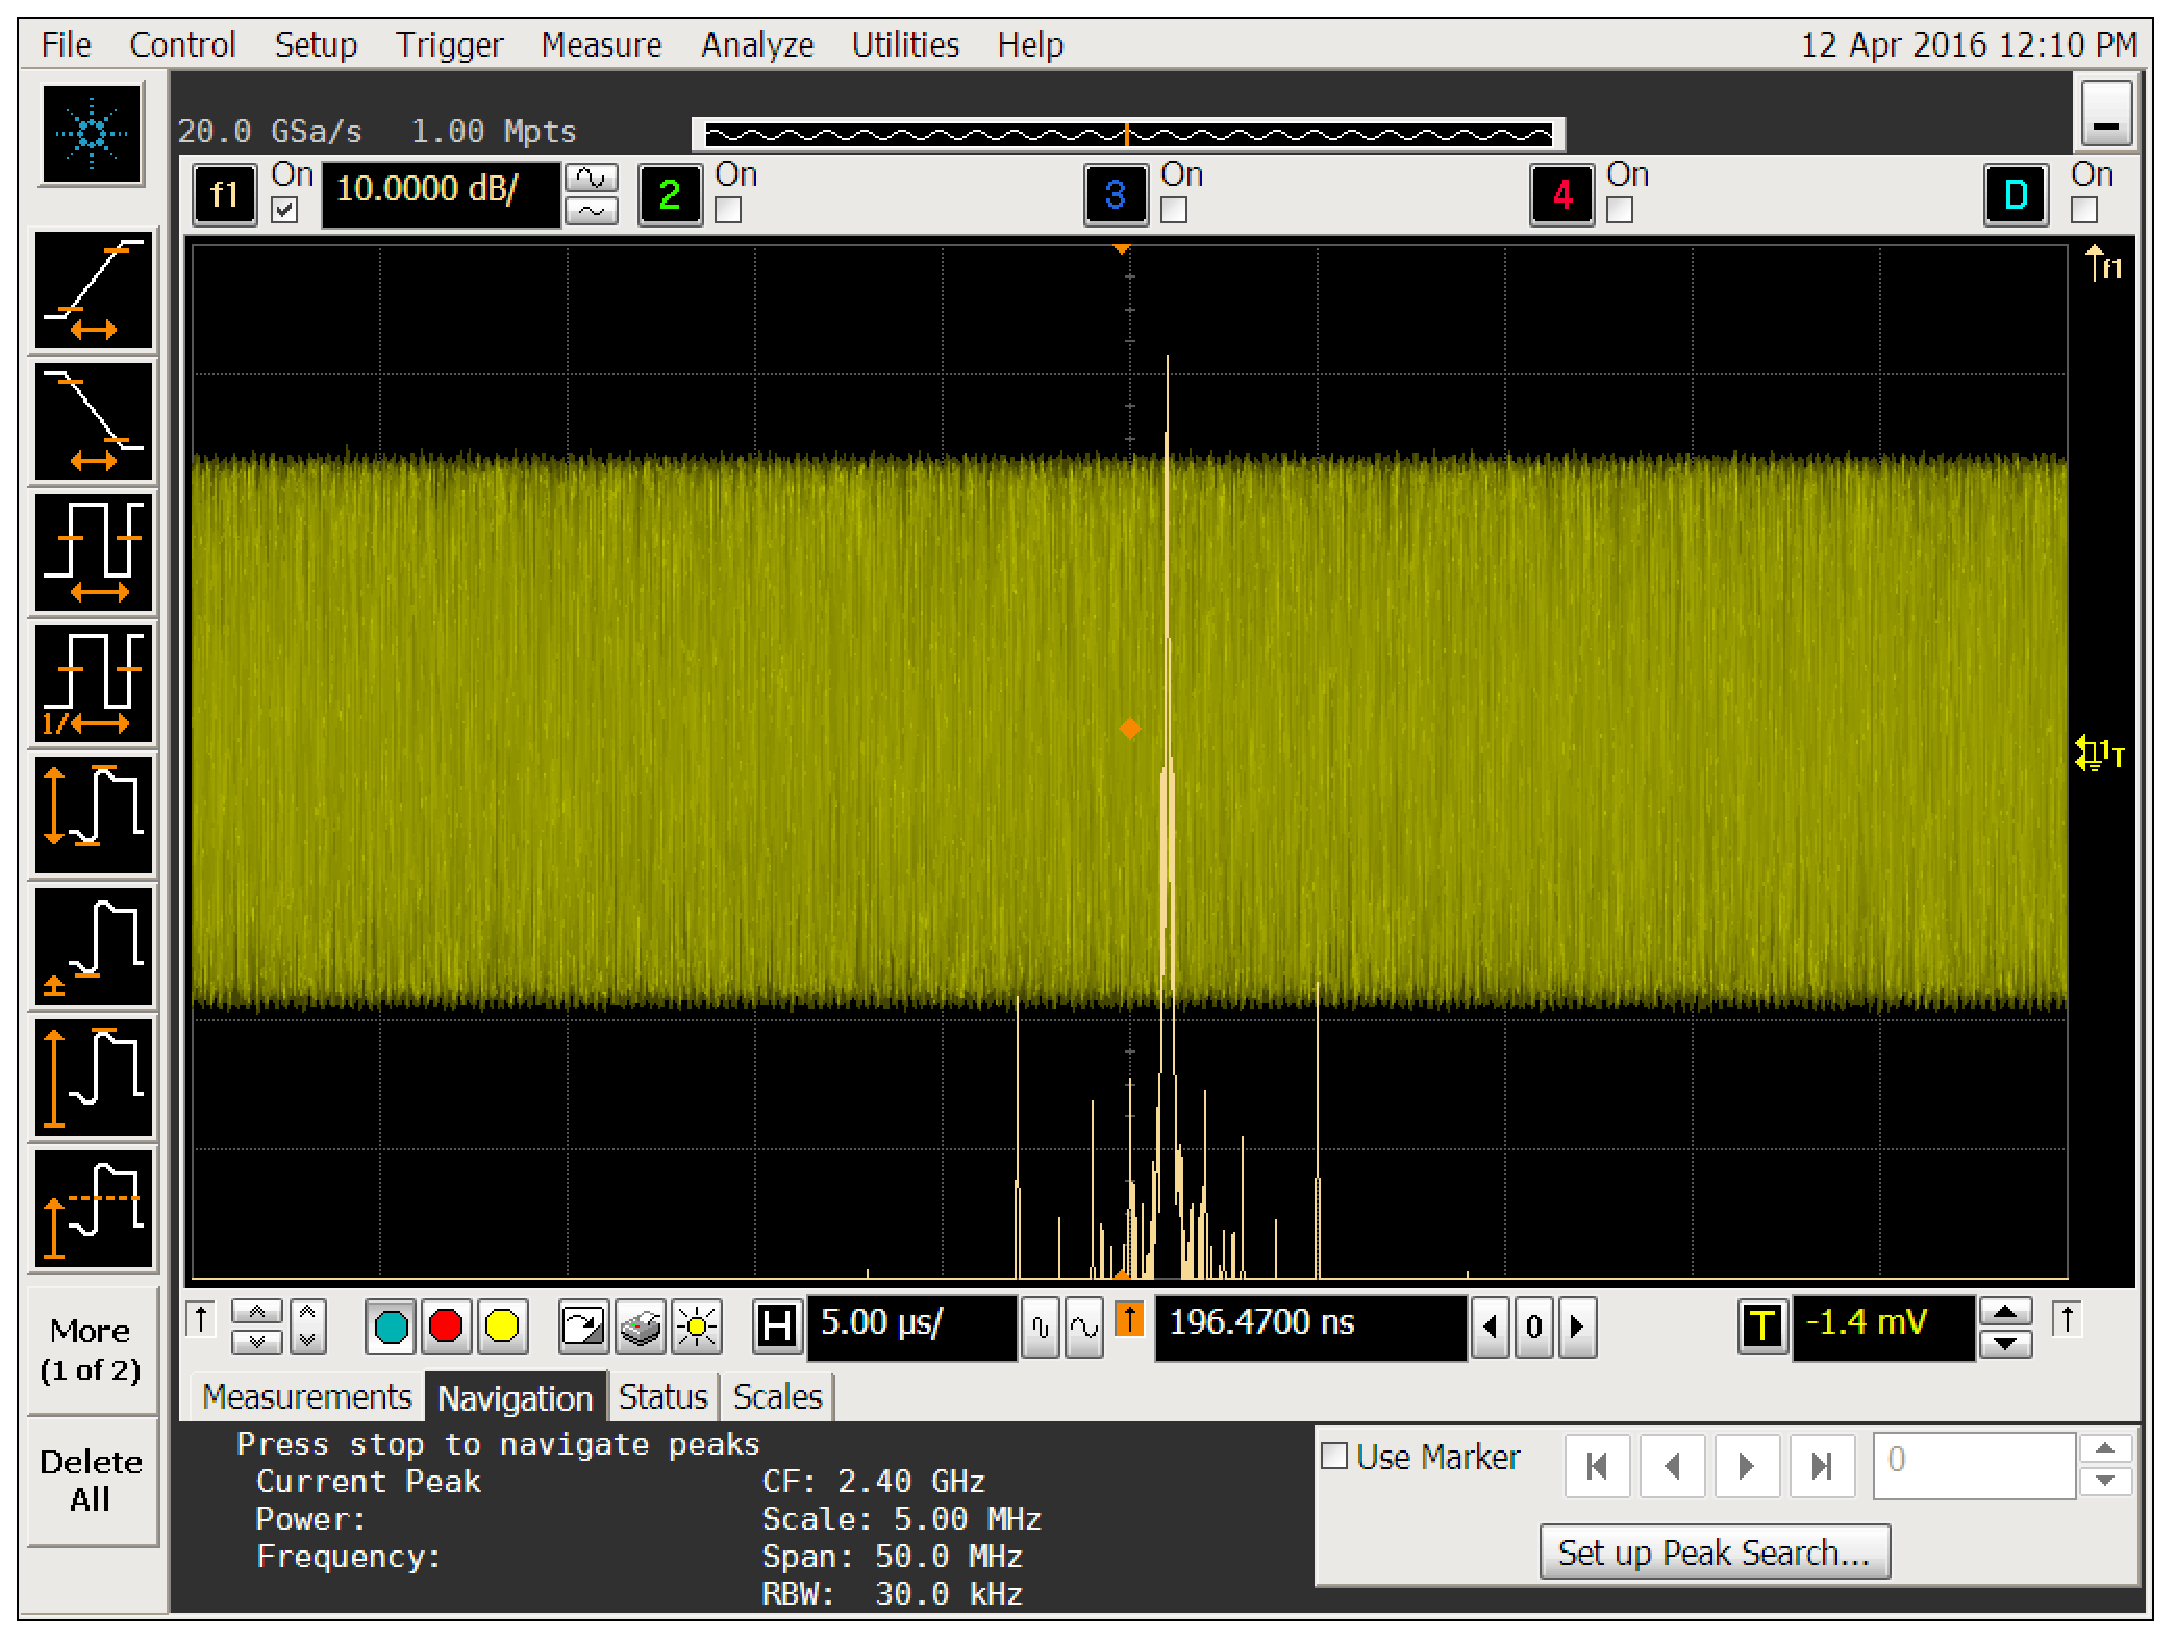
\includegraphics[width=0.85\textwidth]{./figures/oscill_fft}
    \caption{ FFT and Carrier Waveform
    \label{fig:oscillfft}}
\end{figure}

\vfill
\clearpage

\section{Simulation}

An important step in HDL development is the logic simulation of the circuit,
through this simulation it is possible to watch every port and be able to
understand the block behavior, thus correcting any problem or misbehavior.

\subsection{Transmit (DAC) Interface Simulation}

The simulation of the transmit interface, which interfaces the FPGA with DAC was
made in three steps, since the interface is composed by two blocks, there was
the need to simulate each block separately and after this simulate both blocks
connected and working together, in the figures \ref{fig:simdacdma},
\ref{fig:simdac} and \ref{fig:simtxif} it is possible to see the simulation
results and wave diagrams of the three steps.

In the figure \ref{fig:simdacdma} it is possible to watch the behavior of the
\textit{dac-dmaIterface} block where the signal \textit{sig\_dma\_data} is fed to
the block, and the signals \textit{ sig\_axis\_axc0\_itdata, sig\_axis\_axc0\_qtdata,
sig\_axis\_axc1\_itdata and sig\_axis\_axc1\_qtdata} are the \textit{IQ data} being
fed to both to the \textit{dacInterface} block.

\begin{figure}[htbp]
    \centering
    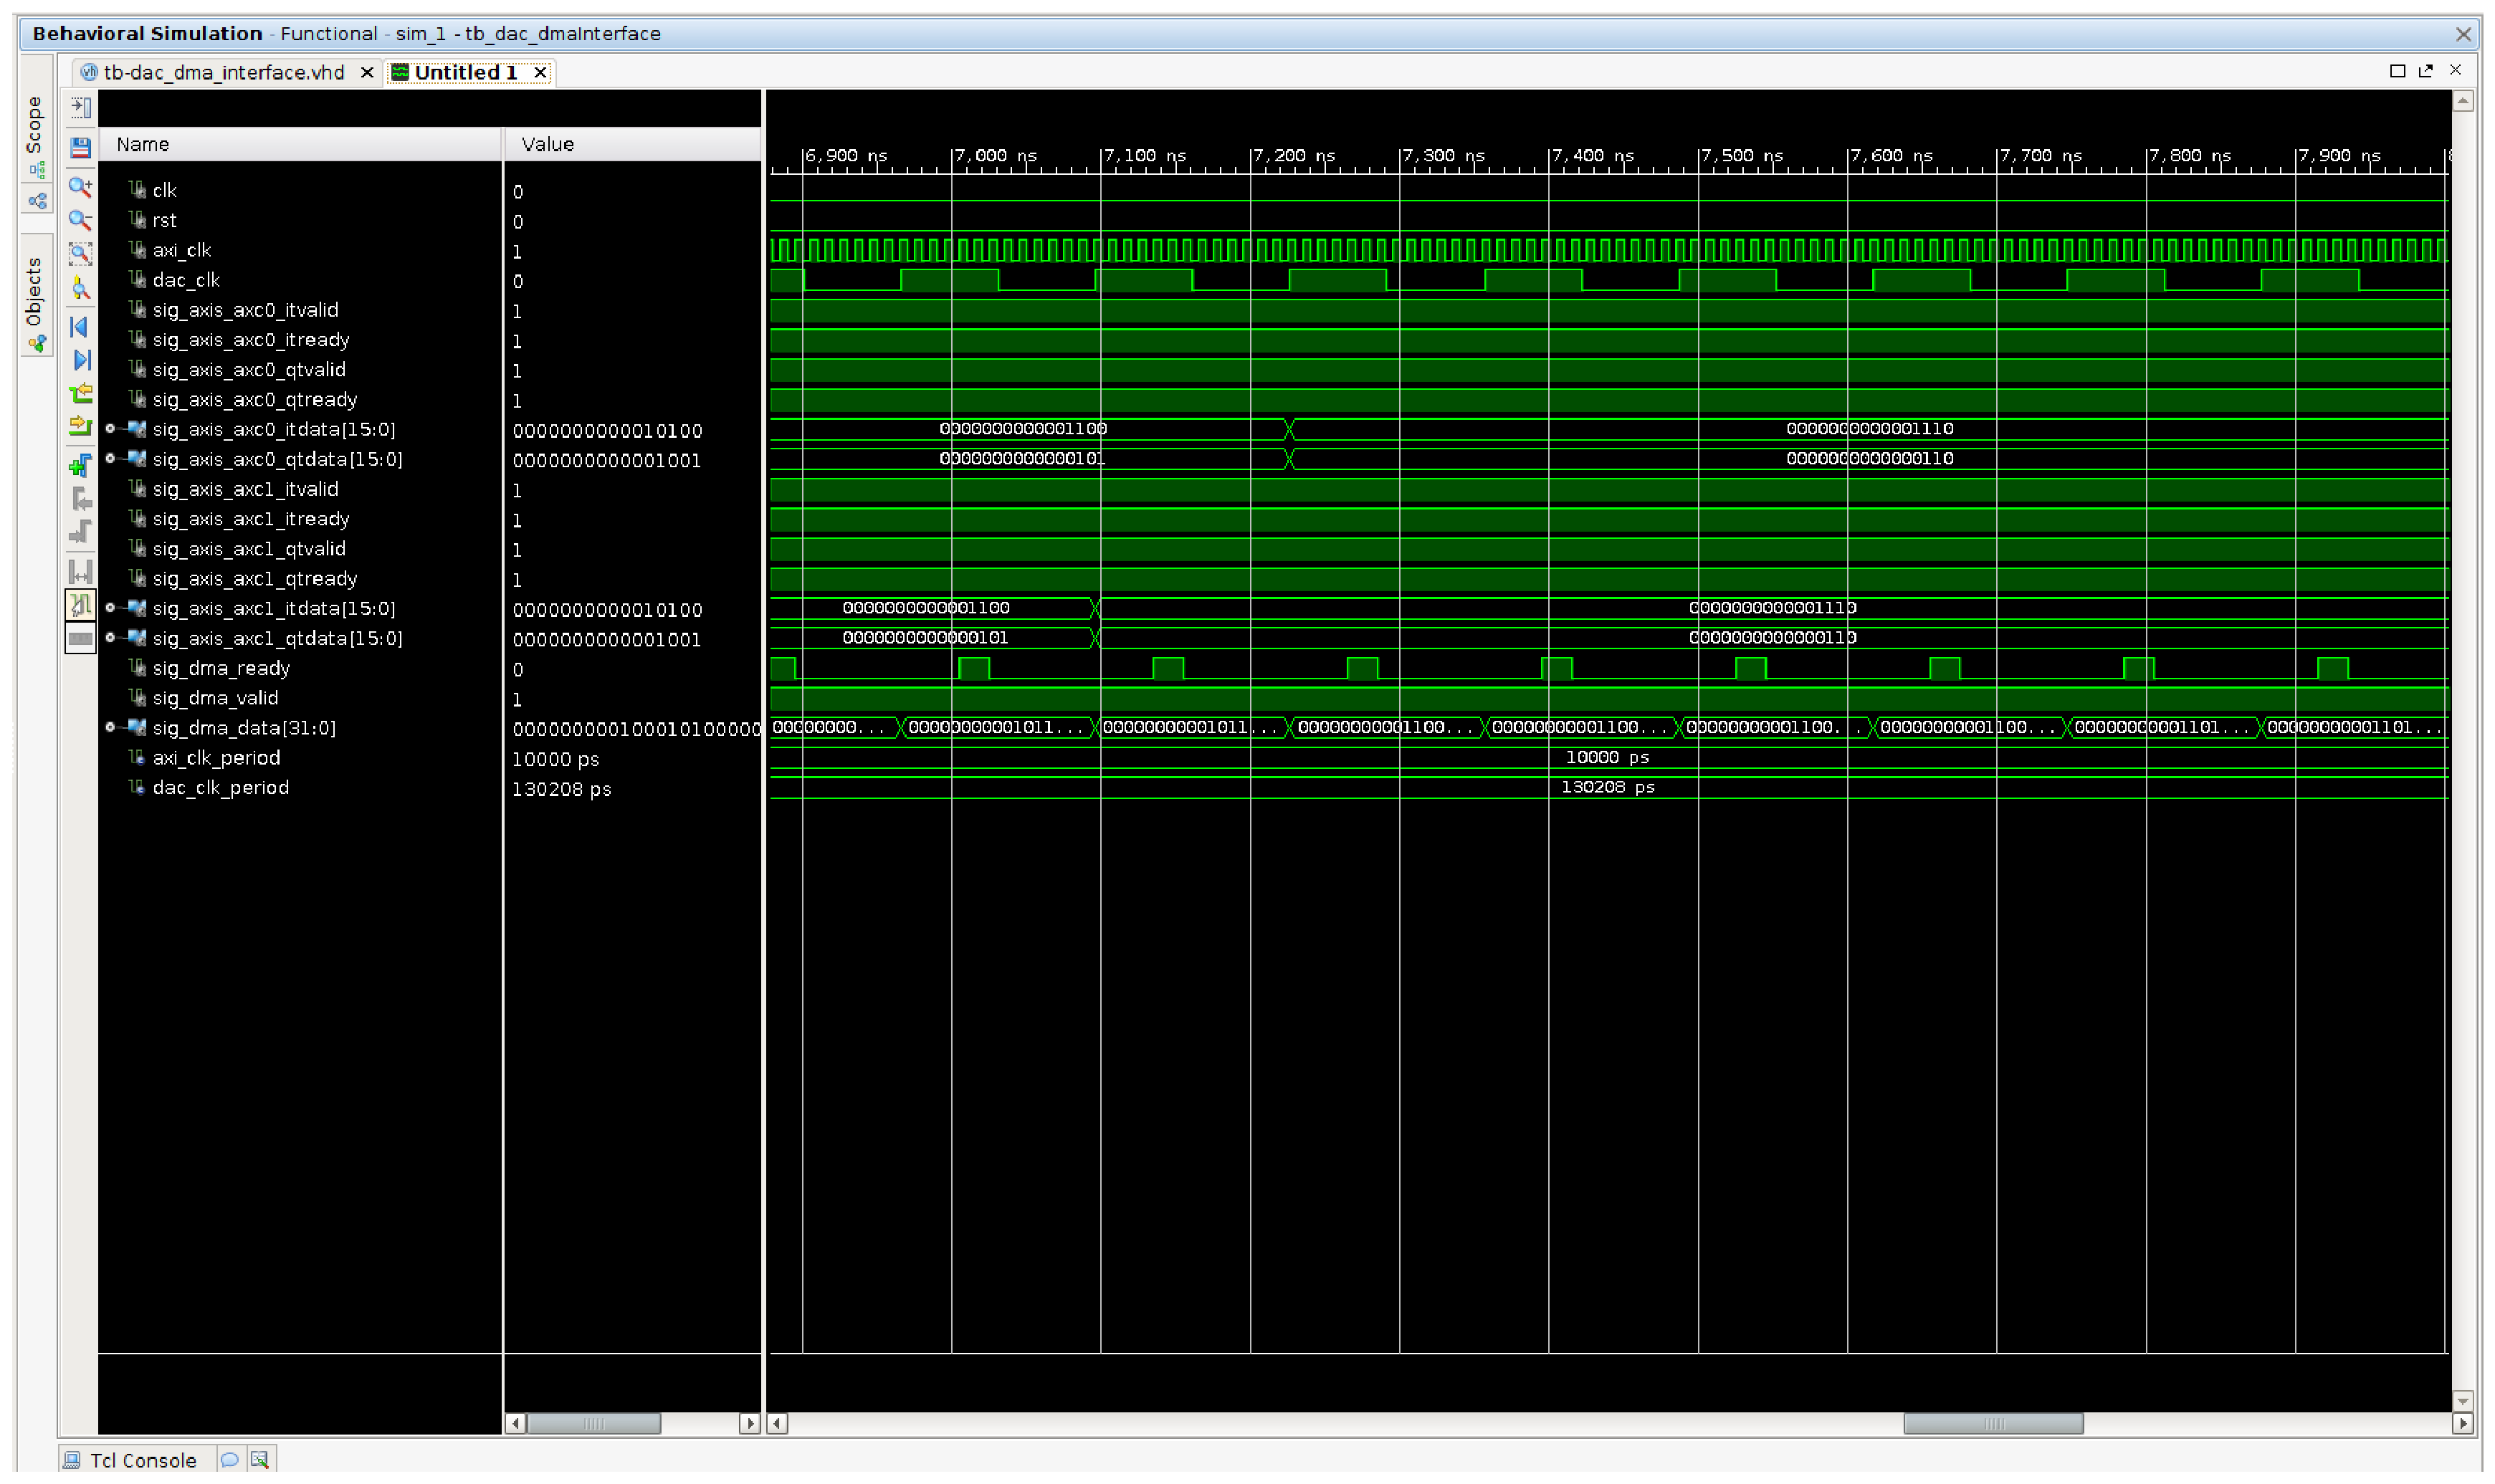
\includegraphics[width=0.95\textwidth]{./figures/dac_dmaInterface}
    \caption{ Step 1: DAC-DMA Interface Block Simulation
    \label{fig:simdacdma}}
\end{figure}

 In the figure \ref{fig:simdac} the \textit{dacInterface} is simulated and again
 it is possible to watch teh signals \textit{sig\_axis\_axc0\_itdata,
 sig\_axis\_axc0\_qtdata, sig\_axis\_axc1\_itdata and sig\_axis\_axc1\_qtdata} being fed
 to the block and the outputs \textit{sig\_dac\_i0data, sig\_dac\_q0data,
 sig\_dac\_i1data and sig\_dac\_q1data}, teh point in both \textit{dac-dmaIterface}
 and \textit{dacInterface} is to watch ghanges in outputs accompanying
 \textit{ready and valid} signals whcih are used as a way of controlling reading
 speed from the \textit{DMA}, in such scheme, the \textit{DMA} assets
 \textit{valid} whenever is can send data, however it only send teh data when
 fed by a ready signal, meaning that the reading block can read the \textit{DMA}
 data.

\begin{figure}[htbp]
    \centering
    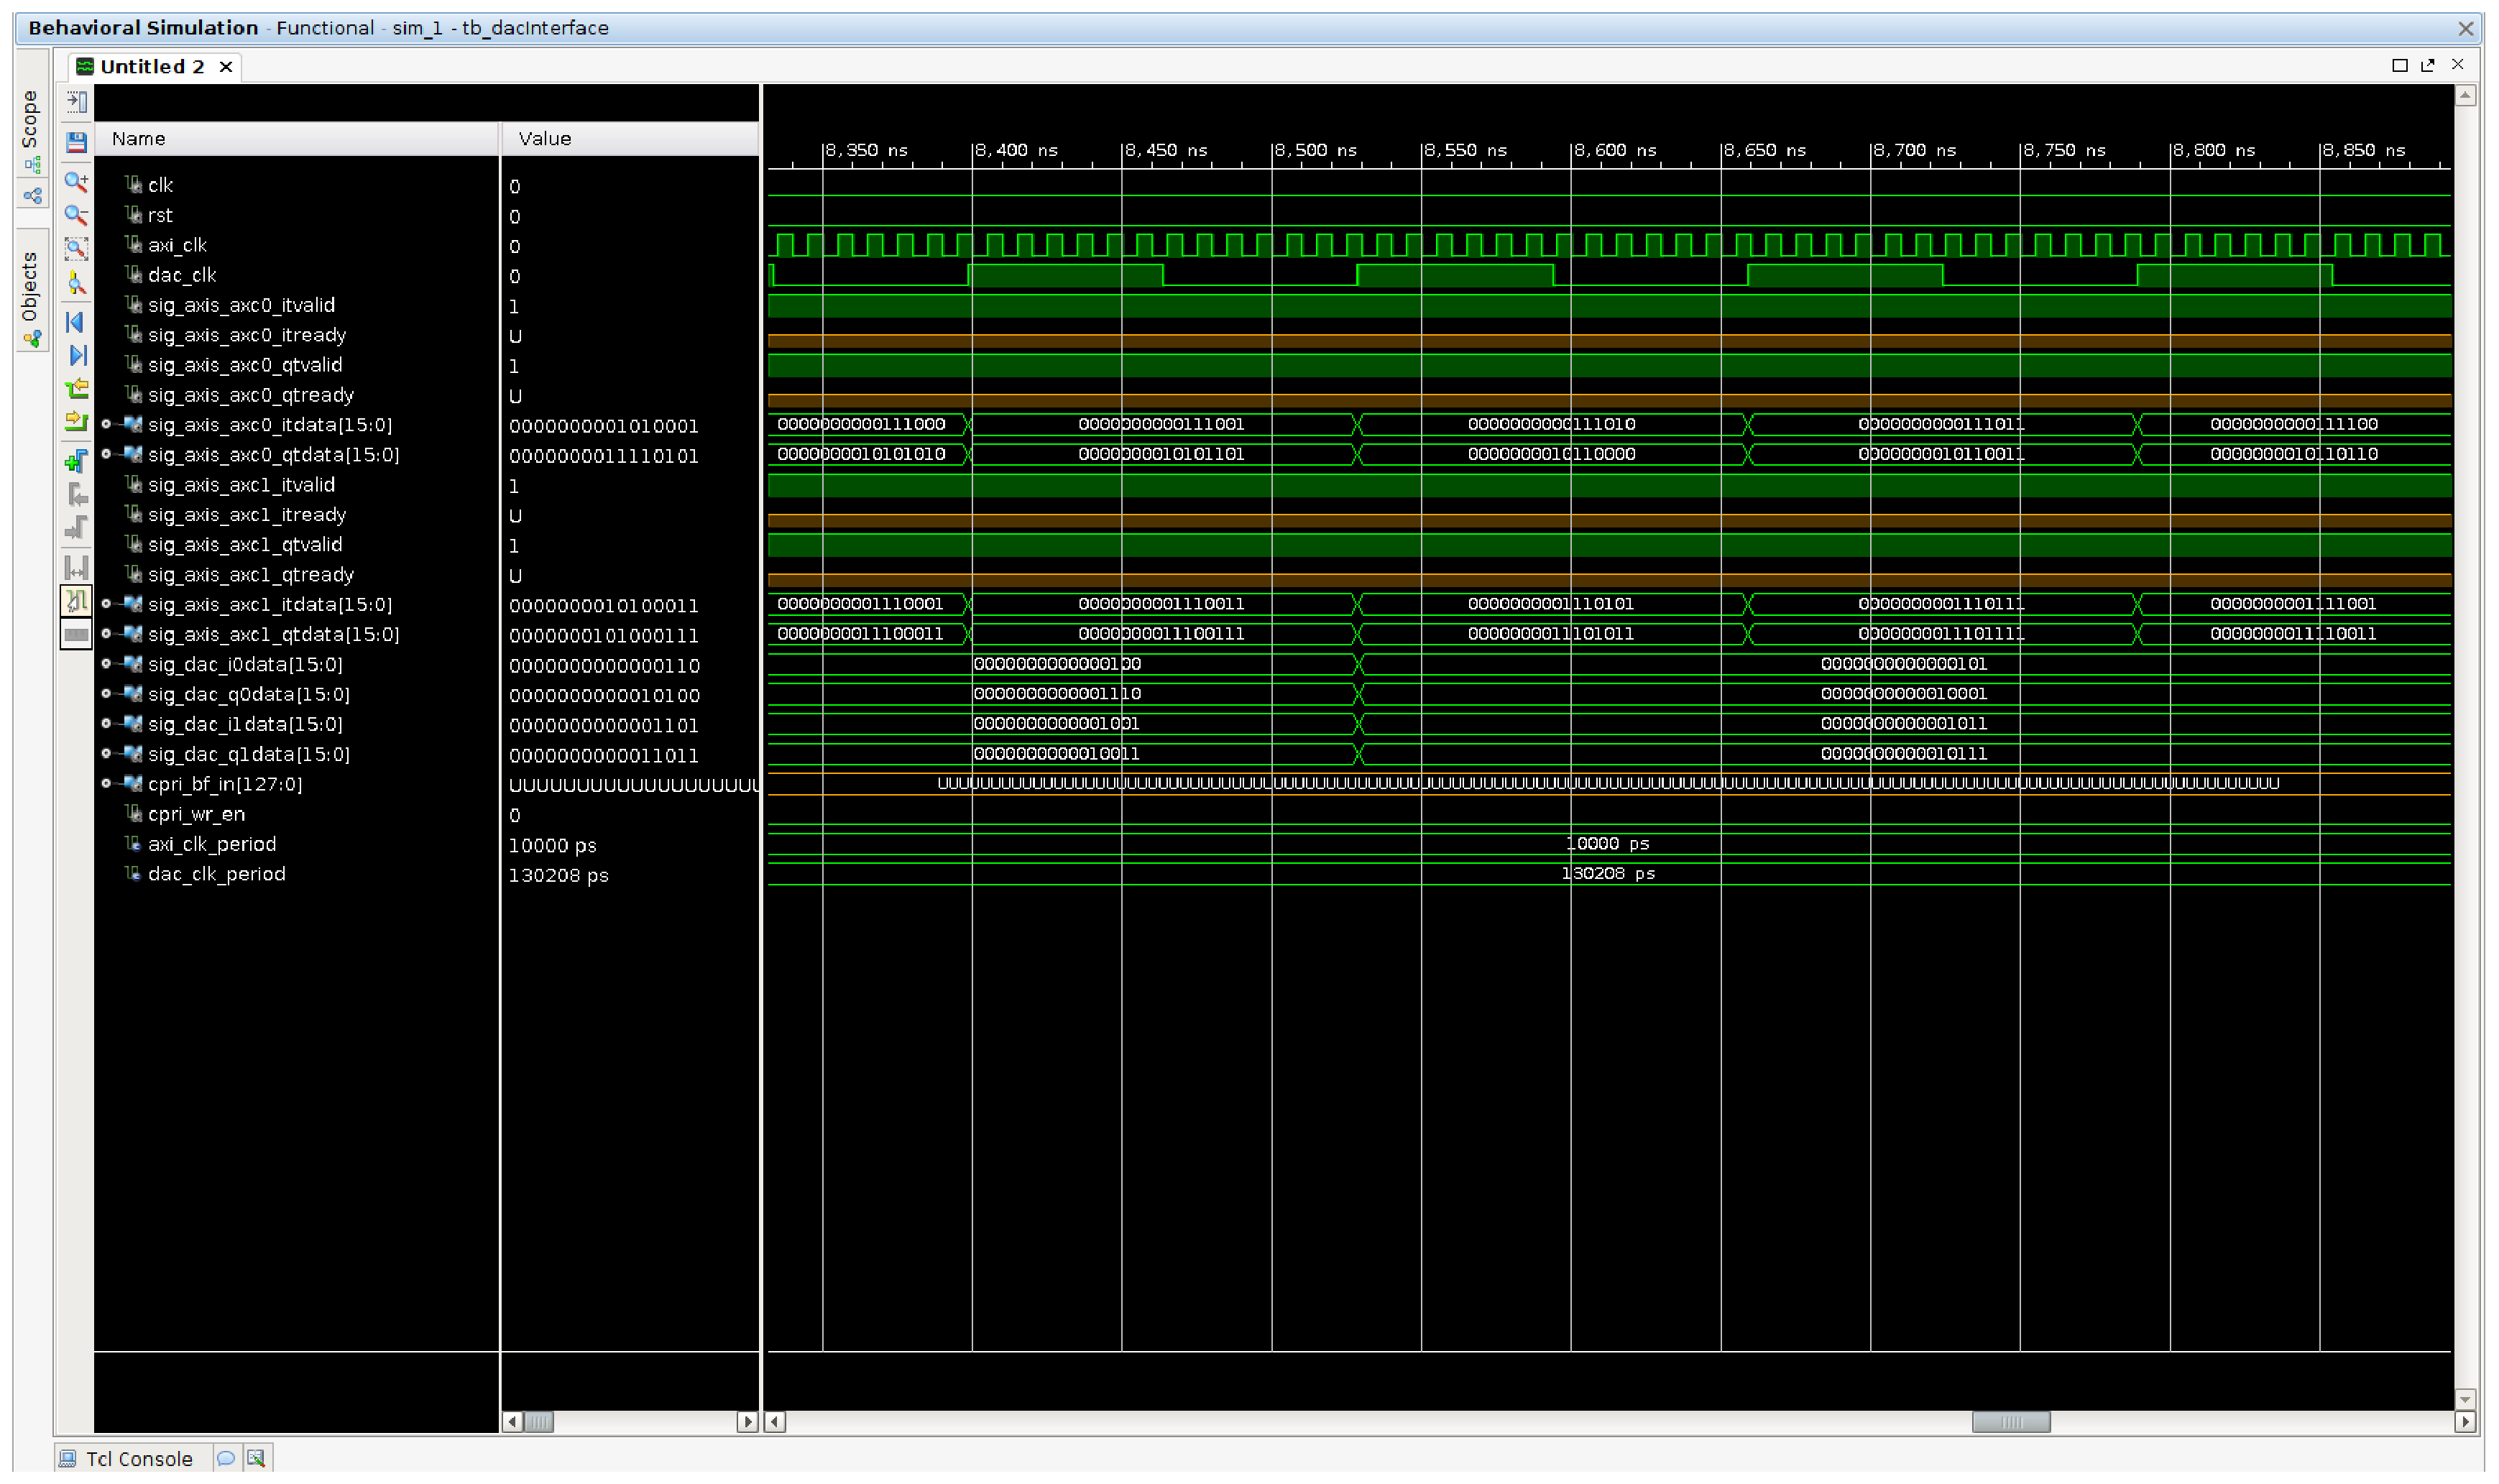
\includegraphics[width=0.95\textwidth]{./figures/dacInterface}
    \caption{ Step 2: DAC Interface Block Simulation
    \label{fig:simdac}}
\end{figure}

In the final simulation of the transmitting interface the whole transmit chain
blocks were simulated toghether and then is is possible to understand the
behavior of the whole transmit interface block. In the figure \ref{fig:simtxif}
it is possible to watch the \textit{DMA} data in the signal in
\textit{dac-dmaIterface} and the outputs which woul fedd the \textit{AD9361}
two \textit{DACs} in the signals \textit{sig\_dac\_i0data, sig\_dac\_q0data,
sig\_dac\_i1data and sig\_dac\_q1data}, again the important thing in the simulation
is to watch for the data change and the  \textit{ready and valid} changes.
Another interesting thing to observ is the two clock variables \textit{axi\_clk}
and \textit{dac\_clk} which represent both axi system clock $ 100 MHz$ and the
dac clock $40 MHz$, this difference justifies the use of such interface.


\begin{figure}[htbp]
    \centering
    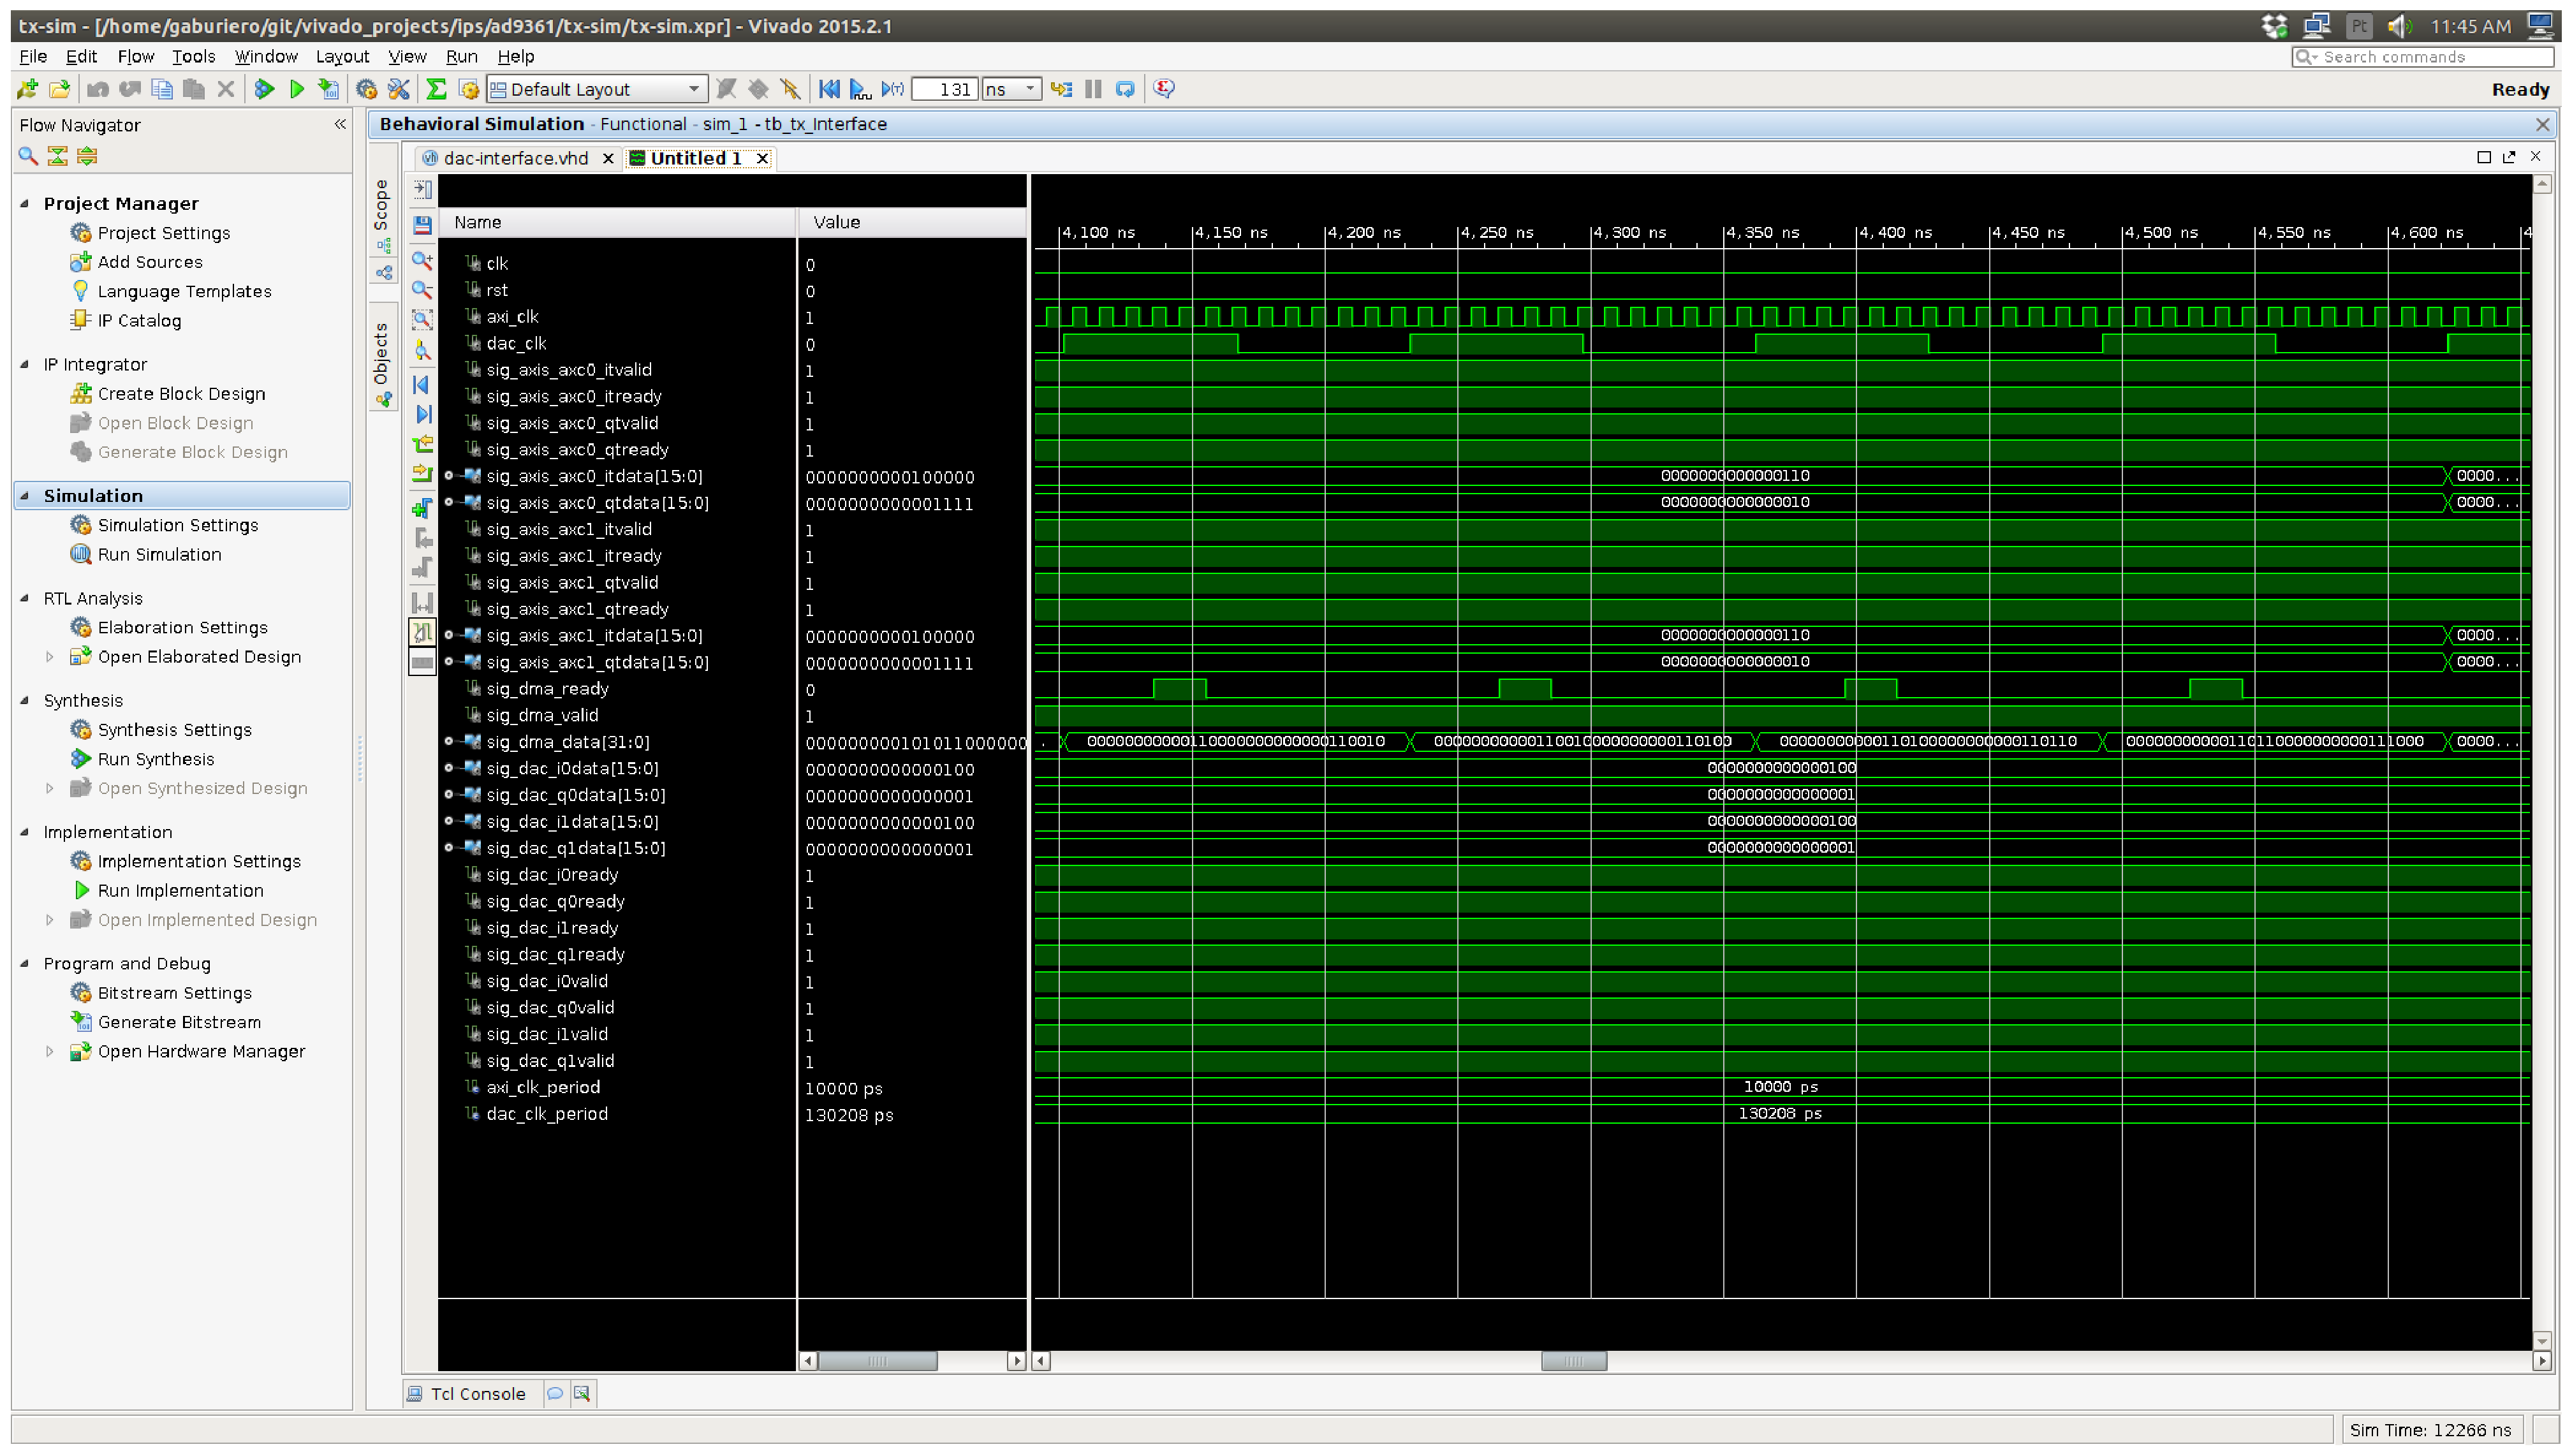
\includegraphics[width=0.95\textwidth]{./figures/txInterface}
    \caption{ Step 3: Transmitting Interface Block Simulation
    \label{fig:simtxif}}
\end{figure}

\subsection{Receive (ADC) Interface Simulation}

As stated before on chapter \ref{chap:implementation} in the section \ref{impl:setup},
the DAC interface is simple beacause the data input is already limited by the DAC
clock, so there is no need to make a bottleneck like in the DAC interface.

 In the figure \ref{fig:simdac} it is possible to see the output and wave
diagram in the simulation window. Since the \textit{adcInterface} is much more
simpler, because the data input is already limited by the \textit{AD9361}
clock, in the signals \textit{sig\_rx\_i0\_data, sig\_rx\_q0\_data,
sig\_rx\_i1\_data, sig\_rx\_q1\_data} there is the outputs from both
\textit{DACs} and \textit{dout} is the data that will be fed to the
\textit{DMA}.\\

\begin{figure}[htbp]
    \centering
    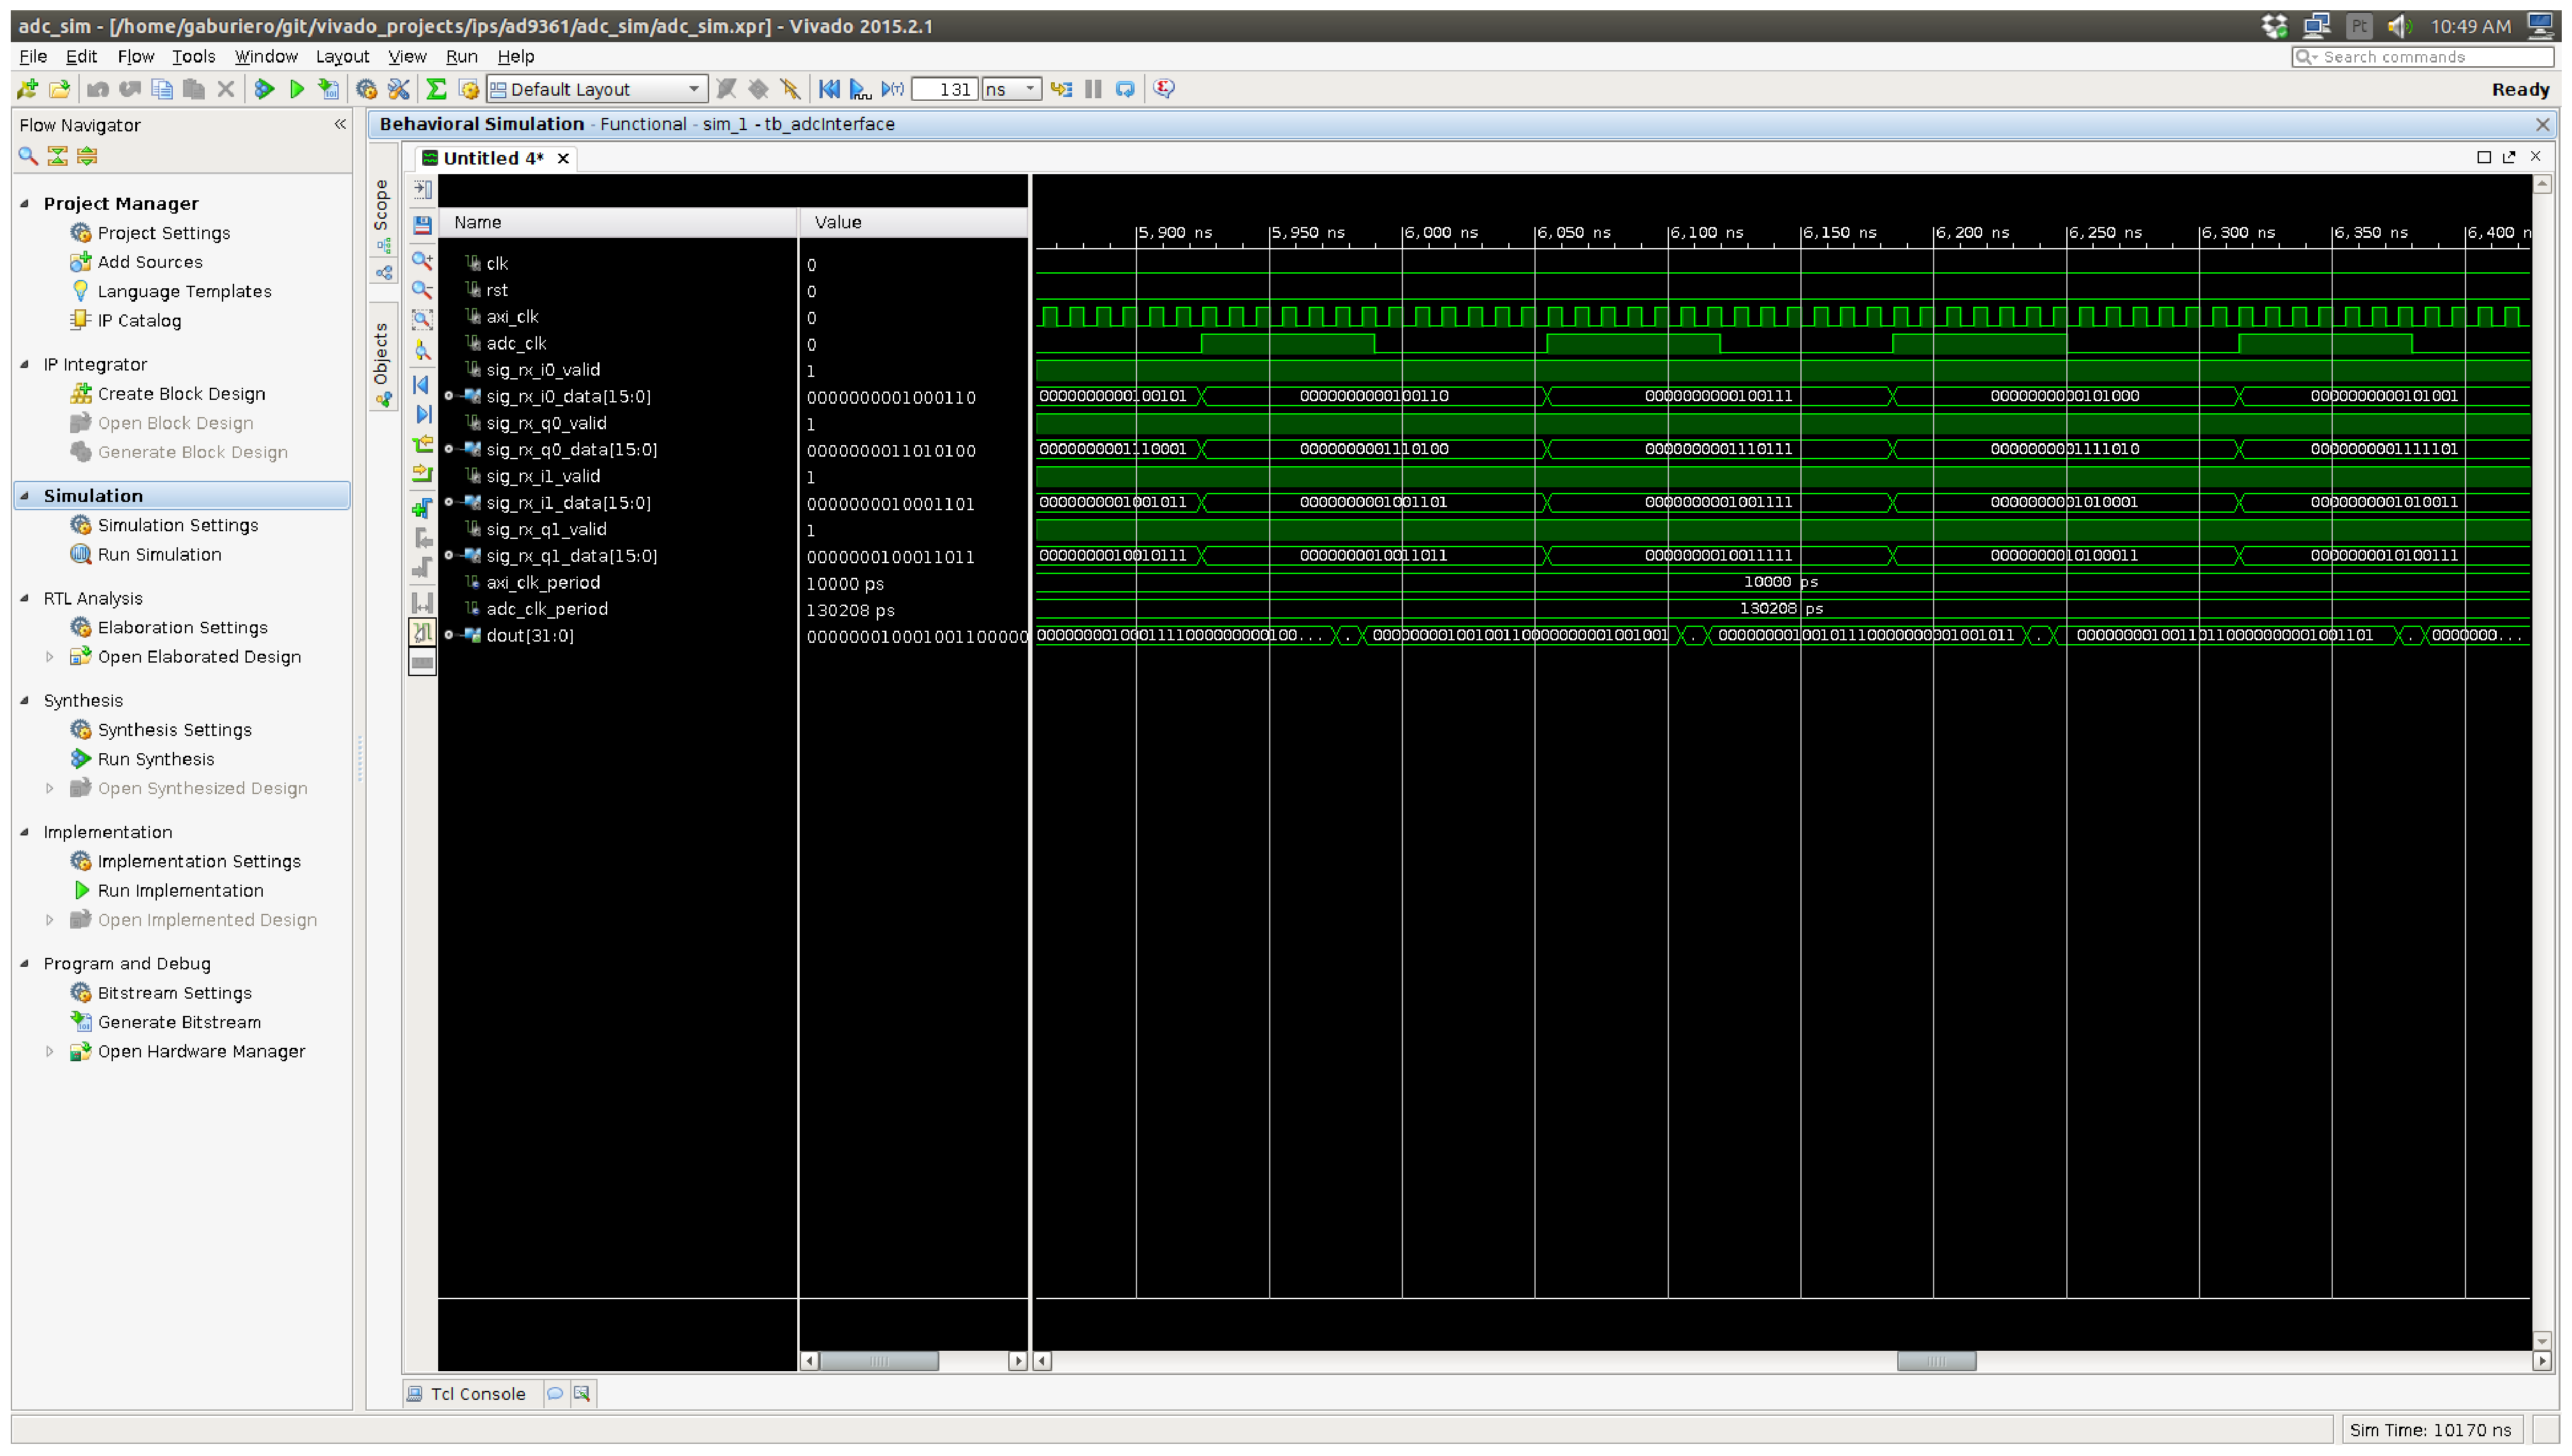
\includegraphics[width=0.95\textwidth]{./figures/adcInterface}
    \caption{ ADC Interface Block Simulation
    \label{fig:simadc}}
\end{figure}

\vfill
\clearpage

\section{Transmission Tests (DAC)}
\label{result:dac}

 The transmission tests aim to evaluate a Donwlink LTE transmission, it means
that the data is being transmitted from the BTS to the UE. In this trnasmission
test there were generated LTE samples in matlab, and these samples were loaded
in the memory by putting them in a header file, the as explained before, DMA
shall read them and the DAC shall make an analog output. In the figure
\ref{fig:dacsignals} there are the DAC control signals sent to the data
interface block in order to control the data flow, thus this control makes a
back-pressure in the DMA engine controlling if DMA reads or not data from
memory, thus the DMA Engine reading output can be seen in the figures
\ref{fig:dataflowdig} and \ref{fig:dataflowana}, digital and analog waveforms
respectively.\\

 It is possible to configure in the driver if the AD9361 ouputs or not a clock
in a special clock\_output pin, so in order to evaluate frequency and clock
quality, the figure \ref{fig:dacclk} shows the clock output from the AD9361 and
last but not least the figure \ref{fig:lte5m} show the output spectrum of the
LTE analog wave outputted from the FMComms2 board.

\begin{figure}[htbp]
    \centering
    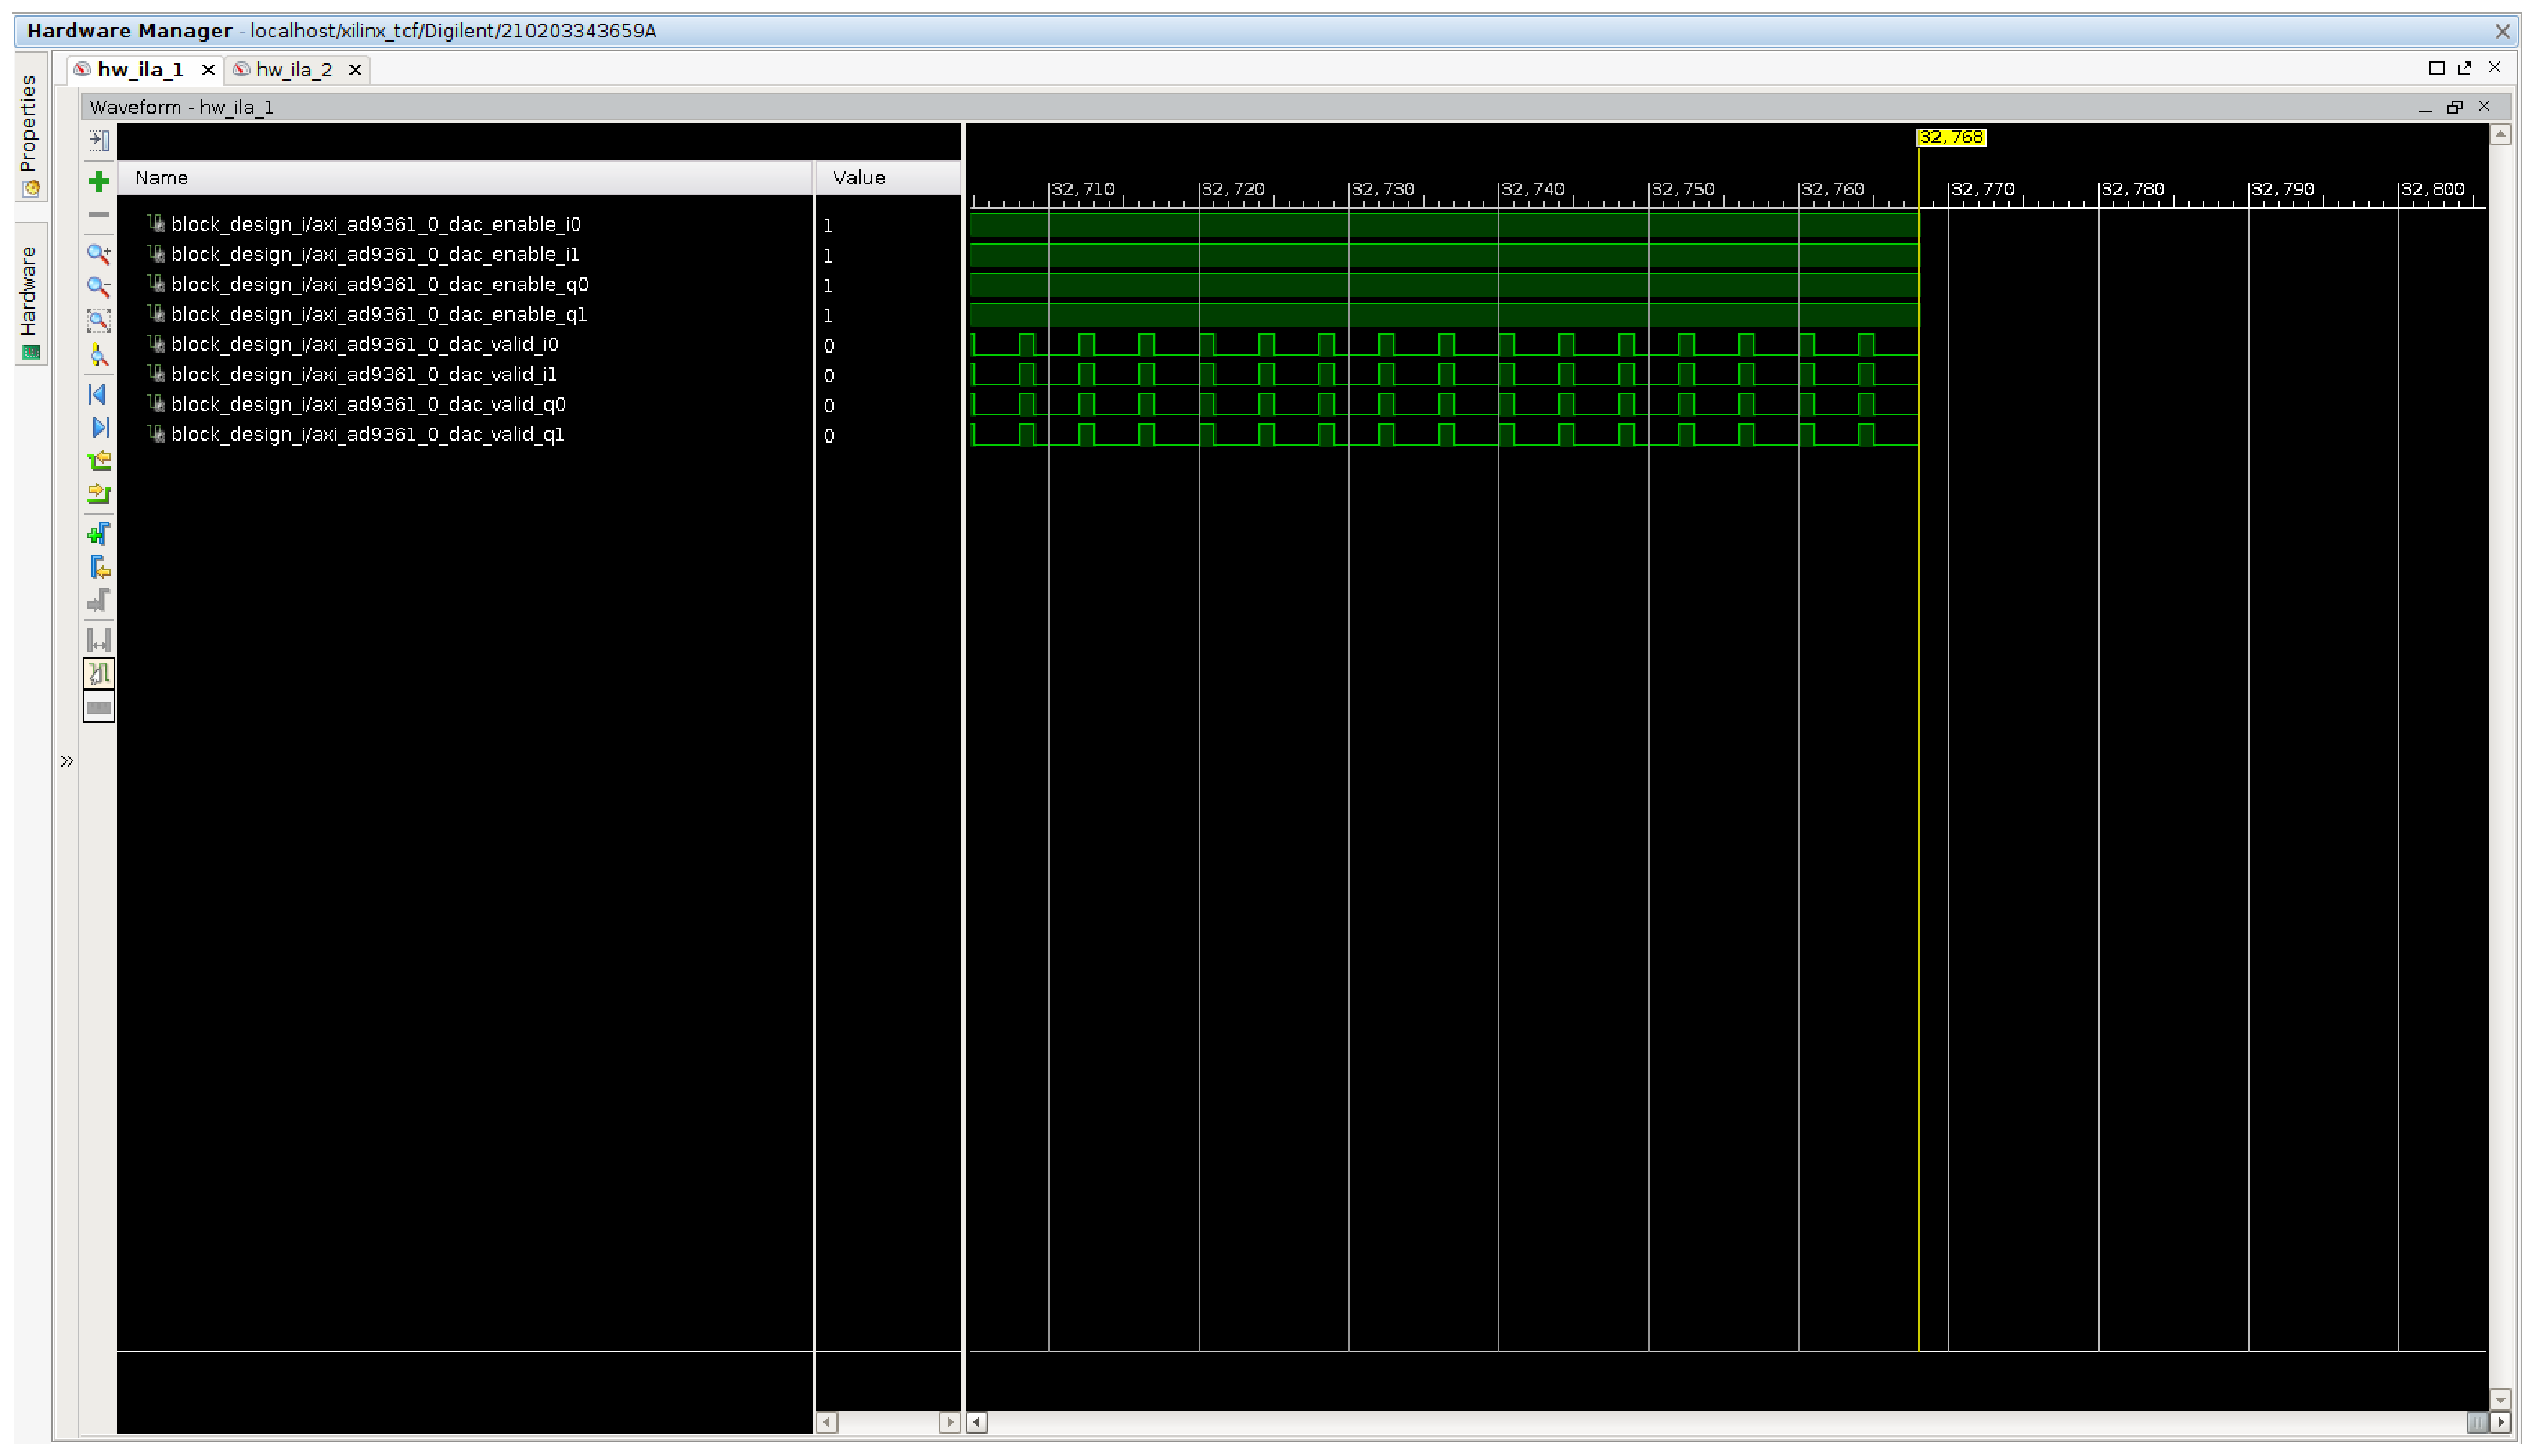
\includegraphics[width=0.85\textwidth]{./figures/dac_signals}
    \caption{ DAC signals controlling data reading
    \label{fig:dacsignals}}
\end{figure}

\begin{figure}[htbp]
    \centering
    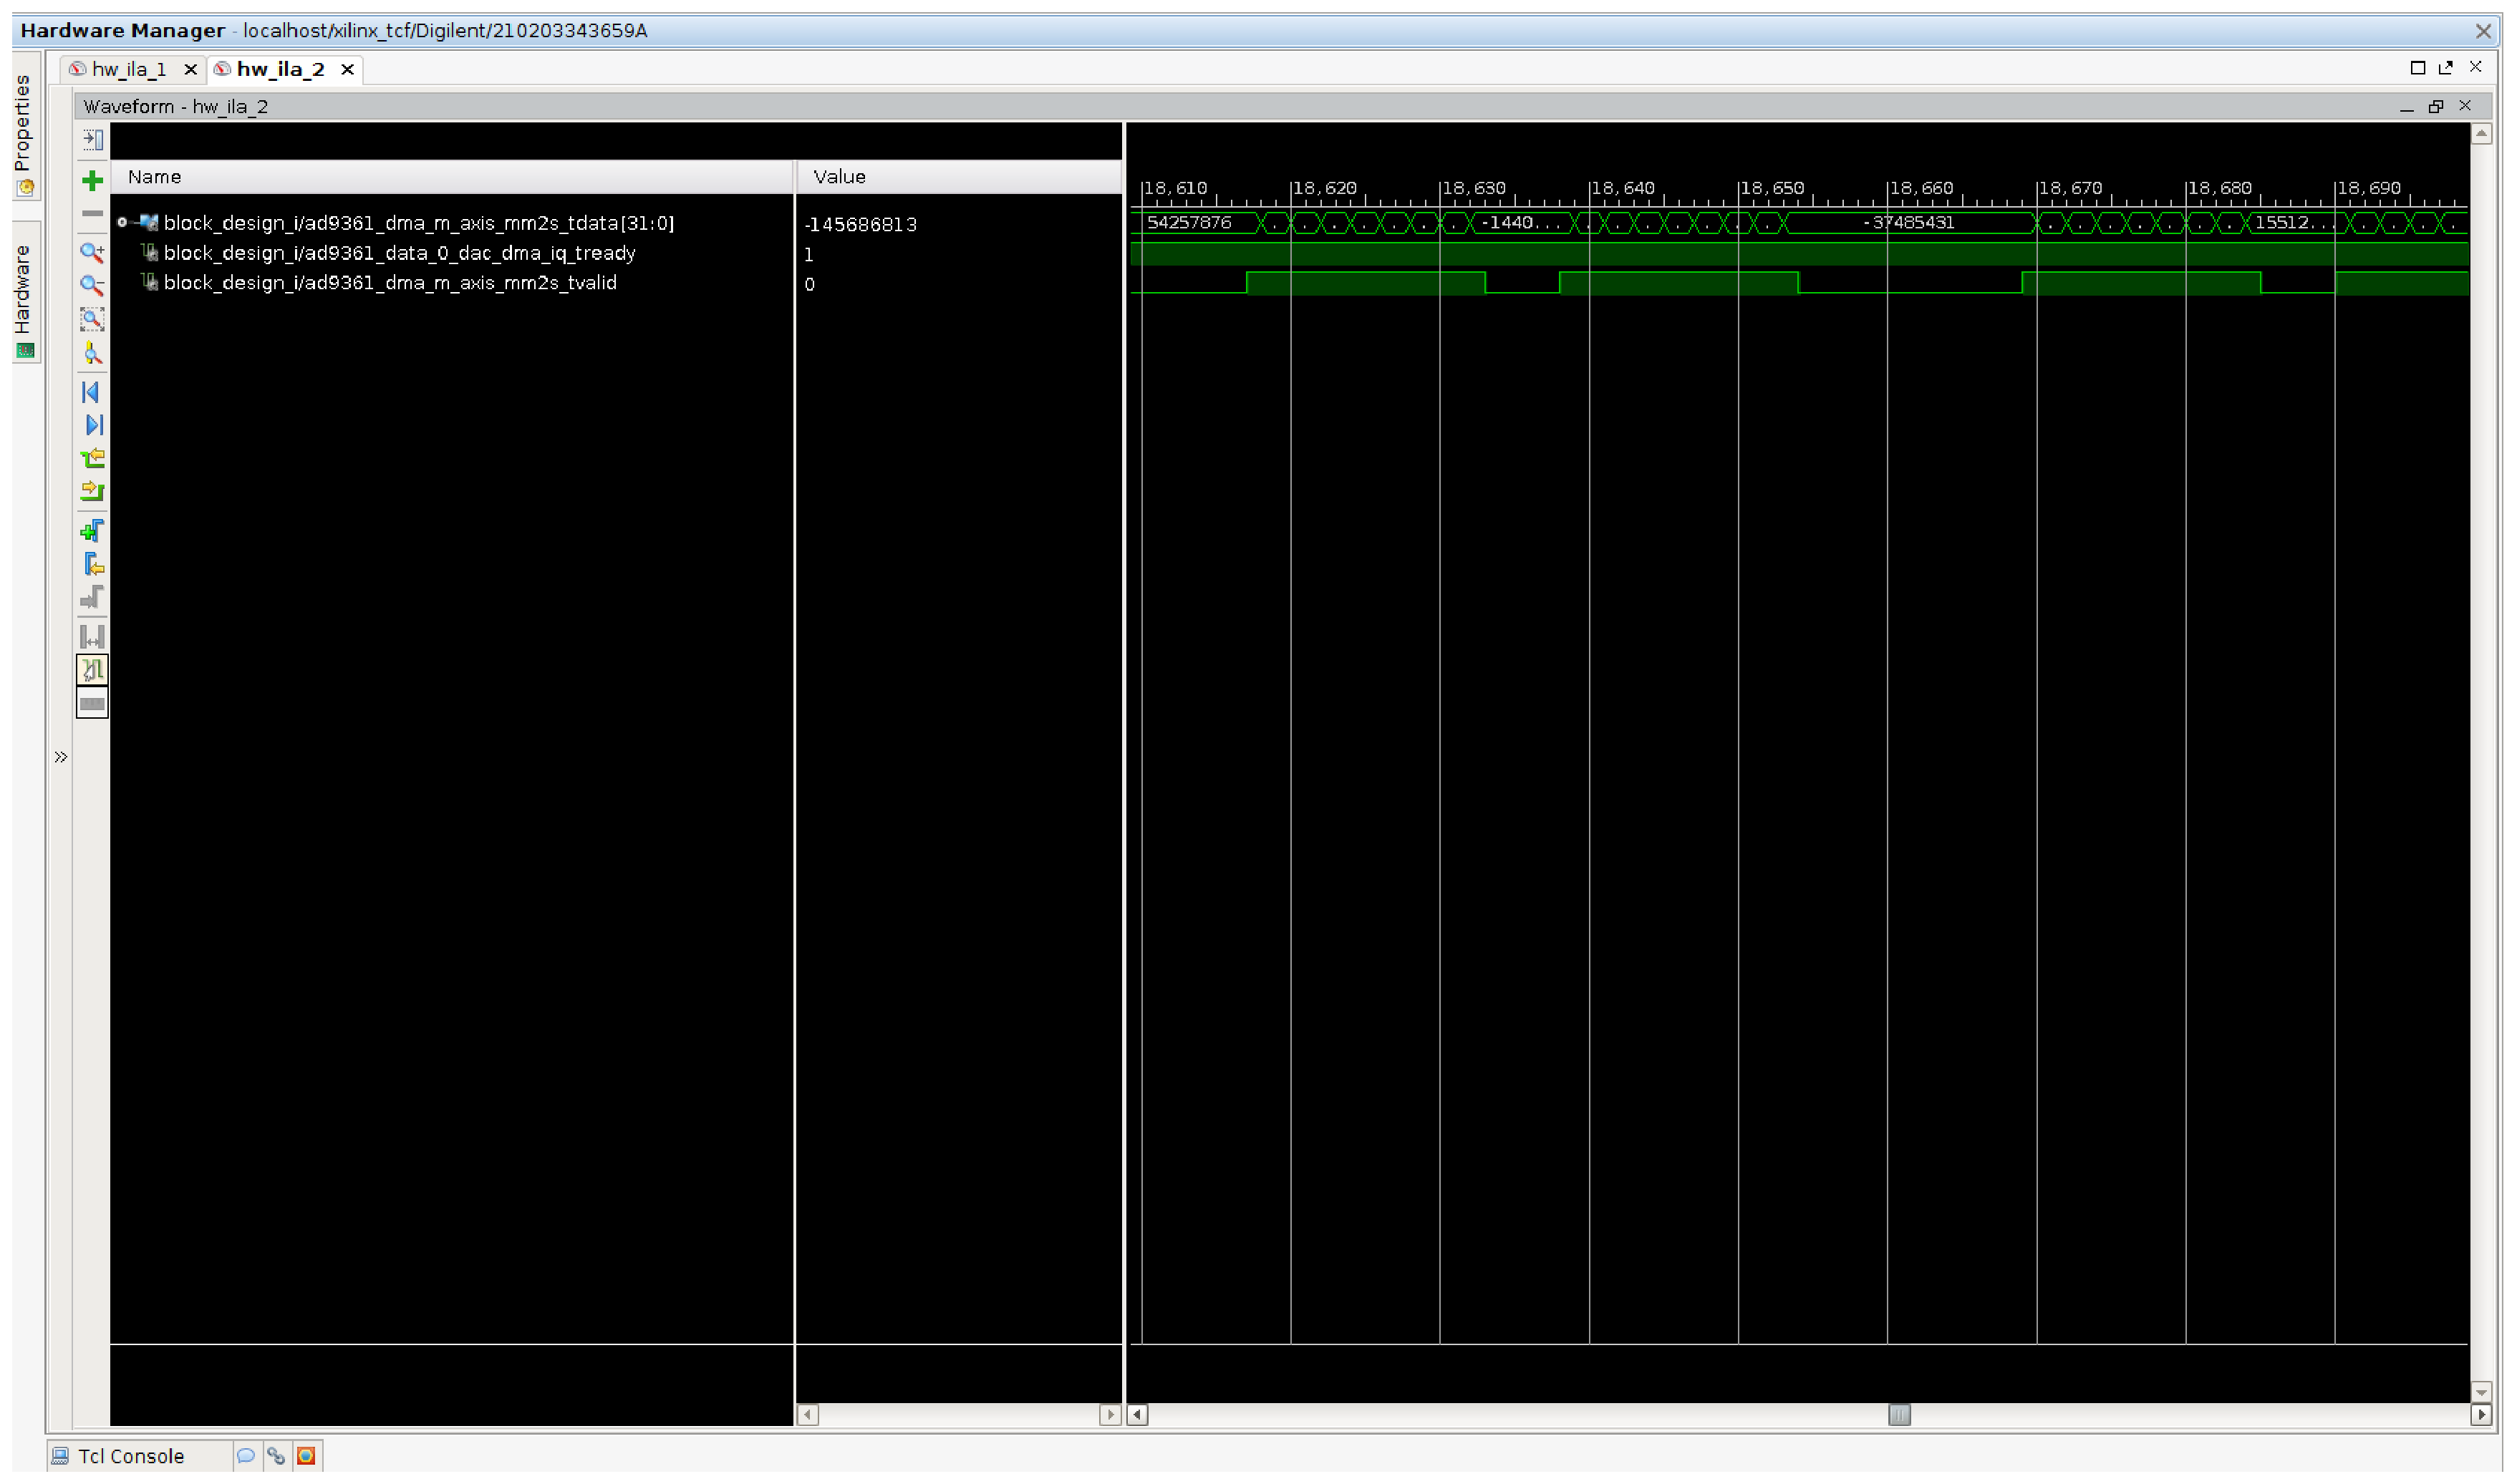
\includegraphics[width=0.85\textwidth]{./figures/ila_dataflow}
    \caption{ Digital Data read from memory by DMA.
    \label{fig:dataflowdig}}
\end{figure}

\begin{figure}[htbp]
    \centering
    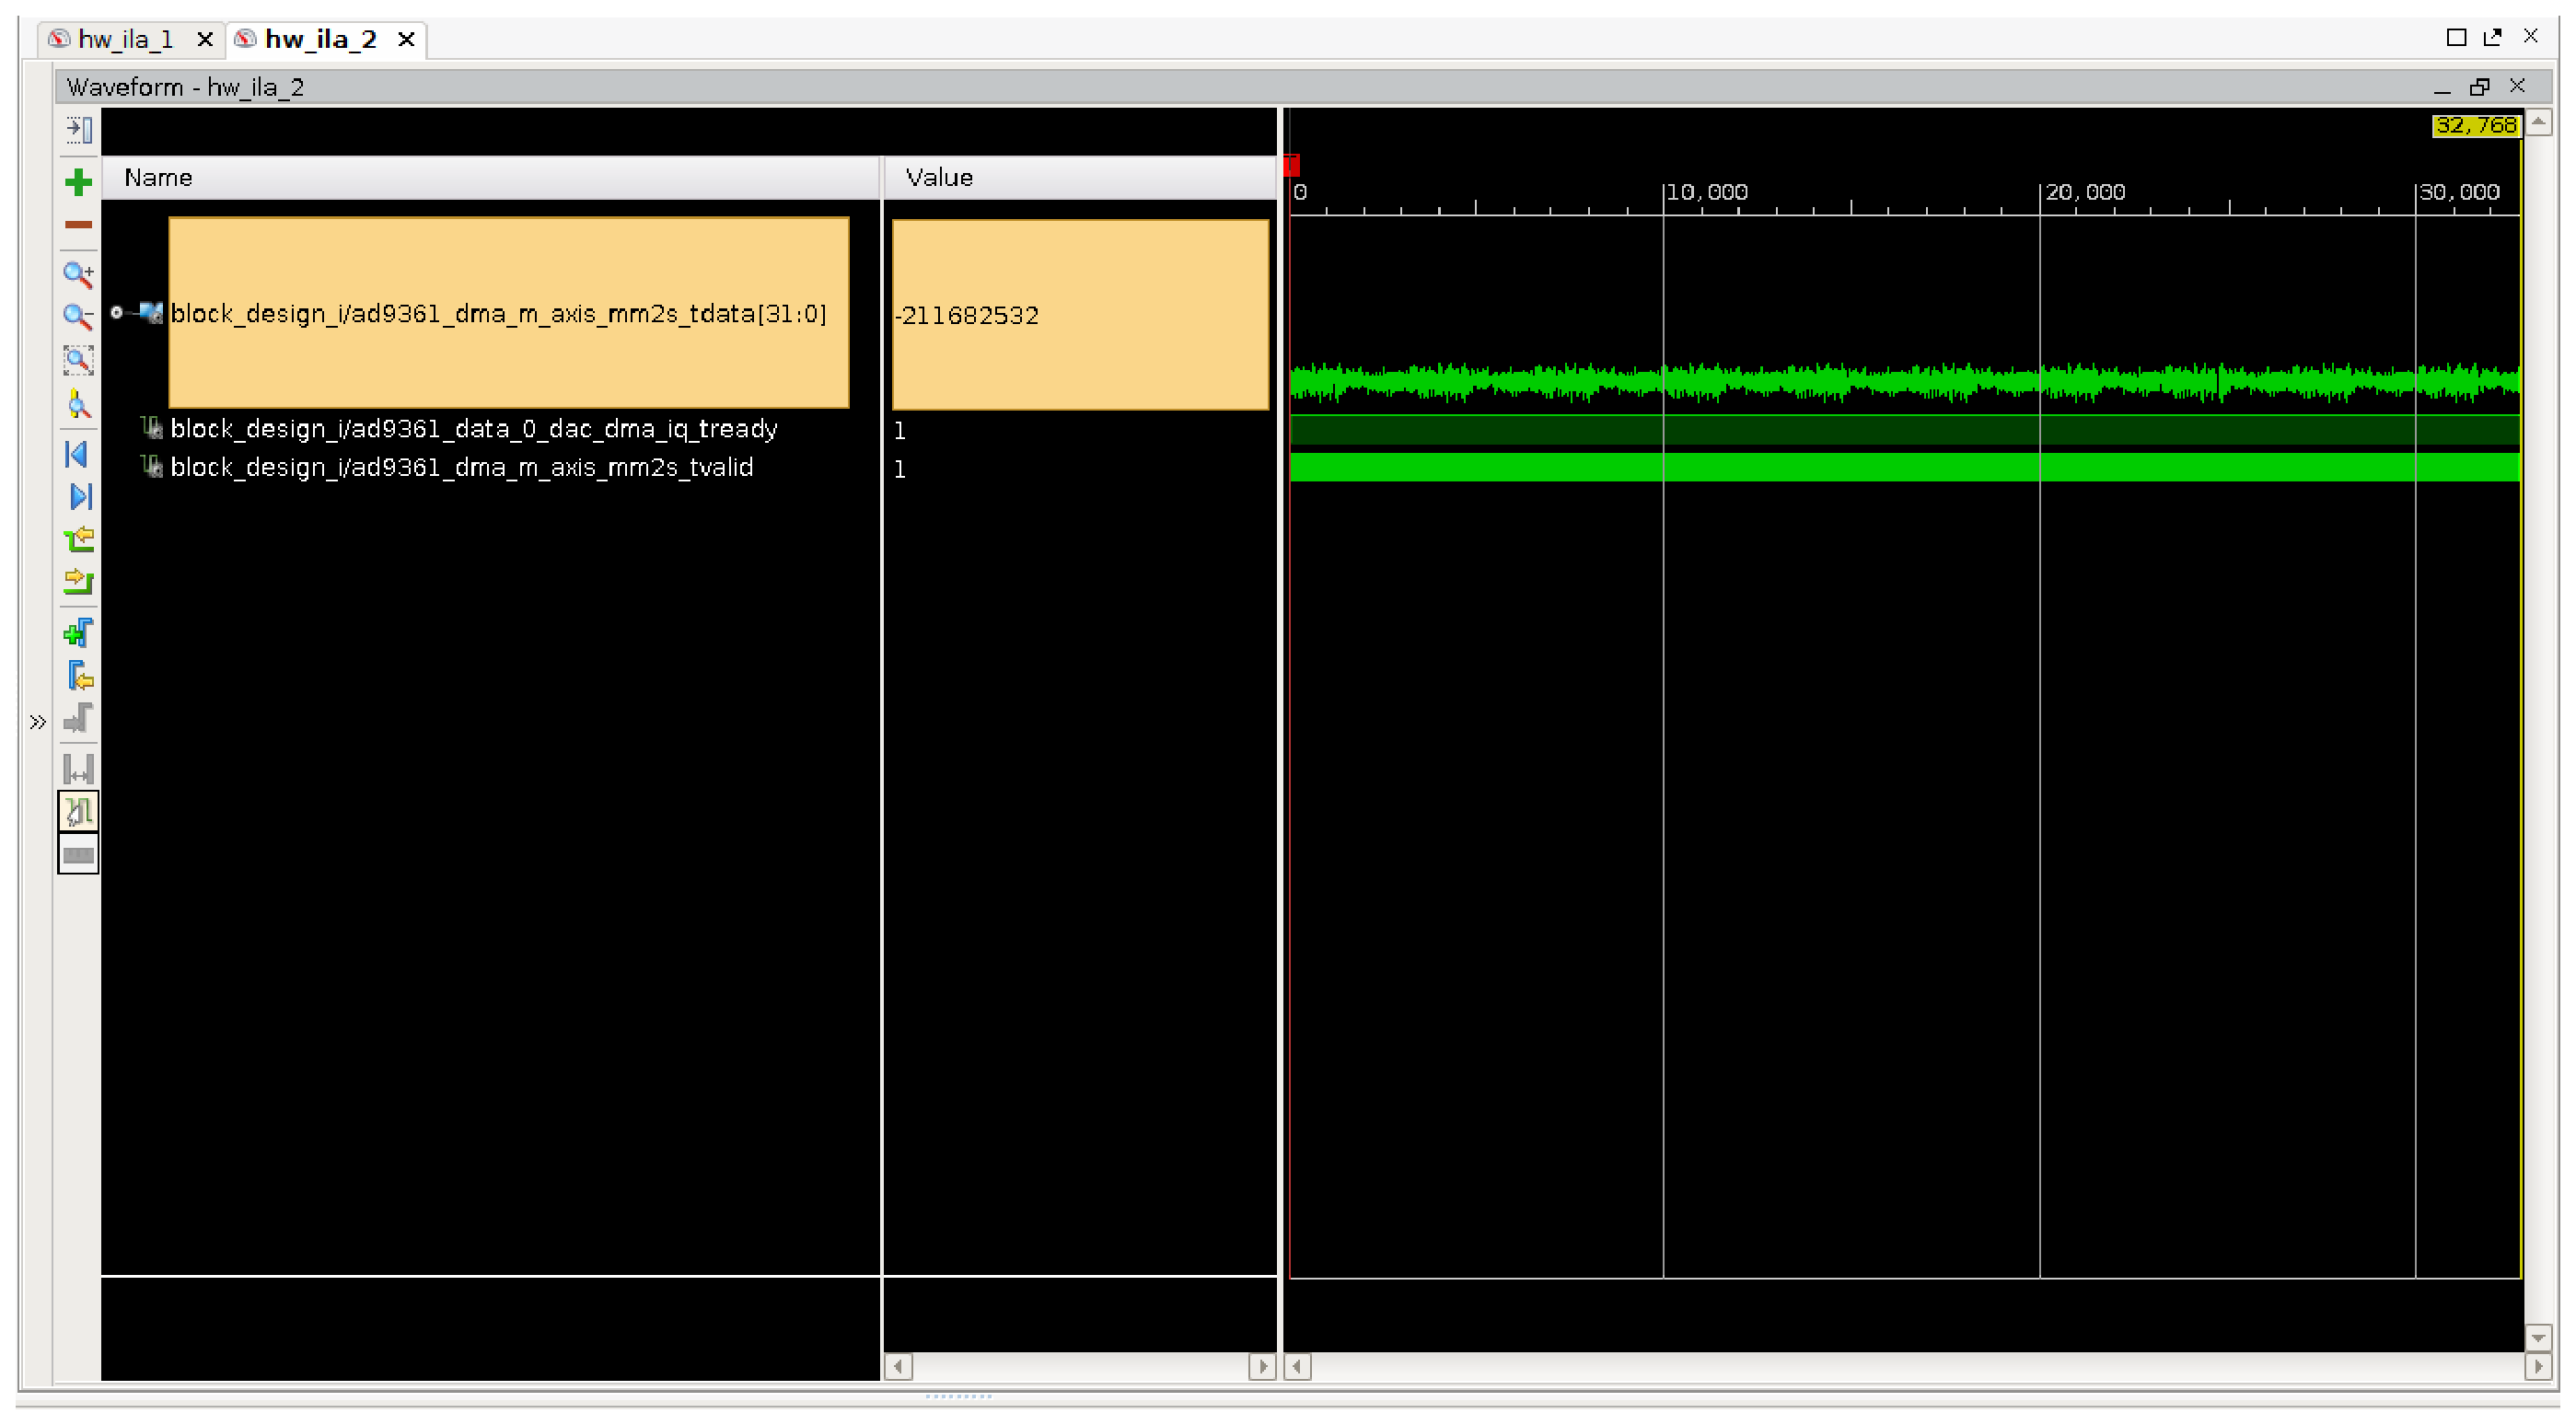
\includegraphics[width=0.85\textwidth]{./figures/ltedac_ila}
    \caption{ Analog form Data read form memory by DMA.
    \label{fig:dataflowana}}
\end{figure}

\begin{figure}[htbp]
    \centering
    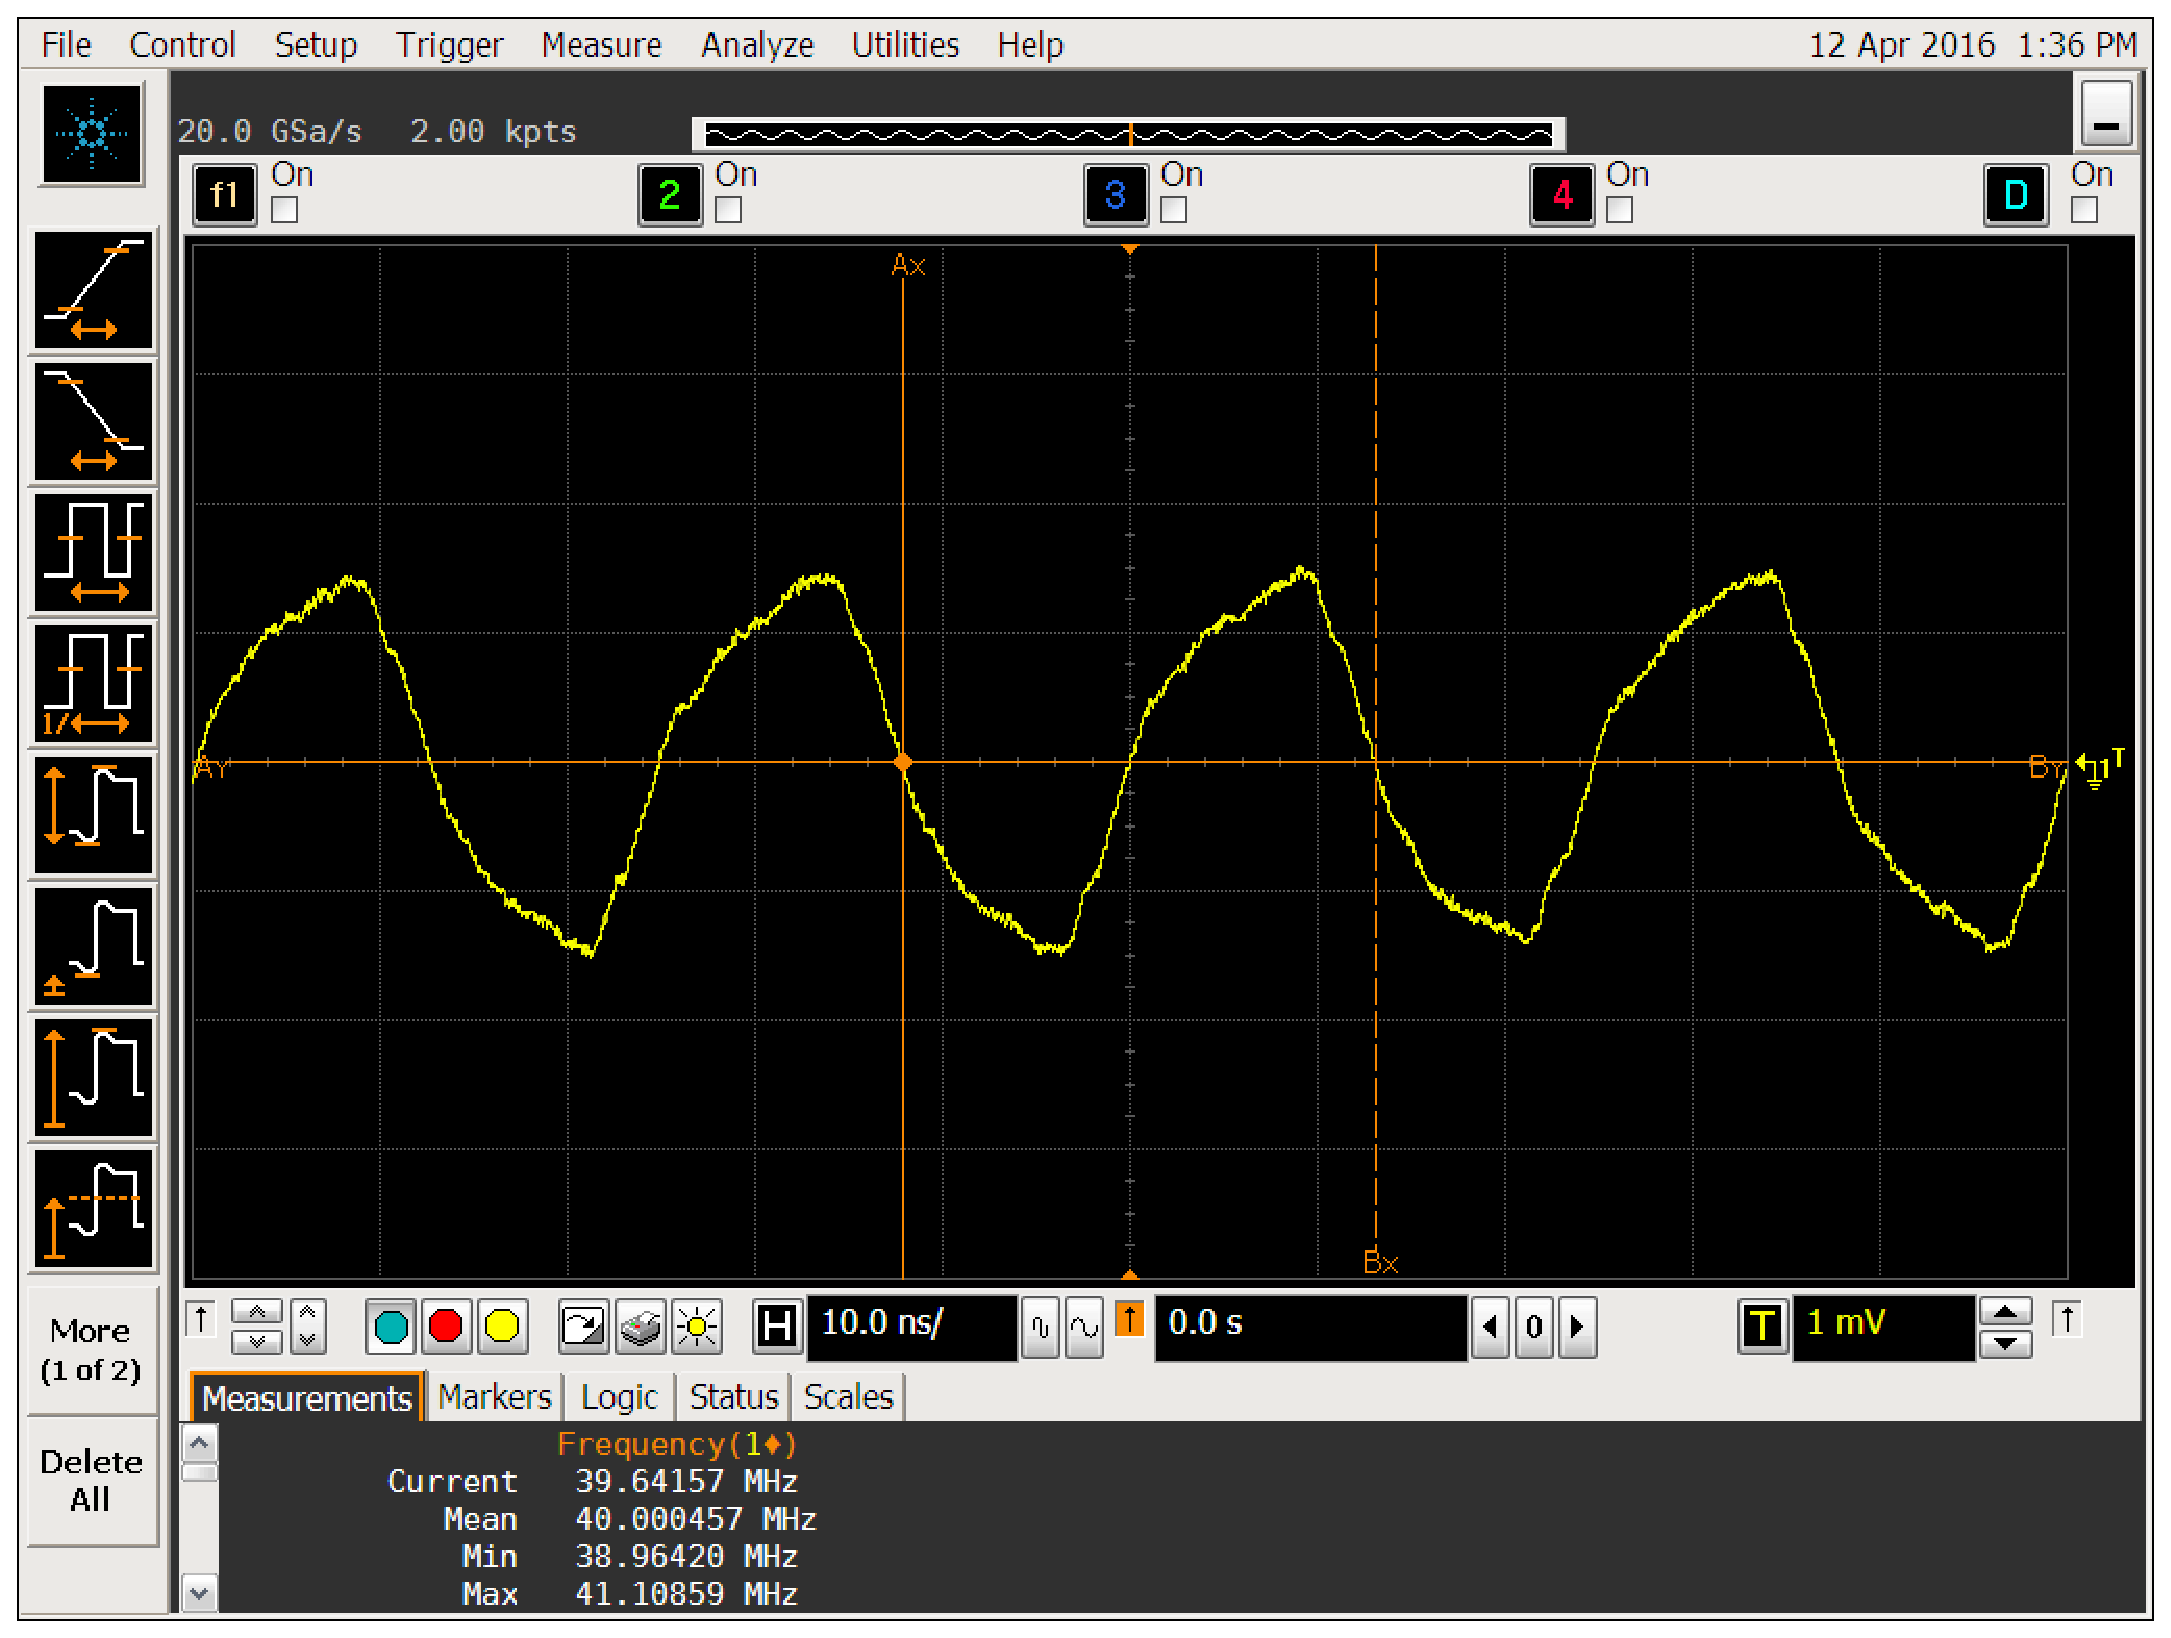
\includegraphics[width=0.85\textwidth]{./figures/oscill_ad9361_dac_clk}
    \caption{ DAC Clock Output
    \label{fig:dacclk}}
\end{figure}

\begin{figure}[htbp]
    \centering
    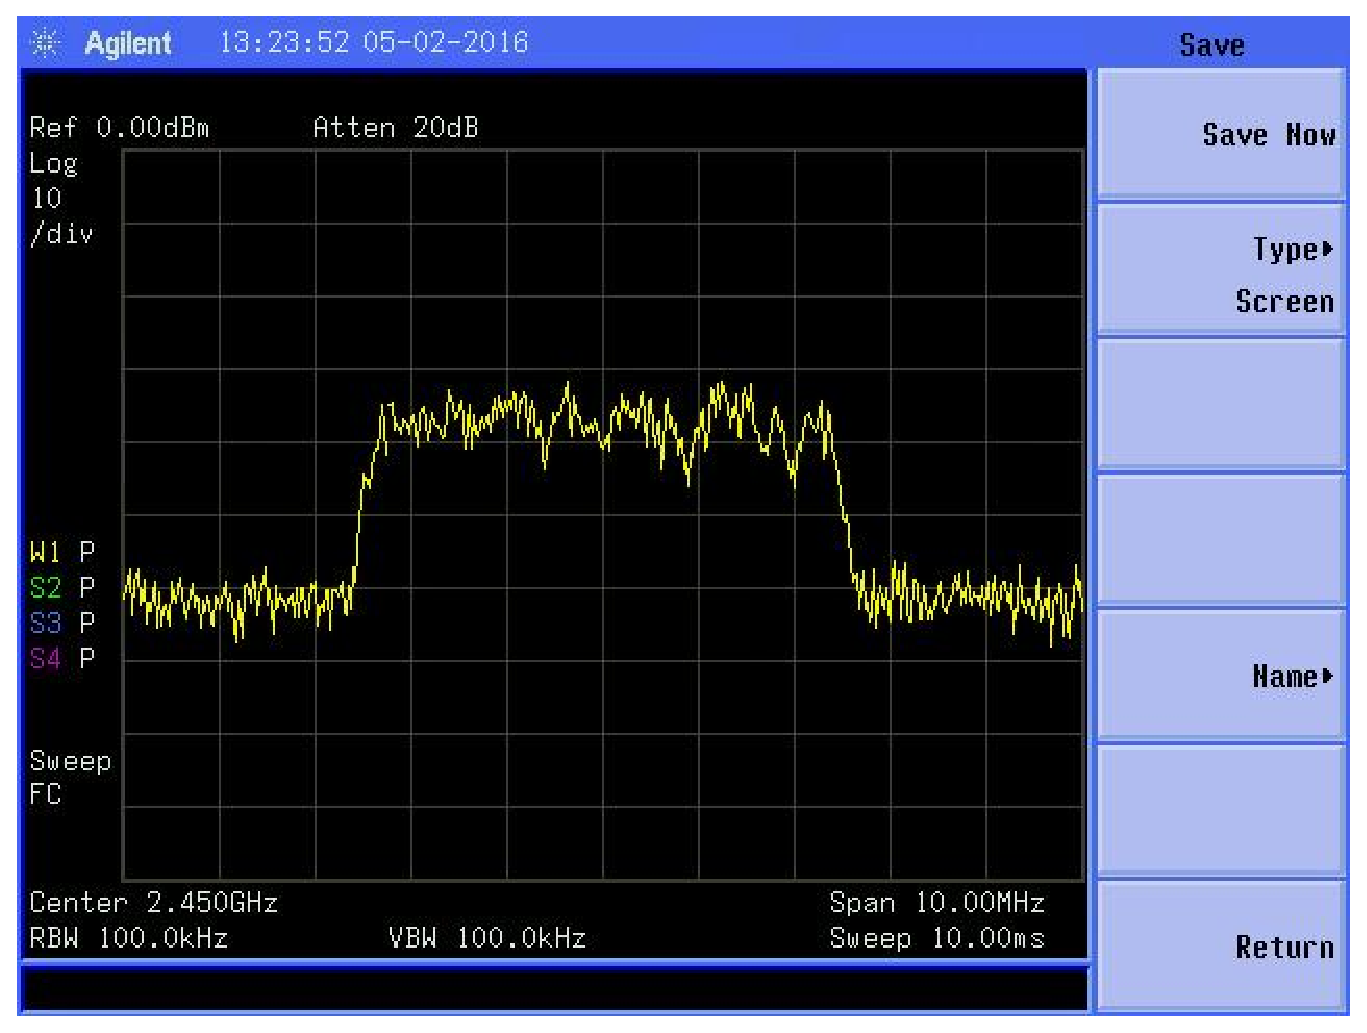
\includegraphics[width=0.85\textwidth]{./figures/lte_5m}
    \caption{ LTE signal output from FMComms2 Spectrum
    \label{fig:lte5m}}
\end{figure}

\vfill
\clearpage

\section{Reception Tests (ADC)}
\label{result:adc}

\begin{figure}[htbp]
    \centering
    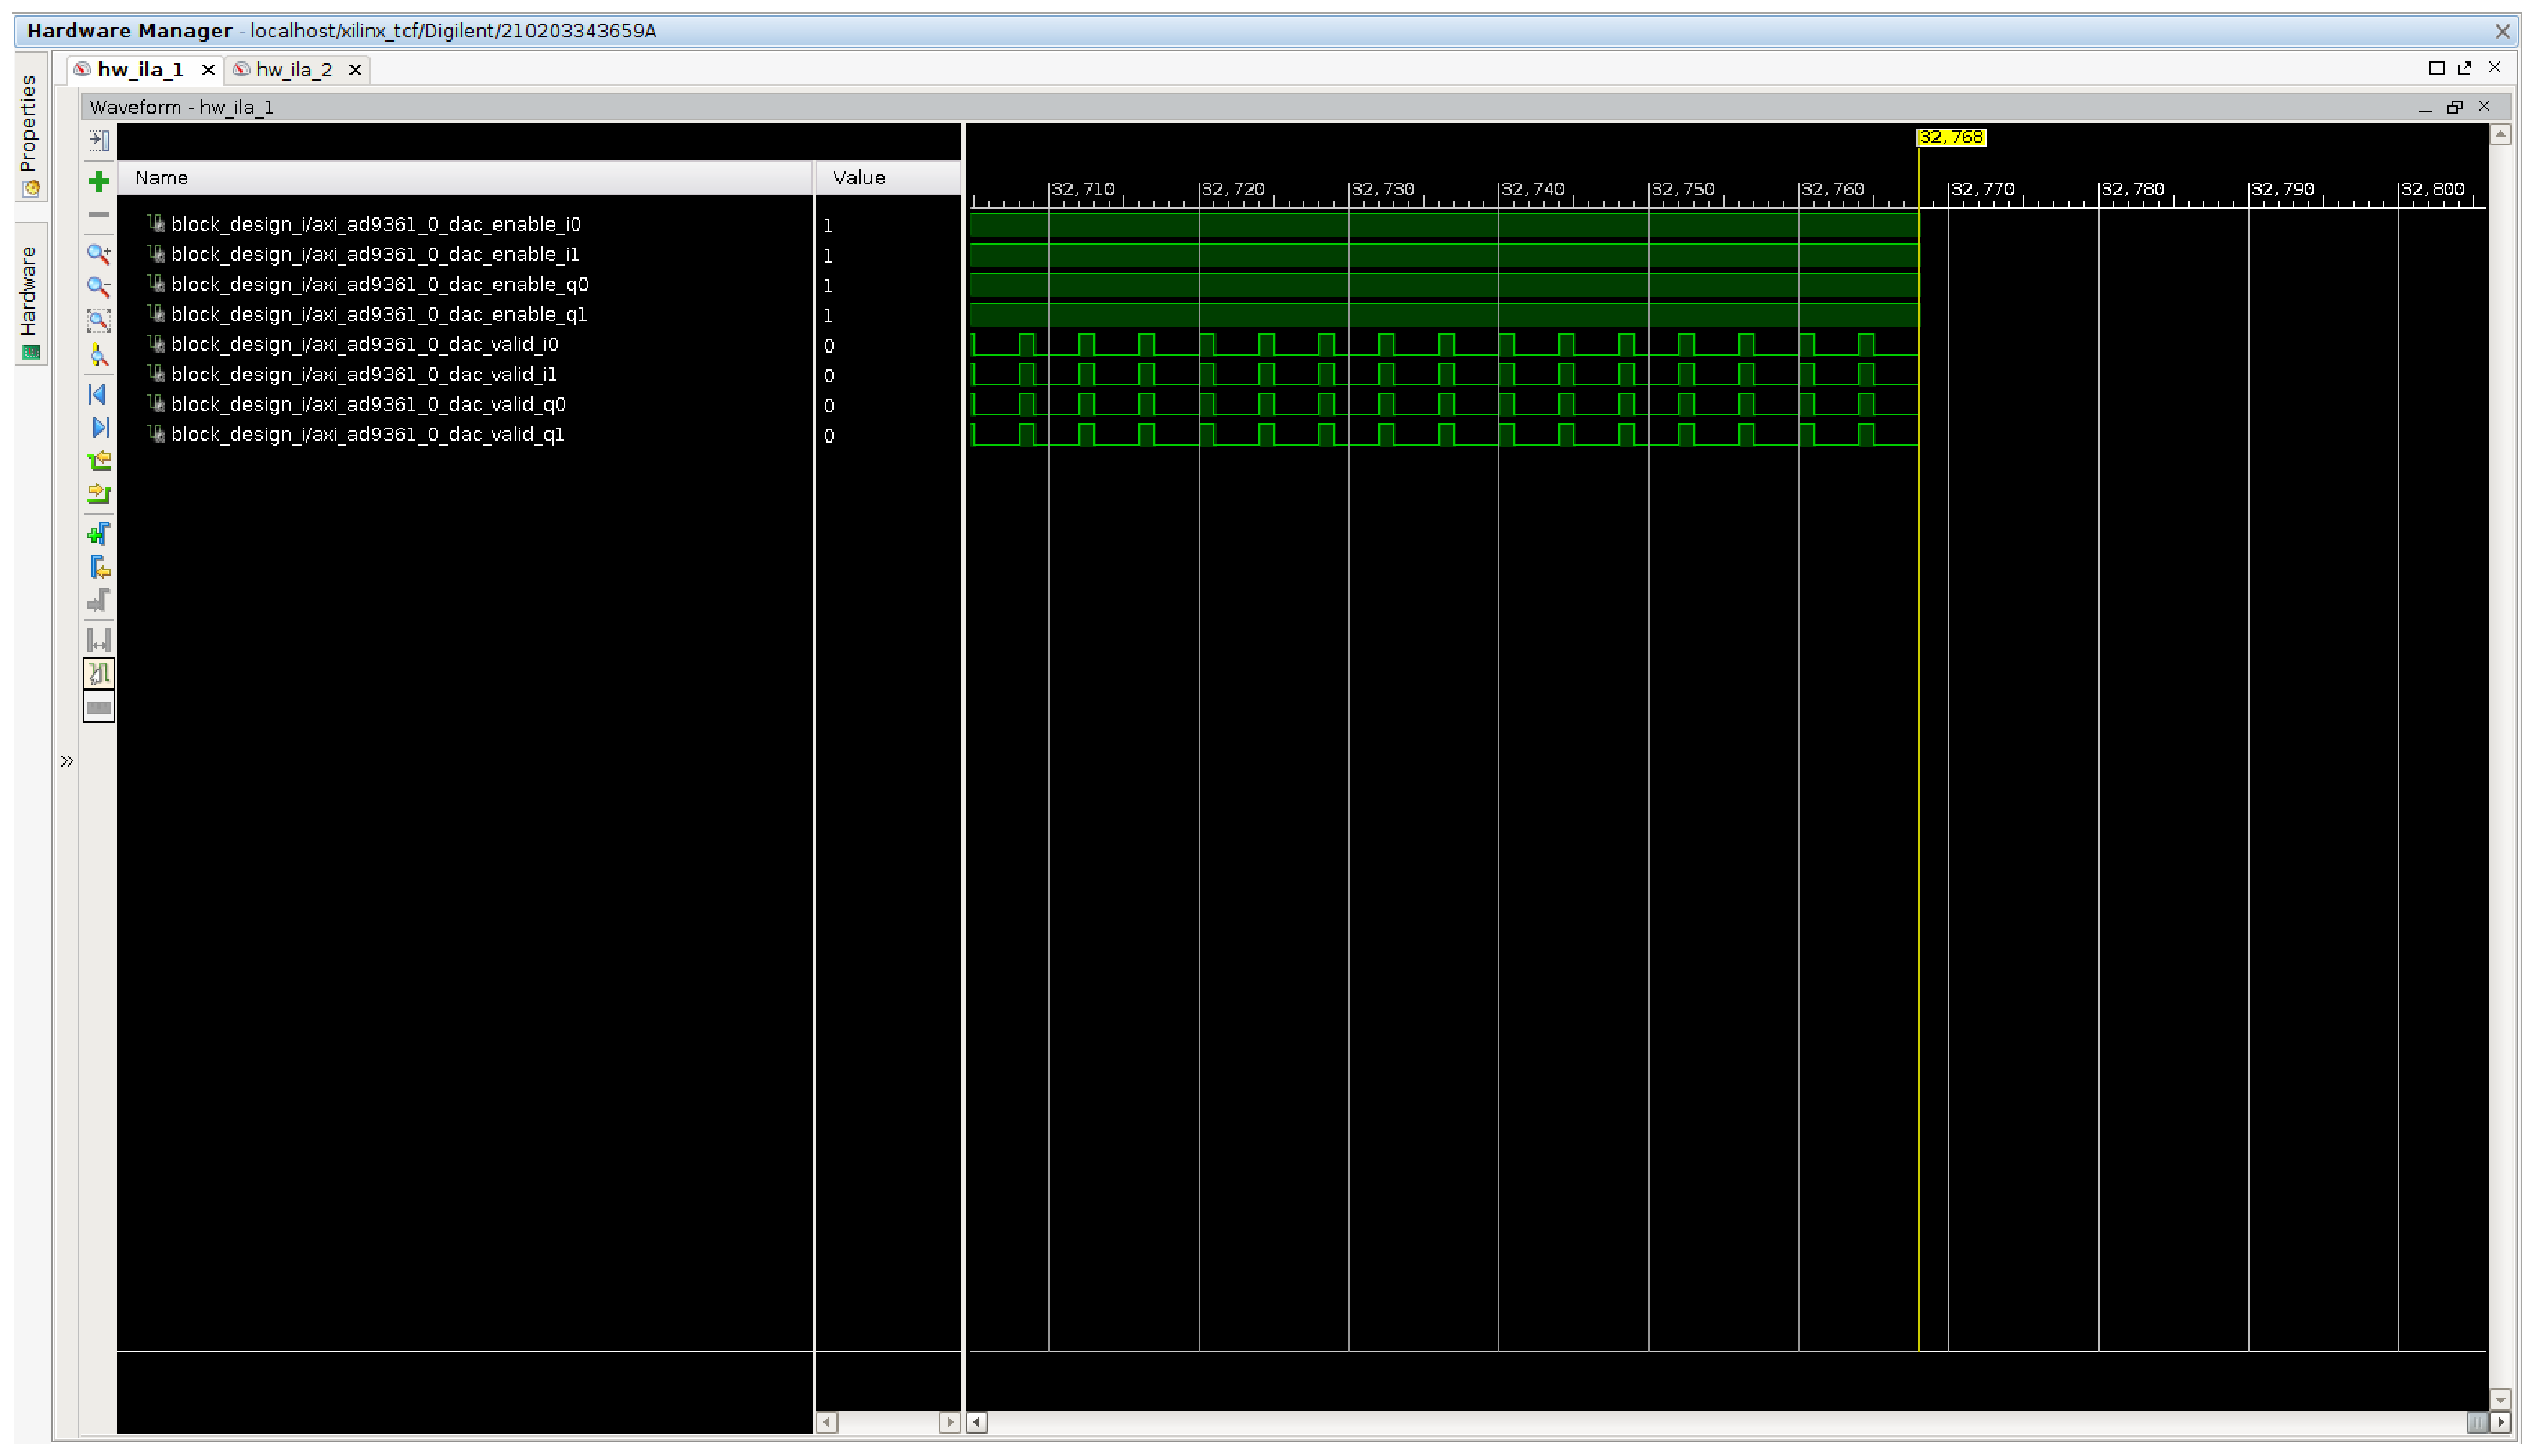
\includegraphics[width=0.85\textwidth]{./figures/dac_signals}
    \caption{ DAC signals controlling data writing
    \label{fig:adcsignals}}
\end{figure}

\vfill
\clearpage

\section{Optimum Results}
\label{result:optimum}

The expected transmission of lTE signals are below demonstrated by the Analog
Devices IIO scope application.

\begin{figure}[htbp]
    \centering
    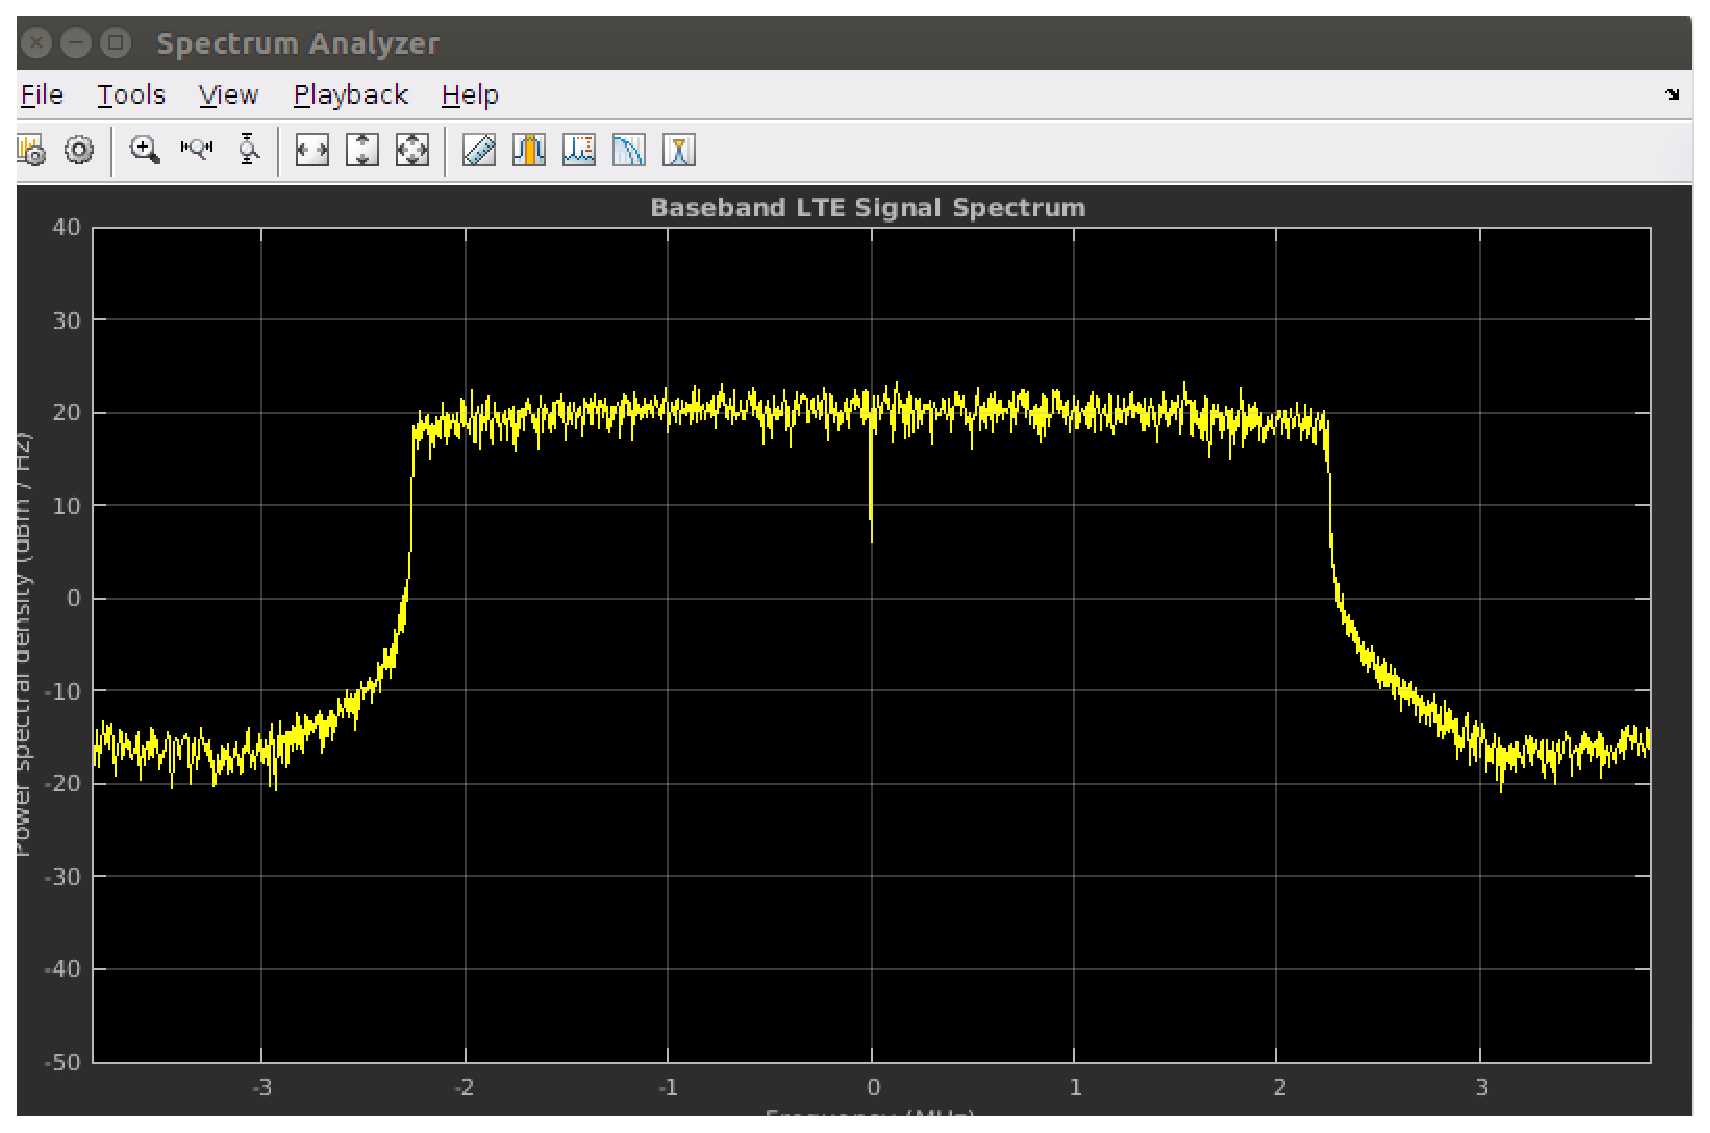
\includegraphics[width=0.65\textwidth]{./figures/lte_spectrum_iio}
    \caption{ LTE Spectrum
    \label{fig:ltespectrumiio}}
\end{figure}

\begin{figure}[htbp]
    \centering
    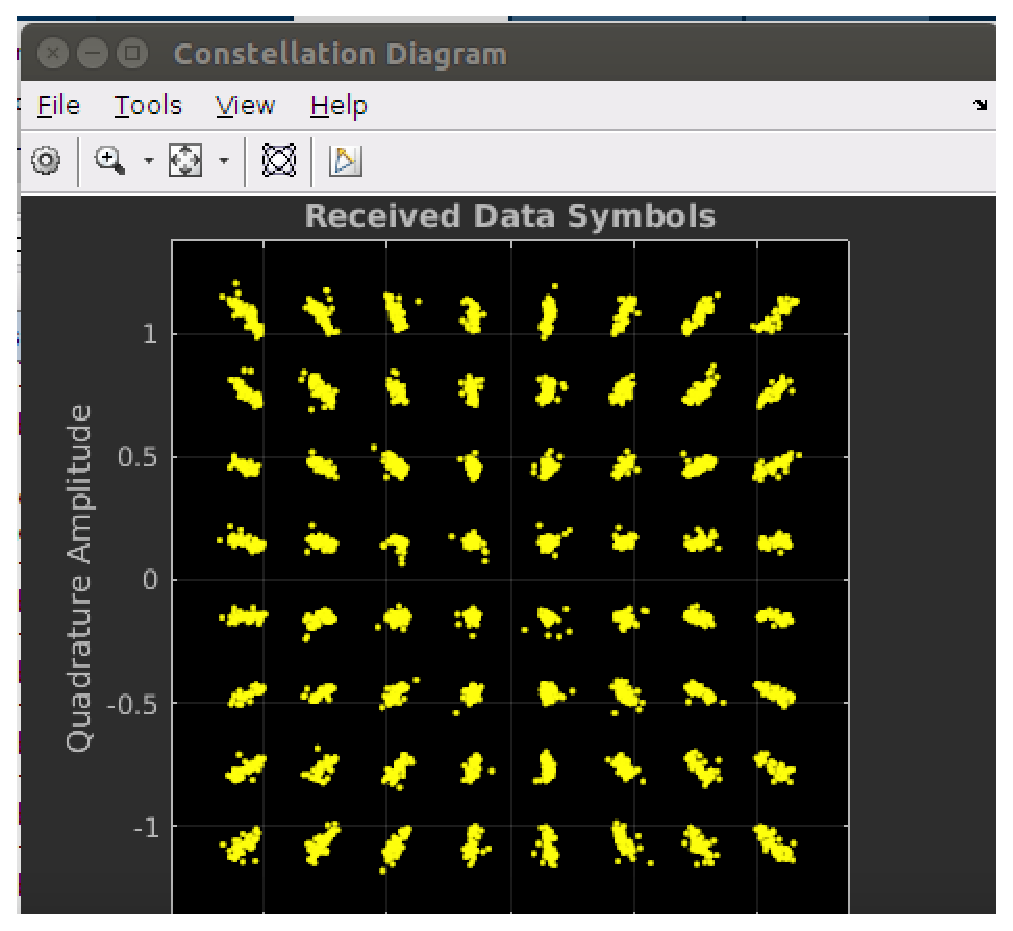
\includegraphics[width=0.65\textwidth]{./figures/lte_constellation_iio}
    \caption{ LTE Constellation
    \label{fig:lteconstellationiio}}
\end{figure}

\begin{figure}[htbp]
    \centering
    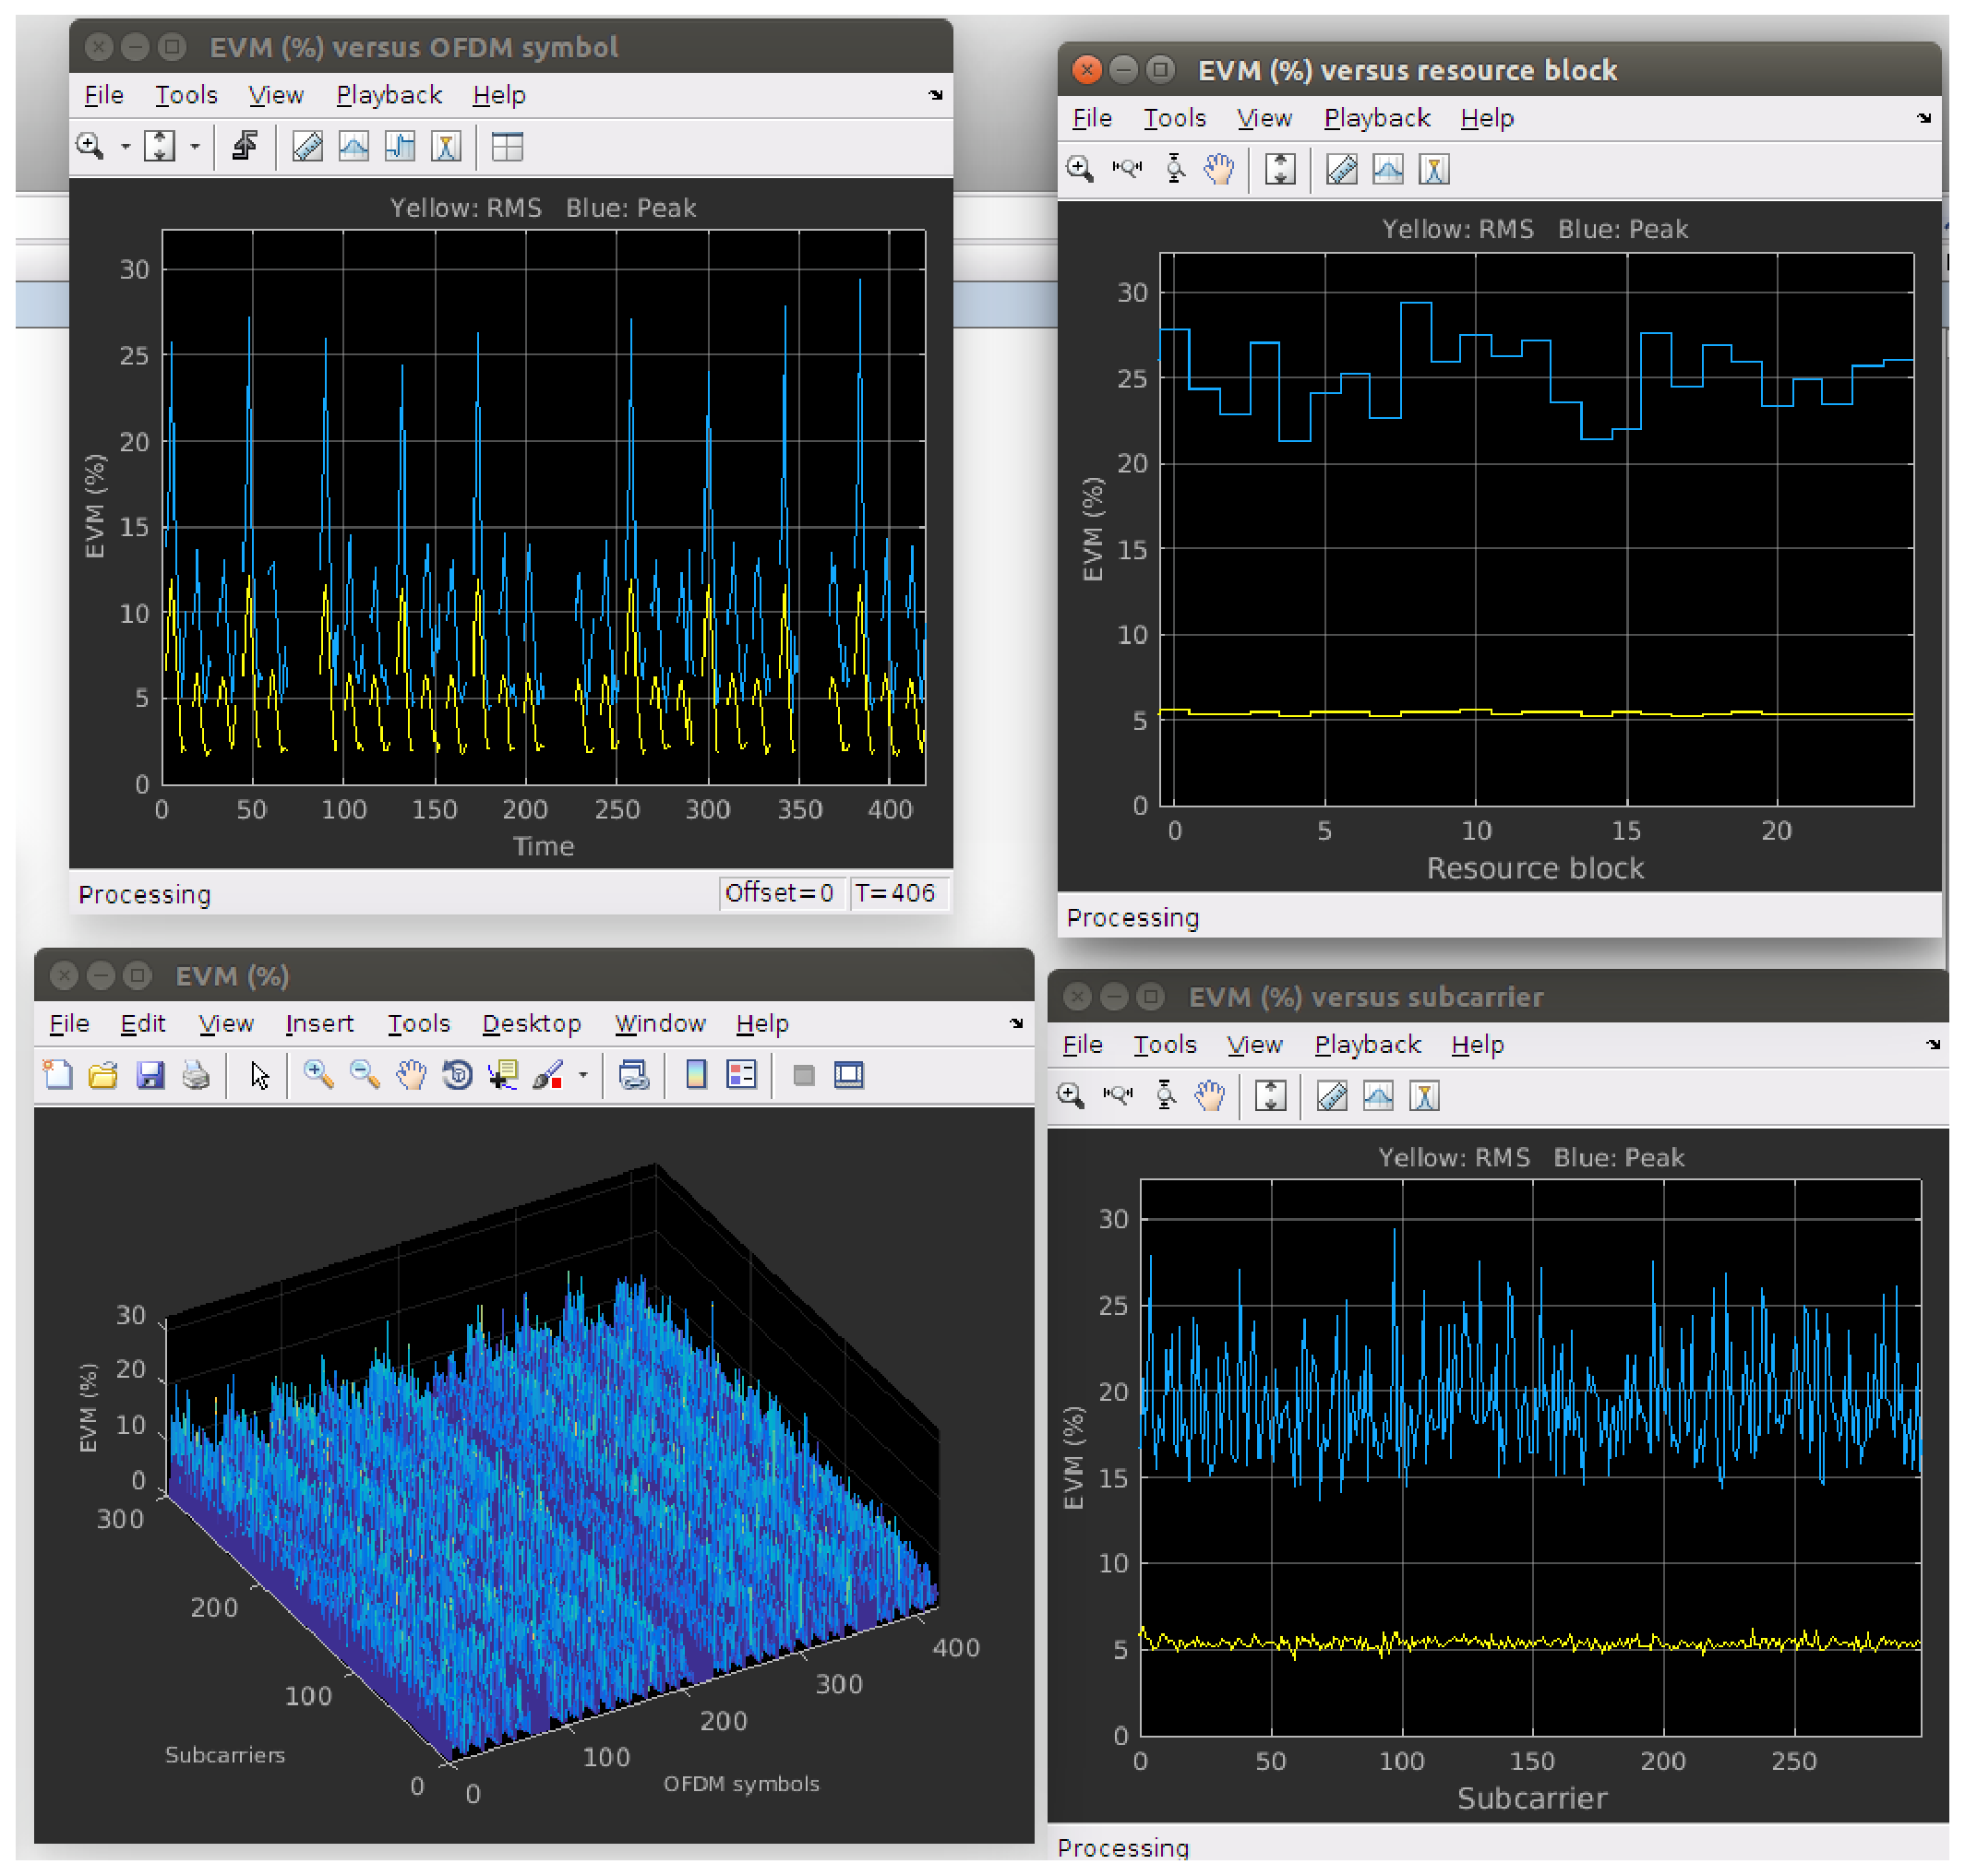
\includegraphics[width=0.85\textwidth]{./figures/lte_evm_iio}
    \caption{ LTE EVM
    \label{fig:lteevmiio}}
\end{figure}

\vfill
\clearpage

\part{Conclusion and Future Work}
\chapter{Conclusion}
\label{chap:conclusion}

\section{Conclusion}
\label{sec:conclusion}

The development of this setup was meant to be general and be used in both
research and academic environments. The process of implementing this setup went
through a myriad of fields in telecommunications and embedded systems, such as
communication protocols, embedded programming, electronics and many others,
being this setup a testbed for more complex processes inside the LTE band saves
a lot of time in development. \\

The FMComms2 board allows real-time and scalable change in parameters by
software or hardware signals, and it re-calibrates and reconfigures itself if
needed so, which makes a very good transceiver board to be used in a C-RAN
environment.\\

This setup was extensively documented and can be used in digital communication
classes to show how a real radio frontend system is made, of course there is
much to improve, there is no dynamic clock synchronization between the FPGA and
the FMComms2, there is no communication protocol between the FPGA (BBP) and the
external world other than the FMComms2 such things are necessary to have a real
frontend but were outside the scope of this project which was just to evaluate a
setup for a scalable and dynamically configurable frontend.\\

Although the FMComms2 and the FPGA operates on different clocks, thus no real
synchronization was implemented, this setup has the minimal capability of
transmitting and receiving signals and reconfigure itself on real-time, the main
goal of this work was reached, however there is much to explore with these tools
and devices.

\section{Future Works}
\label{sec:futurew}

Having finished this part of the work a natural sequel would be implementing
Ethernet connection driver in the FPGA, making it possible to receive data from
Ethernet and hand this to the transceiver board following the schematic on
figure \ref{fig:setupeth} idea. This would be a challenge because there is a lot
of things to consider, but the most problematic of them all is synchronization,
the clock in which everything inside the FPGA works is different from the AD9361
clock not only in frequency but in phase, this can bring a lot of problems,
however there is the possibility of feeding FMComms2 with an external clock
which would increase its performance.\\

With Ethernet it would be possible to generate the modulated samples and send
them trough air, just like Gnuradio + USRP and thus demodulate the received back
samples in the PC, however there is another possibility, modulation and
demodulation blocks implemented in the FPGA logic, thus much faster than the PC
ones and with partial reconfiguration there is the advantage of loading various
schemes of modulation/demodulation in the FPGA, implementing thus a very good
SDR. The Ethernet connection, is also very interesting for C-RAN
environment, because Ethernet is cheap and easy to implement.\\

\begin{figure}[htbp]
    \centering
    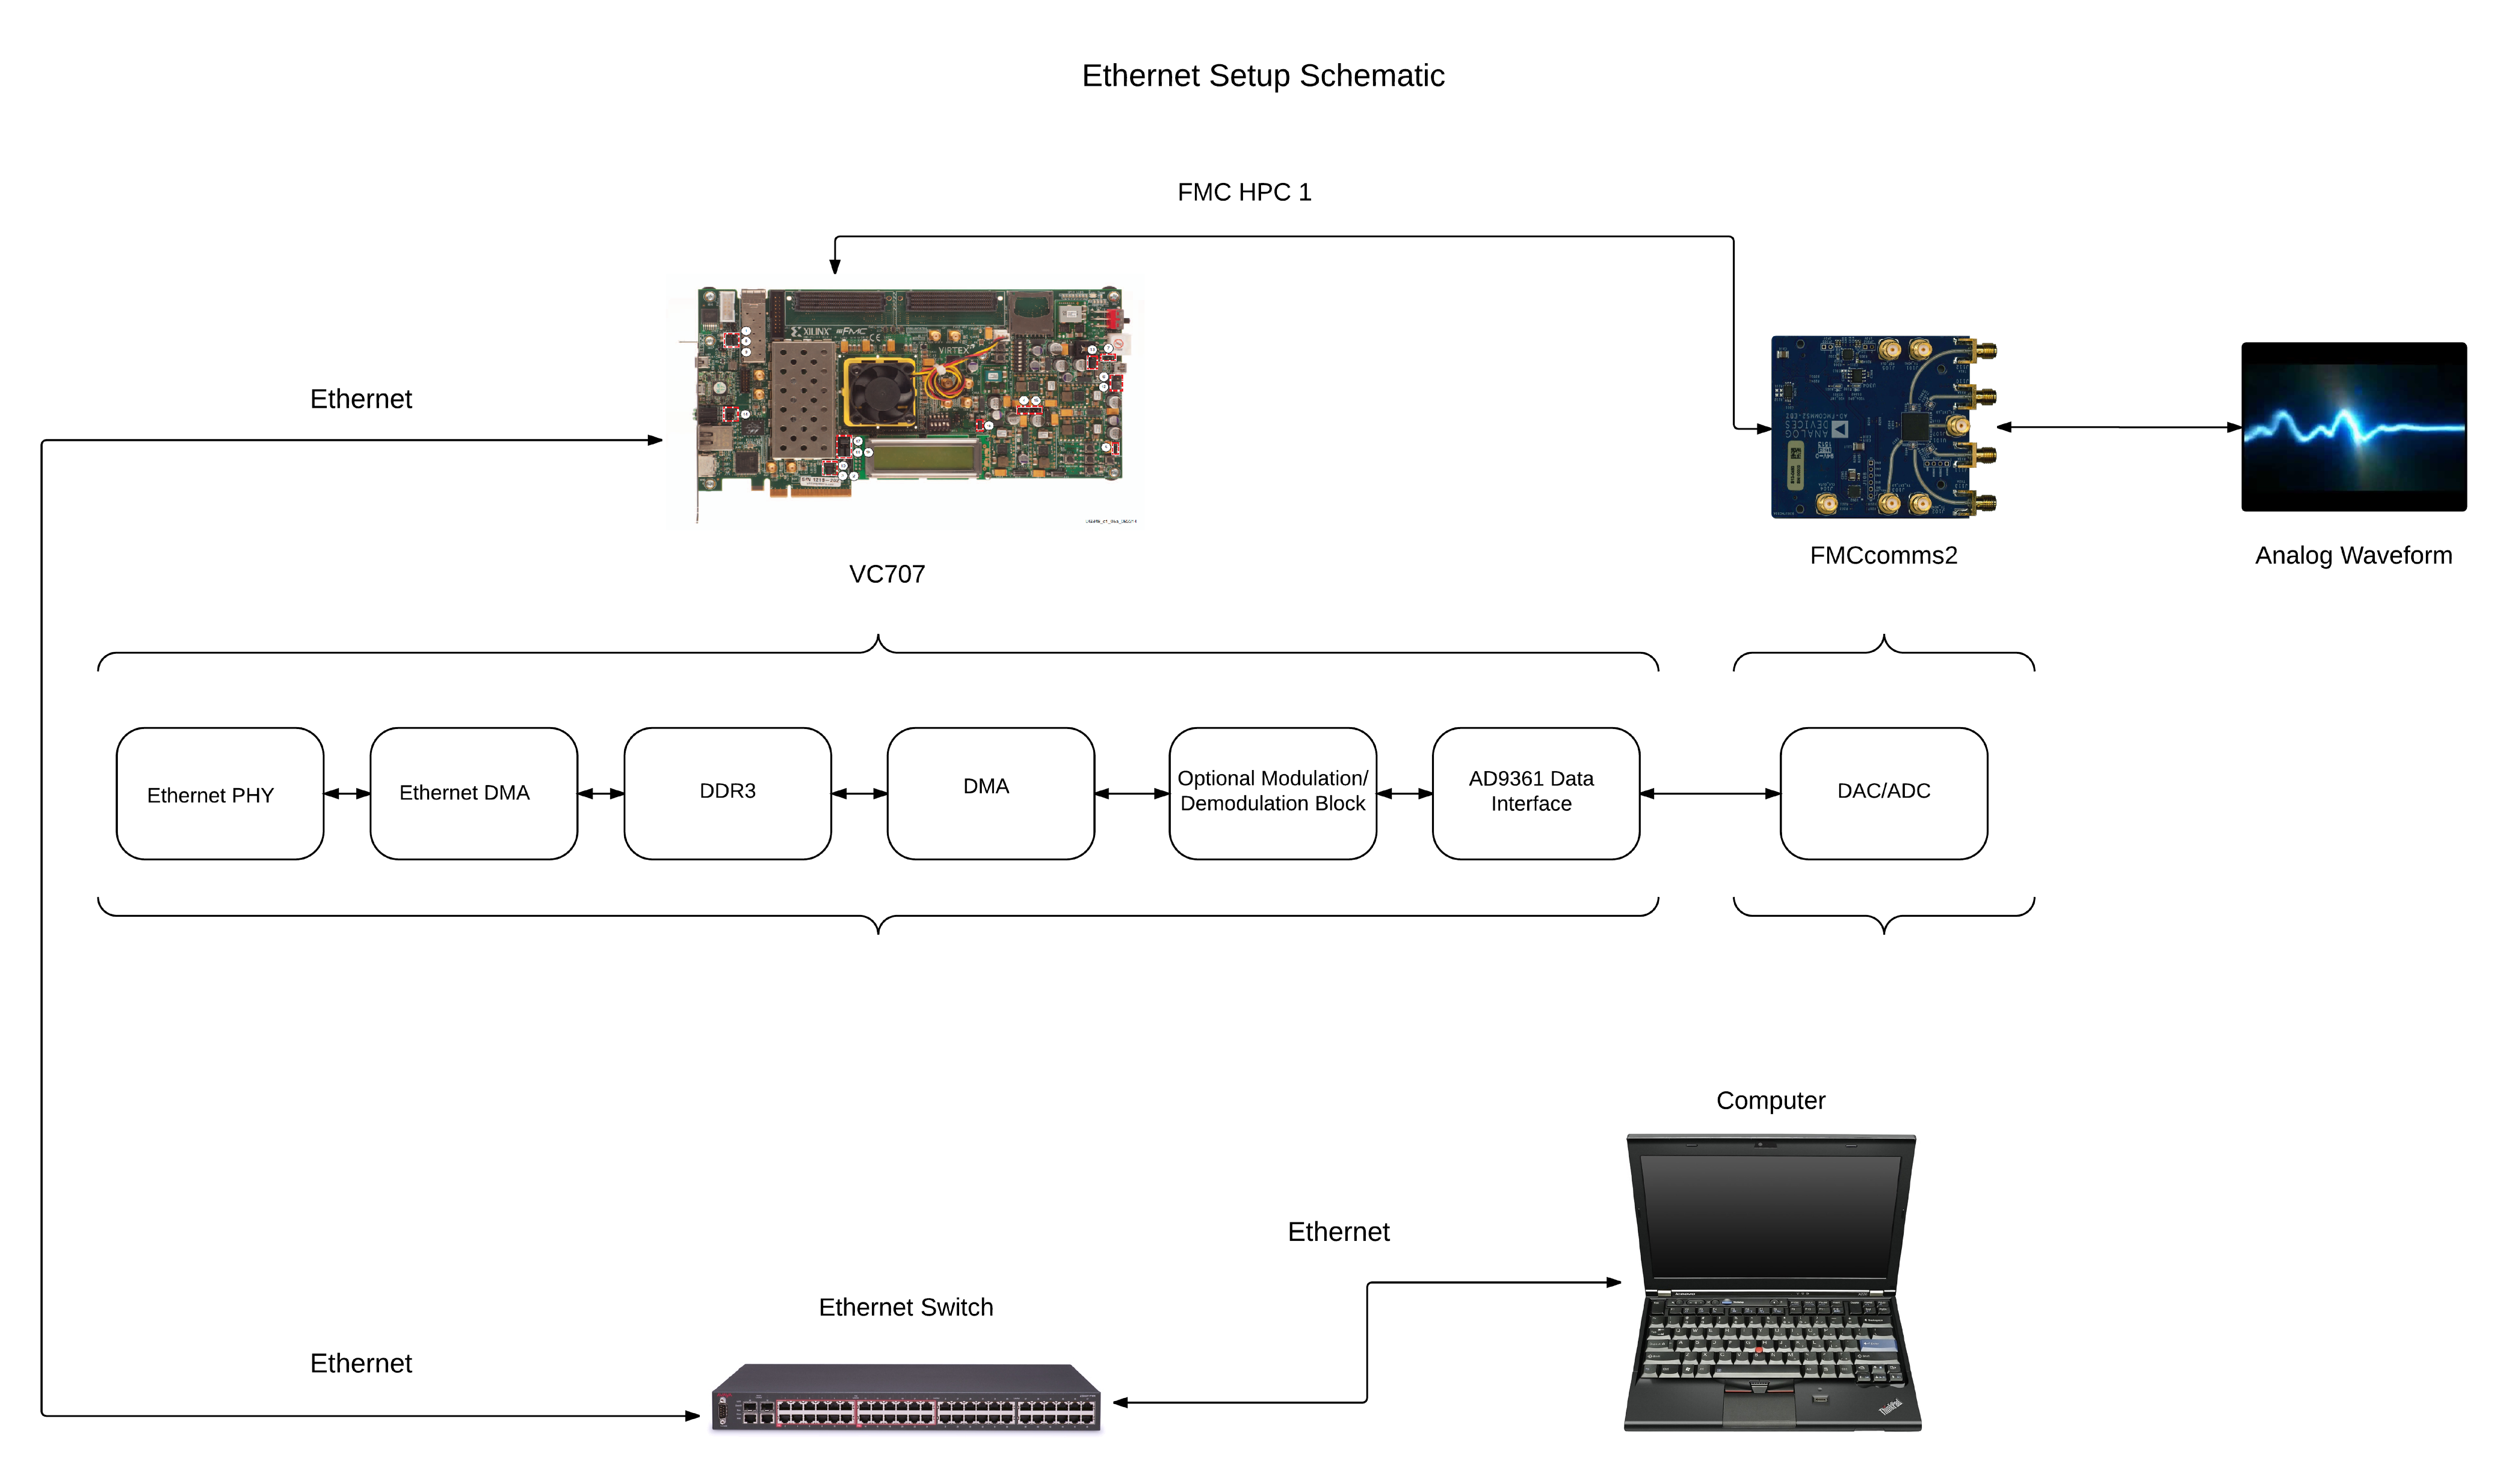
\includegraphics[width=0.95\textwidth]{./figures/eth_setup}
    \caption{ Setup Enhanced with Ethernet Connection
    \label{fig:setupeth}}
\end{figure}


%%%%%%%%%%%%%%%%%%%%%%%%%%%%%%%%%%`
%   Referencias bibliograficas   %
%%%%%%%%%%%%%%%%%%%%%%%%%%%%%%%%%%

\renewcommand\bibname{Refer�ncias Bibliogr�ficas}
%\bibliographystyle{../../../public/ABNT-20020112}
%\bibliographystyle{../public/IEEEtran}
%\bibliographystyle{../../../Public/IEEEtran_pt}
\bibliographystyle{abnt}
\bibliography{references}

%temorary tag just while there is no \citation
%eliminates no \citation error
\nocite{*}

\clearpage

%%%%%%%%%%%%%%%%%%%%%
%   Apêndices    %
%%%%%%%%%%%%%%%%%%%%%

\appendix
\input{appendix/append_pll}
\input{appendix/append_fpga_flow}
\chapter{AD9361 NO-OS Driver}
\label{app:noos}


\begin{table}[]
\centering
\caption{ad9361 Base Configuration}
\label{tab:basecf}
\begin{tabular}{|l|l|l|}
\hline
\textbf{Linux Device Tree Attribute}               & \textbf{No-OS AD9361\_ParamInit structure member}  & \textbf{Description}                              \\ \hline
adi,2rx-2tx-mode-enable                   & two\_rx\_two\_tx\_mode\_enable            & Use 2Rx2Tx mode - default 1Rx1Tx (AD9364 must clear this)           \\ \hline
adi,frequency-division-duplex-mode-enable & frequency\_division\_duplex\_mode\_enable & Use FDD mode - default TDD                                          \\ \hline
adi,tdd-use-dual-synth-mode-enable        & tdd\_use\_dual\_synth\_mode\_enable       & In TDD mode use Dual Synth mode - default only one Synth is enabled \\ \hline
adi,tdd-use-fdd-vco-tables-enable         & tdd\_use\_fdd\_vco\_tables\_enable        & In TDD mode use the FDD VCO tables                                  \\ \hline
adi,tdd-skip-vco-cal-enable               & tdd\_skip\_vco\_cal\_enable               & Option to skip VCO cal in TDD mode when moving from TX/RX to Alert  \\ \hline
\end{tabular}
\end{table}

\begin{table}[]
\centering
\caption{ENSM Control}
\label{tab:ensm}
\begin{tabular}{|l|l|l|}
\hline
\textbf{Linux Device Tree Attribute}                  & \textbf{No-OS AD9361\_ParamInit structure member}      & \textbf{Description}                                                                \\ \hline
adi,ensm-enable-pin-pulse-mode-enable                 & ensm\_enable\_pin\_pulse\_mode\_enable                 & ENSM control Pins (ENABLE/TXNRX) use Pulse mode - default Level Mode                \\ \hline
adi,ensm-enable-txnrx-control-enable                  & ensm\_enable\_txnrx\_control\_enable                   & ENSM control Pins (ENABLE/TXNRX) control ENSM state - default SPI writes            \\ \hline
adi,frequency-division-duplex-independent-mode-enable & frequency\_division\_duplex\_independent\_mode\_enable & Use independent FDD mode - allows individual control over RX and TX (Pin Mode Only) \\ \hline
\end{tabular}
\end{table}

\begin{table}[]
\centering
\begin{adjustbox}{width=1\textwidth}
\label{my-label}
\begin{tabular}{|l|l|l|}
\hline
\textbf{Linux Device Tree Attribute}         & \textbf{No-OS AD9361\_ParamInit structure member} & \textbf{Description}                                                                   \\ \hline
adi,rx-synthesizer-frequency-hz              & rx\_synthesizer\_frequency\_hz                    & RX LO power-up Frequency in Hz                                                         \\ \hline
adi,tx-synthesizer-frequency-hz              & tx\_synthesizer\_frequency\_hz                    & TX LO power-up Frequency in Hz                                                         \\ \hline
adi,tx-fastlock-delay-ns                     & tx\_fastlock\_delay\_ns                           & TX fastlock delay in ns                                                                \\ \hline
adi,rx-fastlock-delay-ns                     & rx\_fastlock\_delay\_ns                           & RX fastlock delay in ns                                                                \\ \hline
adi,rx-fastlock-pincontrol-enable            & rx\_fastlock\_pincontrol\_enable                  & RX fastlock pin control enable                                                         \\ \hline
adi,tx-fastlock-pincontrol-enable            & tx\_fastlock\_pincontrol\_enable                  & RX fastlock pin control enable                                                         \\ \hline
adi,trx-synthesizer-target-fref-overwrite-hz & trx\_synthesizer\_target\_fref\_overwrite\_hz     & This allows forcing a lower F\_REF window (worse phase noise, better fractional spurs) \\ \hline
adi,external-tx-lo-enable                    & external\_tx\_lo\_enable                          & Enables external LO for TX                                                             \\ \hline
adi,external-rx-lo-enable                    & external\_rx\_lo\_enable                          & Enables external LO for RX                                                             \\ \hline
\end{tabular}
\end{adjustbox}
\caption{lol}
\end{table}


%%%%%%%%%%%%%%%%%%%%%
%   Página em branco    %
%%%%%%%%%%%%%%%%%%%%%

\newpage
\thispagestyle{empty}
\mbox{}

%% -- Termino do TCC
\end{document}
